% REMEMBER: You must not plagiarise anything in your report. Be extremely careful.

\documentclass{l4proj}

    
%
% put any additional packages here
%

\begin{document}

%==============================================================================
%% METADATA
\title{Privacy Preservation in Human Motion Analysis}
\author{Boondirek Kanjanapongporn}
\date{January 14, 2024}

\maketitle

%==============================================================================
%% ABSTRACT
\begin{abstract}
    
Integrating deep learning techniques into human motion analysis, particularly within the healthcare sector, has shown significant promise for detecting issues based on patient movement. However, the application of these methodologies encounters challenges due to privacy concerns. Devices such as wearables and cameras, while effective for data capture, also inadvertently collect sensitive information unrelated to the research, such as user location, potentially leading to user identification and sensitive data leakage.
    
Despite the critical need for privacy protection in activity recognition, this area has remained underexplored. The application of radar technology in Human Action Recognition (HAR) is still relatively new, necessitating further exploration of privacy concerns and its integration into the healthcare sector. This study investigates the use of radar signatures for HAR services, aiming to develop a privacy-preserving mechanism that minimizes the potential for user identification. Our approach starts with the development of single-task models for activity classification and user identification, followed by their integration into a multi-task framework. We then investigated onto the application of $\epsilon$-differential privacy ($\epsilon$-DP) mechanism on the radar samples, which adds noise distribution to all features in data. However, its effectiveness in balancing privacy with the efficiency of activity classification was found lacking. This led to the modification of the $\epsilon$-DP approach to obtain a more effective privacy-preserving solution. Our proposed solution, the Adaptive Feature-based Perturbation (AFP), diverges from $\epsilon$-DP by applying noise in a targeted manner to only the top K most critical features for identifying users, rather than indiscriminately to all features.

The AFP mechanism emerged as a satisfactory solution for our study, effectively preserving privacy without significantly compromising data utility. By setting the privacy requirement below the chance of correctly guessing a user's identity, our proposed method drastically reduces the risk of user identification by 98.39\%. Meanwhile, the impact on activity classification accuracy is relatively modest, with a decrease of 30.21\%. Compared to the performance achieved by applying the conventional $\epsilon$-DP mechanism, a notable 50\% improvement in activity classification accuracy is observed. Through this study, the AFP mechanism has been identified as a promising strategy for addressing privacy concerns, demonstrating a feasible way to safeguard user privacy while preserving the practical value of HAR services in healthcare applications.
\end{abstract}

%==============================================================================
%% ACKNOWLEDGEMENT
\begin{acknowledgements}
    I would like to express my deepest appreciation to my supervisor, Dr.Fani Deligianni for providing her great deal of support, constructive criticism, and insights throughout the whole project. Without her guidance, this endeavour would not have been possible.
    \vskip 0.5em
    I would also like to extend my sincere thanks to my professors from King Mongkut's Institute of Technology Ladkrabang that had made the double degree program possible in collaboration with the University of Glasgow. I would not have been here without them.
    \vskip 0.5em
    Lastly, I would like to mention my mom and sister for giving me immeasurable moral support and encouragement for me to push myself to my fullest potential. No words could express my gratitude enough!
\end{acknowledgements}

%==============================================================================

% EDUCATION REUSE CONSENT FORM
% If you consent to your project being shown to future students for educational purposes
% then insert your name and the date below to  sign the education use form that appears in the front of the document. 
% You must explicitly give consent if you wish to do so.
% If you sign, your project may be included in the Hall of Fame if it scores particularly highly.
%
% Please note that you are under no obligation to sign 
% this declaration, but doing so would help future students.
%
\def\consentname {Boondirek Kanjanapongporn} % your full name
\def\consentdate {14 January 2024} % the date you agree
%
\educationalconsent


%==============================================================================
\tableofcontents

%==============================================================================
%% Notes on formatting
%==============================================================================
% The first page, abstract and table of contents are numbered using Roman numerals and are not
% included in the page count. 
%
% From now on pages are numbered
% using Arabic numerals. Therefore, immediately after the first call to \chapter we need the call
% \pagenumbering{arabic} and this should be called once only in the document. 
%
% Do not alter the bibliography style.
%
% The first Chapter should then be on page 1. You are allowed 40 pages for a 40 credit project and 30 pages for a 
% 20 credit report. This includes everything numbered in Arabic numerals (excluding front matter) up
% to but excluding the appendices and bibliography.
%
% You must not alter text size (it is currently 10pt) or alter margins or spacing.
%
%
%==================================================================================================================================
%
% IMPORTANT
% The chapter headings here are **suggestions**. You don't have to follow this model if
% it doesn't fit your project. Every project should have an introduction and conclusion,
% however. 
%
%==================================================================================================================================
\chapter{Introduction}

% reset page numbering. Don't remove this!
\pagenumbering{arabic} 

\section{What is human motion analysis?}
Human motion analysis is a field that focuses on the study and interpretation of human movement patterns. Its concerns are about the detection, tracking, and analysis of human movements to gain deeper insights into human behavior relative to their patterns of movement. Generally, it incorporates a wide range of techniques and technologies and are applicable across multiple domains, such as computer vision, robotics, and healthcare.

\section{Motivation}
In today's era, the visual analysis of human motion has emerged as one of the most actively researched areas in the field of computer vision \citep{human_motion_technological_advancements, evolution_of_vision-based_motion_analysis}. Typically, the captured data are often images or video sequences which are recorded by cameras. In the healthcare sector, visual human motion analysis serves as a powerful tool for detecting movement abnormalities, especially in elderly individuals or patients with chronic diseases. One significant benefit is its capability for continuous, round-the-clock monitoring of patients. This continuous surveillance allows for the early detection and intervention in adverse events, potentially preventing worse outcomes. However, the translation of these methodologies in the healthcare domain still poses substantial challenges due to ethical issues, safety, and privacy concerns that need to be addressed and resolved before use in scale.

% Recent advancements in machine learning have led to significant progress that can match or even surpass human capabilities in various applications.

\section{Goals}
Visual data can reveal a significant amount about a person's identity, behavior, and their surrounding environment. Because of this, video footage recorded by cameras can pose significant concerns about privacy issues due to its comprehensiveness and the ability to capture vast amount of fine visual details in each time frame.

In this project, we are going to explore the ability to classify activities and identify individuals using radar signature datasets. The idea is that radar-captured data are not as humanly comprehensible as compared to traditional videos and images. By investigating this possibility, we aim to offer an alternative solution as oppose to using video footage to mitigate privacy concerns without compromising the effectiveness of the intelligent system's output.

Although radar data are considered more privacy-preserving and inherently less identifiable to human observers, there remain privacy concerns due to the potential for exploitation by advanced deep learning models for individual identification. In this study, we also seek to explore ways to preserve the data privacy by identifying underlying features and generative sources that reflect the bio metrics of people recognition. We can then exploit those features to reduce identification accuracy without significantly impacting data utility for activity classification. We hope that with this experiment, privacy concerns can be mitigated, leading to easier translation of the deep learning methodologies into the healthcare sector.

%==================================================================================================================================
\chapter{Background}
In this chapter, we will explore related research topics in human motion analysis, examining the application of deep learning techniques and reviewing previously proposed privacy preservation mechanisms.

\section{Deep Learning in Human Motion Analysis}
In recent years, deep learning has significantly advanced human motion analysis, transforming it into a field ripe with potential for diverse applications. Human Action Recognition (HAR) has garnered substantial interest due to its potential in developing applications derived from understanding human behaviors. This interest stems from the technology's capabilities in classifying complex datasets, proving instrumental in advancing patient care by enabling precise activity recognition and monitoring. This exploration is primarily divided into two experimental modalities: sensor-based motion analysis utilizing physical devices, and vision-based motion analysis through camera systems.

For sensor-based motion analysis, wearable devices emerge as a significant area of interest. Equipped with accelerometers and gyroscopes, these devices capture three-axis acceleration data, enabling the monitoring of the wearer's heart rate, identification of actions, and provision of real-time feedback on user's physical condition \citep{accurate-human-activity-recognition-wearable-devices}. One of key advantage of using wearable devices is the precision and detail of the data captured, allowing for fine-grained analysis of human movement. While the outcomes are promising, the dependency on users wearing these devices poses limitations to uninterrupted motion capture, highlighting a constraint in their application.

Transitioning to vision-based methodologies for HAR, the application of RGB-D camera sensors represents a significant leap forward \citep{HAR_using_RGB-D, HAR_using_RGB-D-2}. These sensors, capable of capturing color (RGB) and depth (D) information, offer a rich dataset for detecting human movement. Depth data, for instance, allows for the extraction of skeleton joints, which can be analyzed to recognize actions. Recent advancements have even enabled the recognition of multiple human activities in RGB-D videos, showcasing the technology's potential in complex scenarios \citep{Mukherjee2018HumanAR}. In addition to HAR, RGB-D sensors have been applied in medical contexts to assess movement limitations in patients with spinal conditions, highlighting their versatility beyond conventional human activity recognition \citep{human-motion-capture-RGB-D-camera-motion-limitation}.

\section{Privacy Concerns in Deep Learning}
The integration of deep learning into human motion analysis has raised potential privacy concerns \citep{leakage_privacy_inference_time}. Among these, the risk of inference attacks is particularly noteworthy, where attackers could leverage the model's outputs to uncover private information about the training dataset or to make predictions about individuals. Another critical issue is the risk of involuntary data leakage, which can lead to the accidental disclosure of sensitive information. For instance, the detailed data captured by wearable devices and RGB-D sensors may inadvertently expose personal user information. RGB-D cameras, for instance, record private environments of users, increasing the risk of location data leakage. These technologies, despite offering advanced capabilities, can generate detailed spatial and visual data that, without proper safeguards, could easily be exploited for identification purposes.

Moreover, some research have highlighted issues related to the overlearning of deep learning models, where models learn more about the data than intended. This phenomenon can inadvertently reveal sensitive attributes about individuals that are not directly related to the task at hand. For instance, a study by \cite{overlearning_reveals_sensitive_attributes} found that a facial image classifier designed to determine gender could also recognize racial characteristics, even if race was not represented in the training data nor intended to be identified. Such instances underscore the nuanced challenges in ensuring privacy within deep learning applications, particularly in fields as sensitive as human motion analysis.

\section{Human Motion Analysis with Radar Data}
The exploration of radar signal devices for capturing users' movement signatures has increasingly attracted attention as a means to mitigate privacy concerns. Radar technology utilizes radio waves to detect and recognize human activities. It captures motion information of human targets by analyzing the reflected signals' frequency, phase, amplitude, and arrival time. The appeal of radar technology lies in its contactless nature, eliminating the need for individuals to wear, carry, or interact with any device, and importantly, it does not record visual images of people and their private surroundings.

\cite{Micro-DopplerCNN_Experiment} has propose the use of Deep Convolutional Neural Networks (DCNNs) for human detection and activity classification based on raw Doppler radar. The result demonstrates that the DCNN model was able to jointly learn essential features and classification boundaries needed through the raw micro-Doppler signals. For human detection, the model was able to successfully classify humans with an accuracy of 97.6\% from other moving targets, including dogs, horses, and cars. As for human activity classification, the model performs slightly poorer with an accuracy of 90.9\% among seven activities: running, walking, walking while holding a stick, crawling, boxing, and sitting.

Moreover, the University of Glasgow has led significant advancements in utilizing radar signatures for Human Activity Recognition (HAR). In 2020, the university launched the Radar Challenge, marking a pivotal development in radar-based human activities classification research \citep{radar_challenge_university_of_glasgow}. This challenge provided a global platform for researchers to test and compare various classification techniques using radar technology. The winner of the challenge, as published by \cite{HAR_radar_challenge_winner_LSTM}, illustrates that employing LSTM networks offers the most effective activity classification approach, achieving an impressive accuracy of 94.8\%. Through the performance evaluation of the submitted algorithms, the Radar Challenge not only fostered innovation but also highlighted radar technology's potential in enhancing privacy in human motion analysis.

\section{Privacy Concerns in Radar Data}
Although radar data are inherently less identifiable to human observers compared to RGB-D videos, the sophisticated capabilities of deep learning models can still raise privacy concerns. While radar signals do not provide visually recognizable features, the patterns they capture can be unique to individuals’ movements. With deep learning, these unique patterns can still be deciphered, potentially revealing individual identities or sensitive information without their consent \citep{mmWave_radar_for_people_identification, person_identification_using_FMCW_radar, detection_of_human_targets_in_radar}. This highlights a paradox in the use of radar data for human motion analysis. More importantly, when use in healthcare sectors, where devices may need to monitor patients continuously, there pose a risk that this data, if leaked, could be exploited to identify  individuals for malicious usage. Hence, the situation emphasizes the need for developing privacy-preserving mechanisms that do not significantly compromise usability.

\section{Related Privacy-preservation Mechanisms}
In our search for privacy-preservation mechanisms applicable to radar data, we found none directly addressing this specific context. Nonetheless, privacy-preservation techniques have been developed for other technologies, such as in wearable devices and RGB cameras. A notable study by \cite{differential_privacy_with_weighted_privacy_preservation} from Kyushu University introduced a weighted differential privacy (DP) mechanism aimed to safeguard participant privacy in data collected via smartphone sensors. The result shows that the proposed method improves the activity recognition accuracy by approximately 10\%, compared to the conventional DP mechanism.

Beyond weighted DP, other privacy preservation strategies have been explored. One straightforward method involves the removal of user IDs from database records to eliminate direct personal identifiers. However, this approach remains susceptible to de-anonymization attacks \citep{de-anonymization_attacks}, highlighting the need for more robust privacy measures. Another proposed method is k-anonymization, which modifies data to ensure that each record cannot be distinguished from at least k-1 other records with respect to certain identifying attributes \citep{privacy-preserving_k-anonymity1, privacy-preserving_k-anonymity2}. While k-anonymization offers protection against linkage attacks, where an adversary might re-identify individuals by combining information from various sources, it does not address all potential privacy vulnerabilities \citep{privacy-preserving_trajectory}.

In RGB cameras, privacy-preservation techniques can be categorized into three main types: downsampling-based, obfuscation-based, and adversarial-based approaches \citep{self-supervised_privacy_preservation_action_recognition}. Downsampling reduces the video resolution to obscure personally identifiable information \citep{privacy-preservation_using_low_resolution_depth_images, towards_privacy_recognition, privacy_preserving_for_extreme_low_resolution}, though it presents a trade-off between utility and privacy. Obfuscation methods employ object detection and techniques such as pixelation to distort visual information \citep{personal_privacy_protection_face_tracking, learn_anonymize_face_privacy}. While obfuscation methods are effective, they require domain knowledge to identify regions of interest and may still affect the utility. Lastly, adversarial methods adopt a minimax optimization strategy, aiming to minimize the action recognition cost function while maximizing the privacy classification cost, offering a balance between utility and privacy \citep{privacy_preserving_adversarial_framework, visual_recognition_via_adversarial_training}.

Expanding on these mechanisms, techniques such as data obfuscation and encryption have also been proposed to further enhance privacy \cite{a_review_on_visual_privacy_preservation_technique}. Data obfuscation involves altering the data in a way that makes it difficult to interpret without the proper decoding mechanism, while still retaining its utility for analysis. Encryption, on the other hand, secures the data by converting it into a code, which can only be decrypted with a specific key, thereby protecting the data during transmission and storage. Homomorphic encryption is a well-known example of this \citep{crypto-nets_neural_network_over_encrypted_data, homomorphic_encryption_survey}. This method allows computations to be performed on encrypted data without decryption, thus preserving the privacy of the underlying data. Despite its advantages, encryption tends to introduce considerable computational overhead and complexity, making it slower compared to traditional computations on plain data, which can impact the efficiency and speed of processing.

Each of these privacy-preservation mechanisms offers a unique approach to safeguarding participant privacy in the context of HAR. As we advance our research in applying deep learning to radar data for human motion analysis, exploring and adapting these mechanisms will be crucial in addressing the inherent privacy concerns. Developing a nuanced understanding of these techniques and their potential applications to radar data will significantly contribute to the ethical advancement of HAR technologies.

%==================================================================================================================================
\chapter{Requirements and Design}
In this chapter we will first give an overview of the objectives, then discuss the requirements and designs which were made to meet the end goal.

\section{Objective}
Our primary aim in this study is to address privacy concerns and implement a privacy-preserving mechanism for the radar dataset we utilized. To ensure our progress remains on track toward the end goal, we have established milestones along the way to monitor our overall progress. The milestones are as follow:
\begin{itemize}
    \item Train single-task Convolutional Neural Network (CNN) models for activity classification and participant identification.
    \item Integrate the single-task models to develop the multi-task model capable of simultaneously handling both tasks efficiently.
    \item Investigate, evaluate, and propose a privacy-preservation mechanism for the radar dataset.
\end{itemize}

\section{Requirements}
To methodically address our objectives, we have established the following requirements:

\textbf{1. Pre-processing and Data Preparation:}
\begin{itemize}
    \item Implement a Moving Target Indication (MTI) filter on radar samples to distinguish participants from stationary clutter.
    \item Conduct spectrogram processing to analyze the frequency content of signals over time.
    \item Apply data normalization and resizing to ensure consistency and maintain data quality.
\end{itemize}

\textbf{2. Single-task Activity Classification Model:}
\begin{itemize}
    \item Train a CNN model to accurately classify various human activities.
    \item Fine-tune the model to achieve optimal accuracy and efficiency.
    \item Determine the most effective data augmentation method.
\end{itemize}

\textbf{3. Single-task Participant Identification Model:}
\begin{itemize}
    \item Train a CNN model capable of identifying participants.
    \item Optimize the model for maximum accuracy and efficiency.
    \item Assess the best data augmentation technique method.
    \item \textbf{Consideration:}
    \begin{itemize}
        \item Investigate the model's ability to identify participants across different activities, noting that some activities may facilitate easier participant identification than others.
    \end{itemize}
\end{itemize}

\textbf{4. Multi-task CNN Model:}
\begin{itemize}
    \item Integrate the single-task models into a unified multi-task CNN model.
    \item Enhance the model to concurrently achieve high precision in both activity classification and participant identification.
    \item Explore the best data augmentation method for this integrated model.
\end{itemize}

\textbf{5. Threat Model Development:}
\begin{itemize}
    \item Develop a comprehensive threat model to pinpoint potential privacy risks and vulnerabilities within the radar dataset and analysis models.
    \item Elaborate on the privacy requirement needed to be achieved from the threat scenario.
\end{itemize}

\textbf{6. Privacy-Preservation Mechanism:}
\begin{itemize}
    \item Research and identify effective privacy-preserving techniques appropriate for the radar dataset.
    \item Evaluate on the effectiveness of the identified privacy-preservation mechanisms in preserving utility while countering potential threats based on the privacy requirement identified.
    \item Propose a privacy-preservation mechanism that can preserve privacy while minimally impacting the utility of radar data.
\end{itemize}

Throughout the course of this study, we have adhered to the established requirements described above, ensuring that each step, from pre-processing and data preparation to the development of privacy-preserving mechanisms, was systematically addressed and completed. 

\section{Design}
In this section, we will look into the Convolutional Neural Network (CNN) model designs, threat model scenario, and the privacy preservation mechanism design.

\subsection{Single-task Model Design}
\subsubsection{Model Architecture Design:}
For this study, we chose to implement Convolutional Neural Network models. The reason why this is preferred over other machine learning models, such as Random Forest, KNN, or Decision Trees, is due to the fact that it is specifically designed to handle complex data. CNNs excel in capturing spatial hierarchies in data by applying convolutional filters and pooling to identify patterns and features at various levels of abstraction. This enables them to effectively recognize and differentiate between intricate patterns, a task that traditional machine learning models struggle with without the help of manual feature extraction. 

In our design, the feature extraction phase will utilize a combination of Convolution and Max Pooling layers, incorporating various filters, kernel sizes, and pool sizes. The output from the final layer of this phase will then be fed into a flatten layer, preparing it for classification. To address overfitting and promote independence among neurons, dropout layers with various dropout strengths will be applied during the classification phase. The architecture concludes with a dense layer, equipped with as many neurons as there are output labels, utilizing softmax activation for multi-class classification. More details of the reasoning behind using each type of layer and its importance will be discussed in detail in the following implementation chapter.

\subsection{Multi-task Model Design} \label{multi-task_model_design}
\subsubsection{Model Architecture:}
In this study, we chose to employ shared-bottom architecture as our main multi-task model design. This design allows the shared feature extraction mechanism to learn generalized representations that are beneficial across both tasks \citep{multi-task_learning_for_collaborative_filtering}. Subsequently, the approach allows for weight sharing between the tasks, improving efficiency and potentially reducing the amount of data required for training by leveraging commonalities in the input data features \citep{multi-task_architectures}. Another significant benefit is its ability to reduce the risk of overfitting \citep{overview_of_MLT_networks}. Essentially, the more tasks a model learns simultaneously, the more it must develop a representation that encompasses all tasks, thereby decreasing the likelihood of overfitting. Therefore, this architecture is preferred over other architectures due the to hardware limitations within our study, while still wanting to maximise output performance.

Figure \ref{fig:multi-task-model} displays the CNN diagram of the selected multi-task architecture, which involves combining the convolution and max pooling layers before feeding the output to a flatten layer. The flattened output will then branches out for classifying activities and identifying participants.

\begin{figure}[h]
    \centering
    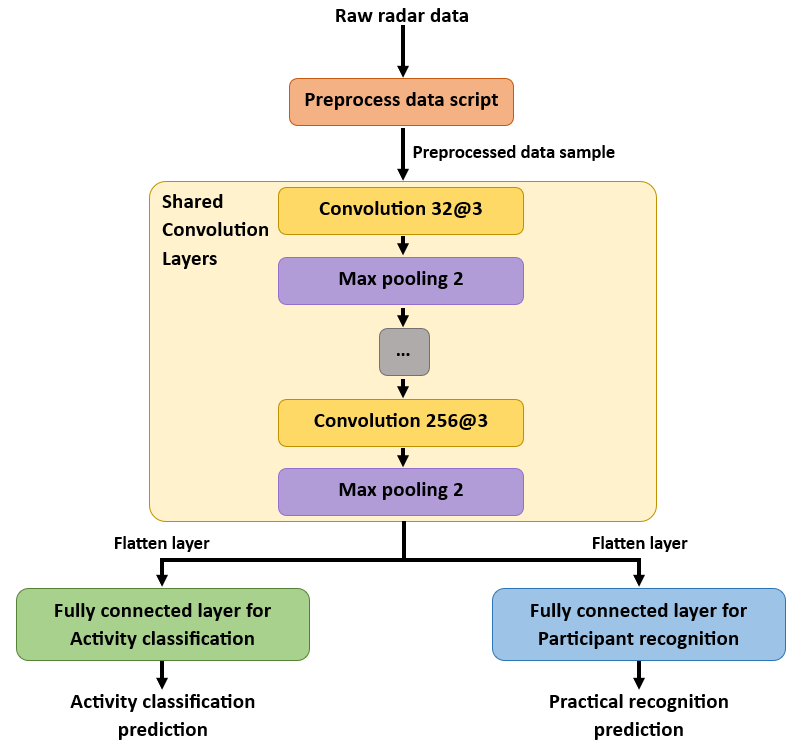
\includegraphics[width=0.7\linewidth]{images/multi-task-model-detailed.png}
    \caption{The multi-task diagram flow utilizes shared feature extraction layers before passing into a flatten layer then splitting into its own fully connected layers for activity classification and participant recognition.}
    \label{fig:multi-task-model}
\end{figure}

\subsection{Privacy Preservation}
\subsubsection{Threat Model:}
In this study, we focus on a scenario taking place within a healthcare central system server, which utilizes Frequency-Modulated Continuous-Wave (FMCW) radar devices to monitor the daily activities of patients. These patients, or participants, are monitored through the radar data captured while they engage in various activities as part of their daily lives. The central system server houses a database that stores these captured radar data. Embedded within this system are two trained models designed to analyze the data: the activity classification model and the participant identification model. These models serve to detect any movement anomalies in the patients, thereby monitoring patients' health and well-being round the clock.

In the method of attack, the scenario unfolds by the attacker gaining unauthorized access to the database of the healthcare central system server, which stores the radar data activities of the patients. This unauthorized access could be achieved through several means, including exploiting system vulnerabilities, leveraging stolen credentials, or even insider threats. We assume that the attacker possesses a trained multi-task model, constructed using the background knowledge of the patients. The model has the capability to predict both activity classification and participant label. Once inside the system, the attacker utilizes the trained multi-task model to identify participant labels for malicious purposes. Given the scenario, the purpose of the study is to design a privacy-preservation mechanism to safeguard participants from the assumed threat. The threat model scenario can be viewed in Figure \ref{fig:threat-model} below.

\begin{figure}[h]
    \centering
    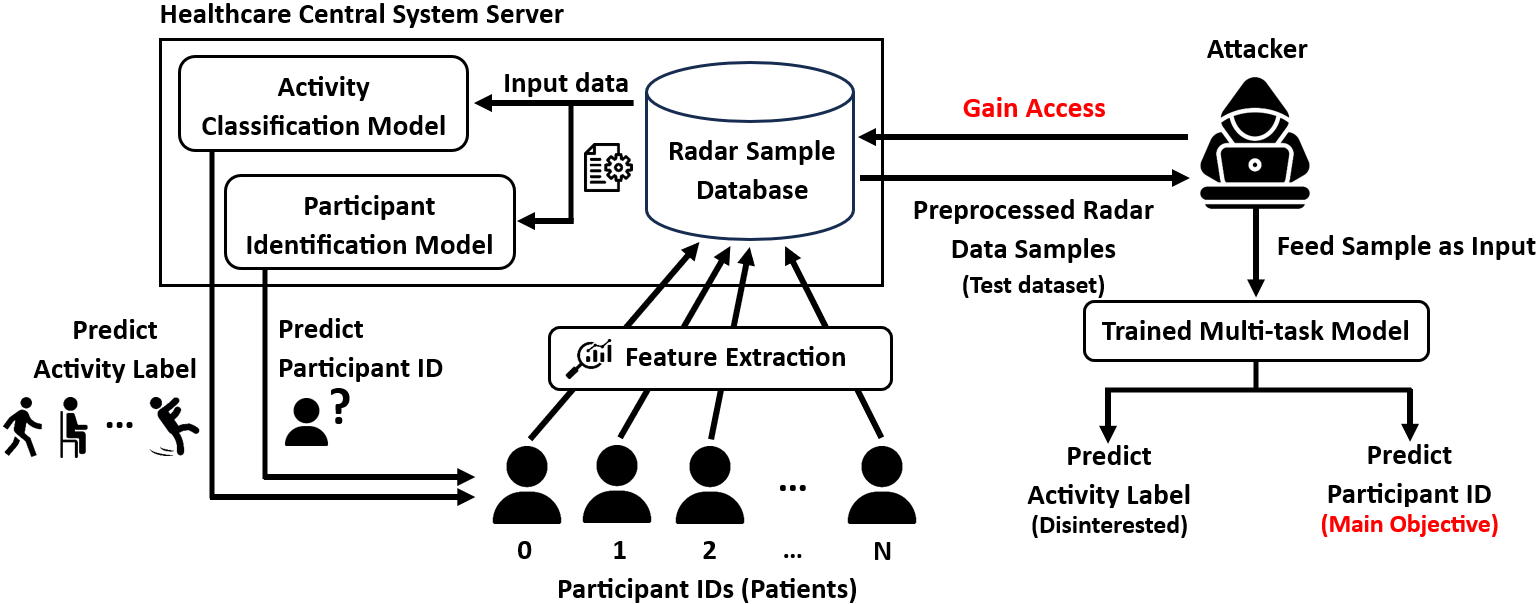
\includegraphics[width=0.9\linewidth]{images/threat-model.png}
    \caption{The threat model for testing privacy preservation mechanism. The attacker's goal is to know the participant IDs for all the (test) data samples stored in database of the healthcare central system server.}
    \label{fig:threat-model}
\end{figure}

\subsubsection{Threat Attack Type:}
The attack in the scenario is based on Model Inversion Attack \citep{model_inversion_attack_analysis}. These attacks exploit the information learned by the model during its training process to infer sensitive attributes, posing a significant privacy risk. By designing a privacy-preservation mechanism to protect against this type of attack, we could also inherently provide protections against a few other related attacks, such as membership inference and model extraction attacks. The former seeks to determine whether a specific data record was used in the model's training set. The latter leverages the output predictions to replicate the deep learning model parameters. In theory, by adding a privacy-preservation mechanism that obscures the relationship between data points and model predictions, the model can reduce the risk of such attacks.

\subsubsection{Privacy Requirement Indicator:}
Our objective is to devise a method that effectively reduces participant identification accuracy without significantly compromising activity classification performance. We must address the privacy requirements necessary to ensure participant protection. Similar to \cite{differential_privacy_with_weighted_privacy_preservation}'s research on preserving privacy of smartphone sensors, for this study, we define privacy success as reducing the identification accuracy to be equal or below the probability of guessing the participant label correctly by chance. Essentially, if the use of the deep learning model results in a lower chance of predicting participant labels accurately, then an attacker might as well resort to guessing. Further details will be discussed in the following chapter.

\subsubsection{Privacy Preservation Mechanism Design:}
There is a few privacy preservation mechanisms in which we can consider, such as downsampling \citep{privacy-preservation_using_low_resolution_depth_images, privacy_preserving_for_extreme_low_resolution}, homomorphic encryption \citep{crypto-nets_neural_network_over_encrypted_data}, and minimax optimization \citep{privacy_preserving_adversarial_framework}. However, in this study, we will investigate deeply into a data obfuscation concept called Differential Privacy (DP) to address the given threat scenario. DP is a privacy-preserving technique that aims to protect sensitive information by adding noise into the data \citep{differential_privacy}. This noise ensures that individual data points cannot be distinguished, thus safeguarding privacy of individuals. While DP enhances privacy, studies have shown that there is utility degradation caused from introducing noise, which reduces the accuracy for other classification tasks as well \citep{algorithmic_foundations_of_differential_privacy, limits_of_differential_privacy_and_its_misuse, tradeoff_between_dp_and_utility}. Subsequently, we will explore modifications to the DP mechanism aimed at optimally preserving privacy while maintaining the usefulness of the data. This exploration led to the development of our proposed mechanism, Adaptive Feature-based Perturbation (AFP).


%==================================================================================================================================
\chapter{Implementation}
In this chapter, we will discuss the steps and technical decisions made to implement the idea outlined in the previous chapter. The description will also involve the discussions of algorithms and techniques that were used.

\section{Radar Dataset}
Throughout the course of the project, we made use of a preexisting radar dataset that has been taken during a research by \cite{RadarSensingForHealthcare}, from James Watt School of Engineering, University of Glasgow. It is to provide the research community with a set of data to build and assess feature extraction and classification algorithms for assisted living, such as detecting falls or anomalies in human motion patterns. Furthermore, this dataset was used for the school's Radar Challenge back in 2020 \citep{radar_challenge_university_of_glasgow}.

Six distinct actions were given to the participants to complete in two to three repetitions: walking back and forth, sitting down on a chair, standing up, bending down to pick up an object, drinking from a glass, and falling frontwards. They were instructed to complete each task independently of one another in separate instances. For some participants, the simulated frontal fall was not recorded due to safety considerations. Moreover, the fall could only be done under certain controlled laboratory conditions.

\subsection{Data Collection Device}
The information was gathered using a Frequency Modulated Continuous Wave (FMCW) radar, manufactured by Ancortek. This device operates at C-band (5.8 GHz) with a bandwidth of 400 MHz and a chirp duration of 1ms. Additionally, it produces an output power of approximately +18 dBm. The radar is linked to Yagi antennas for transmission and reception, each having a gain of around +17dB. Hence, it has the capability to capture micro-Doppler signatures of participants in motion within the area of interest. Figure \ref{fig:raw_data_plots} in the appendix shows six raw data plots, one for each activity, captured by the device. In the plots, the x-axis represents the sample index (position of data collected over time), and the y-axis represents the radar signal magnitude.

\subsection{Data Detail}
The experiments were carried out seven times over the years, spanning from 2017 to 2019. Cumulatively, these experiments involved a total of 106 participants and 1752 radar sample files. The participants ranged in age from 21 to 88 and included both males and females, with an estimated gender ratio of 2:1. Table \ref{tab:dataset-details} and Figure \ref{fig:full-dataset-information}, in the appendix, provides a summary of these details. The files, stored as $.dat$ files, are organized in folders named according to the date of recording. Further information on the dataset can be found in the documentation provided by \cite{IntelligentRFSensing} and \cite{Radarsignaturesofhumanactivities}.

\section{Data Preprocessing}
Even though feature engineering has become less critical with the advent of deep learning, preprocessing of data remains a vital step in model training. Data preprocessing, such as normalization, is essential to ensure that the input data is in a form that deep learning models can easily process. By doing so, data preprocessing can help in accelerating the convergence of the model during training, enabling the model to generalize better to unseen data, and simplifying data complexity to reduce the computational power needed while training.

The radar dataset provided by the University of Glasgow comes with a pre-existing radar preprocessing script written in MATLAB, as documented by \cite{radar_sensing_for_healthcare}. Consequently, the data preprocessing steps we adopted closely align with those outlined in the script. However, we recreated these steps in Python using the NumPy library to facilitate our study analysis.

\subsubsection{1. Data Loading and Reshaping:}
First, the collected data are loaded into the script to convert its data into complex numbers. Next, the relevant parameters are extracted from the radar data, such as center frequency, sweep duration, number of time samples, and bandwidth. Then, the data are reshaped into 2D arrays representing the chirps over time, following column-major order.

\subsubsection{2. MTI Filtering:}
Moving Target Indication (MTI) filter is then used to suppress stationary clutter in the collected data. First, Fast Fourier Transform (FFT) is applied across the time dimension to obtain frequency-domain representation. Range profiles, which are the radar signal's amplitudes corresponding to the participant's distance, are then extracted from the domain. Lastly, an Infinite Impulse Response (IIR) high-pass filter is applied to each range profile using $lfilter()$ from the SciPy library with coefficients obtained from using a high-pass Butterworth filter with a cutoff frequency of 0.0075. Figure \ref{fig:Range-Sweep Plots} displays six range-time plots after applying MTI filter. In the figure, the x-axis represents the number of sweeps, and the y-axis represents the range bins. A radar sweep refers to a single cycle of the radar’s signal transmission and reception. The color in the graph represents the amplitude of the received signal. Hence, the range-time plots have the ability to analyse how the received signals change over both time and distance. 

\begin{figure}[h]
   \centering
   \begin{subfigure}[b]{0.32\textwidth}
        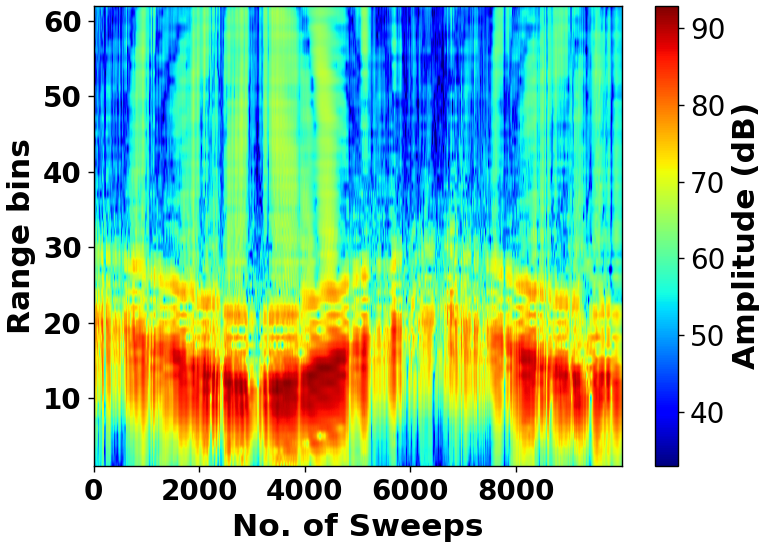
\includegraphics[width=\textwidth]{images/Range-Sweep_1.png}
        \caption{Walking}
        \label{fig:range-sweep1}
    \end{subfigure}
    \hfill
    \begin{subfigure}[b]{0.32\textwidth}
        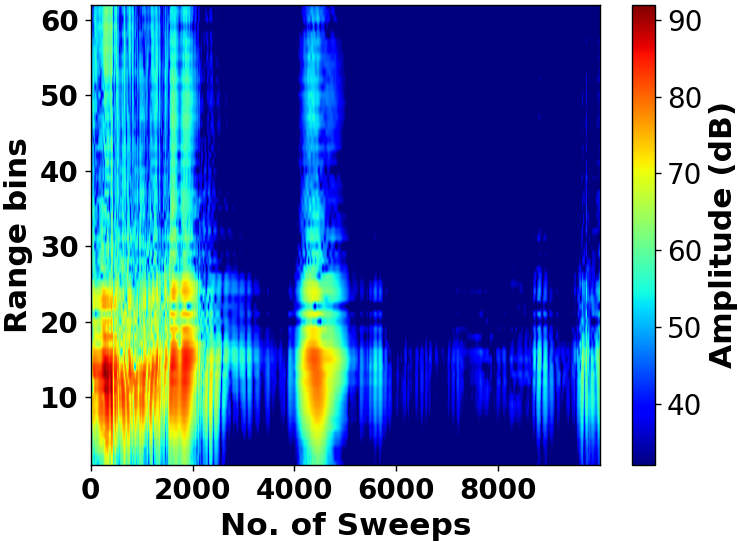
\includegraphics[width=\textwidth]{images/Range-Sweep_2.png}
        \caption{Sitting down}
        \label{fig:range-sweep2}
    \end{subfigure}
    \hfill
    \begin{subfigure}[b]{0.32\textwidth}
        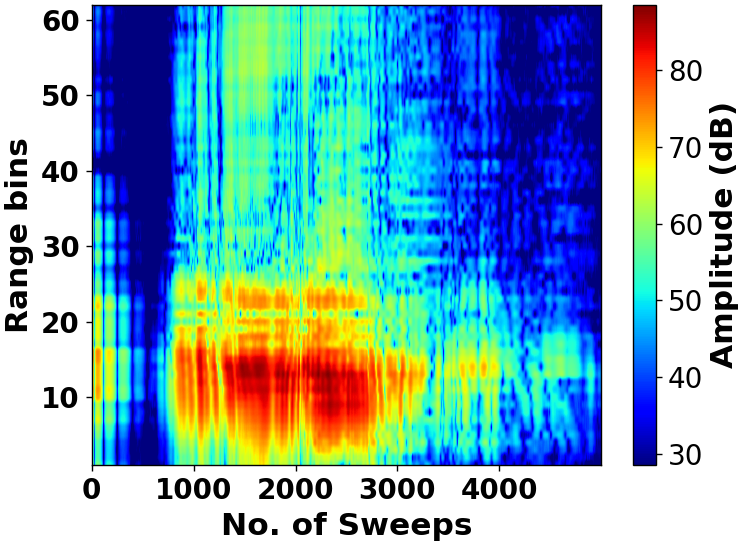
\includegraphics[width=\textwidth]{images/Range-Sweep_3.png}
        \caption{Standing up}
        \label{fig:range-sweep3}
    \end{subfigure}
    \hfill
    \begin{subfigure}[b]{0.32\textwidth}
        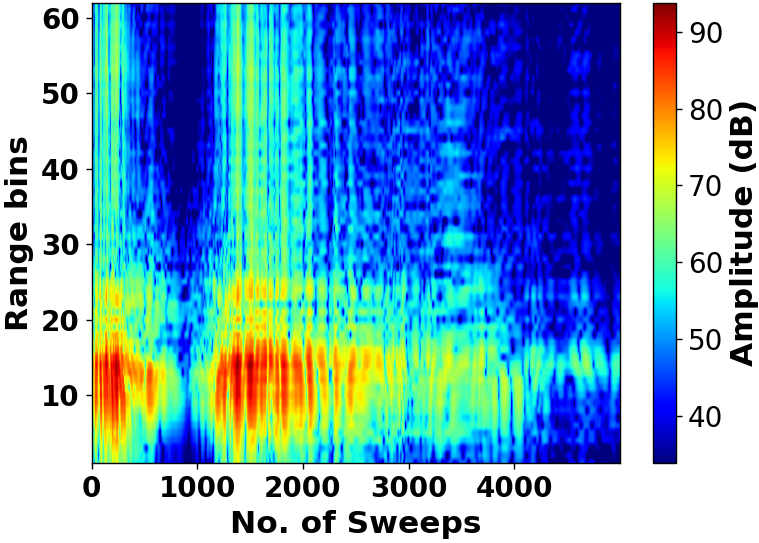
\includegraphics[width=\textwidth]{images/Range-Sweep_4.png}
        \caption{Picking up an object}
        \label{fig:range-sweep4}
    \end{subfigure}
    \hfill
    \begin{subfigure}[b]{0.32\textwidth}
        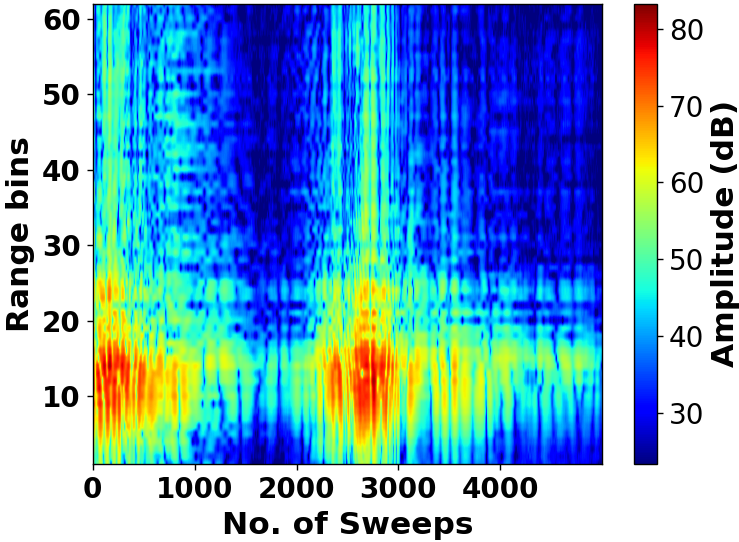
\includegraphics[width=\textwidth]{images/Range-Sweep_5.png}
        \caption{Drinking from a glass}
        \label{fig:range-sweep5}
    \end{subfigure}
    \hfill
    \begin{subfigure}[b]{0.32\textwidth}
        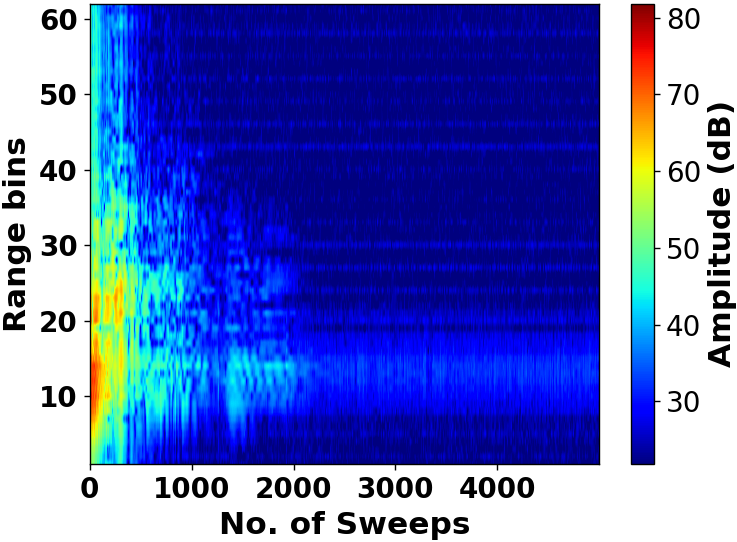
\includegraphics[width=\textwidth]{images/Range-Sweep_6.png}
        \caption{Falling frontwards}
        \label{fig:range-sweep6}
    \end{subfigure}
  \caption{Range-Time plots in the representation of number of sweeps for each of the six activities.}
  \label{fig:Range-Sweep Plots}
\end{figure}

\subsubsection{3. Spectrogram Processing:}
Spectrograms are computed using the $spectrogra()$ function for each range bin of the MTI filtered radar data. A spectrogram provides a 2D representation of how the frequency content of a signal changes over time. Afterwards, $fftshift()$ function is applied to center the frequency axis before applying log scaling to emphasize weaker signals and improve visualization. Figure \ref{fig:Velocity-Time Plots} displays the same radar data but as velocity-time plots, which undertook from applying spectogram processing.

\begin{figure}[h]
   \centering
   \begin{subfigure}[b]{0.32\textwidth}
        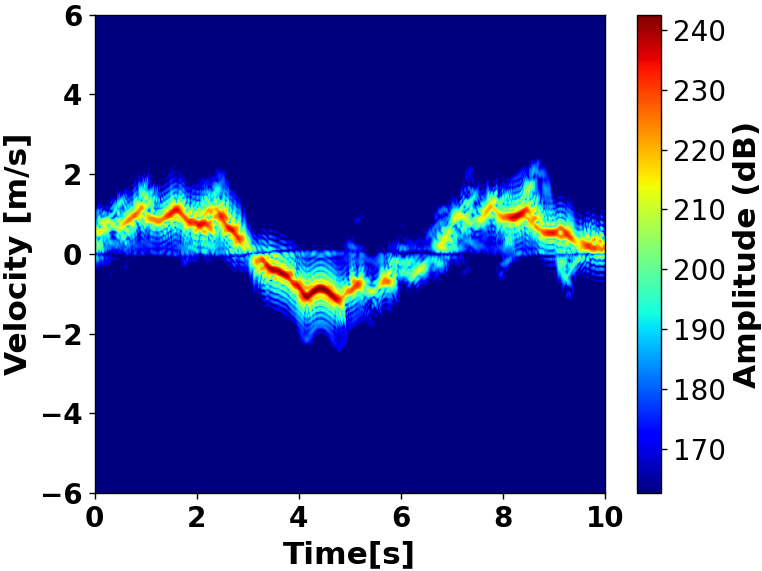
\includegraphics[width=\textwidth]{images/Velocity-Time_1.png}
        \caption{Walking}
        \label{fig:velocity-time1}
    \end{subfigure}
    \hfill
    \begin{subfigure}[b]{0.32\textwidth}
        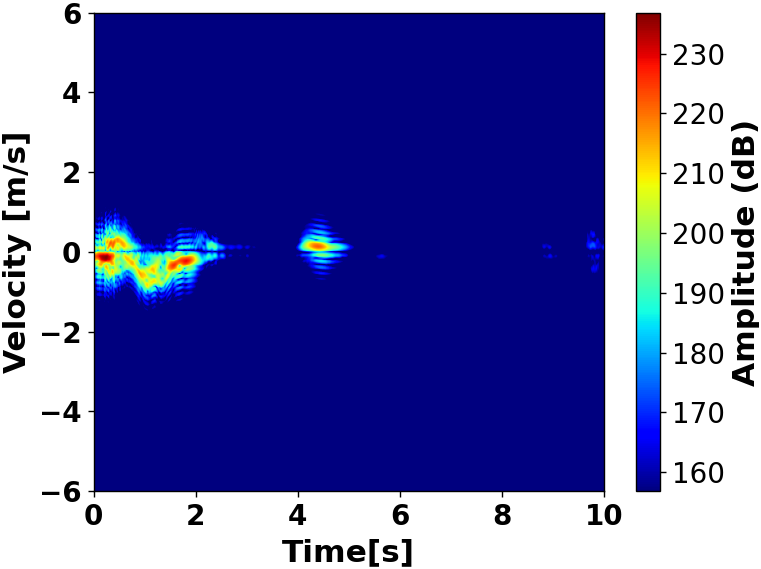
\includegraphics[width=\textwidth]{images/Velocity-Time_2.png}
        \caption{Sitting down}
        \label{fig:velocity-time2}
    \end{subfigure}
    \hfill
    \begin{subfigure}[b]{0.32\textwidth}
        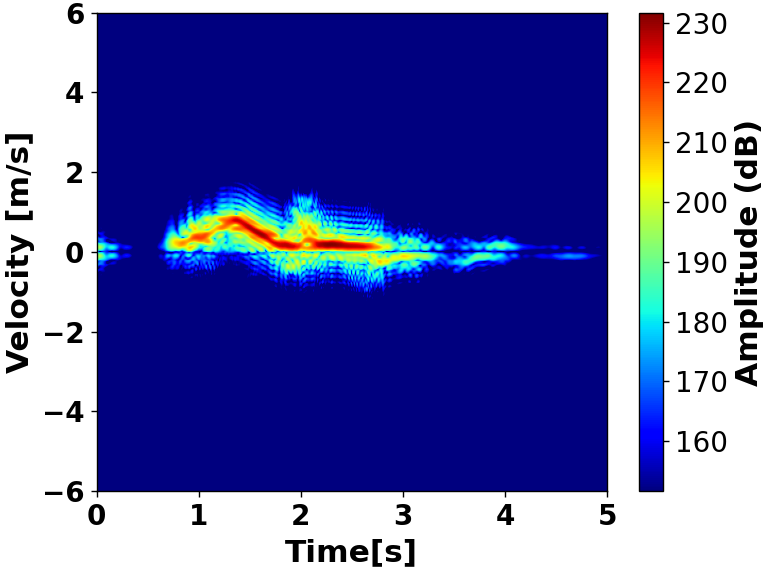
\includegraphics[width=\textwidth]{images/Velocity-Time_3.png}
        \caption{Standing up}
        \label{fig:velocity-time3}
    \end{subfigure}
    \hfill
    \begin{subfigure}[b]{0.32\textwidth}
        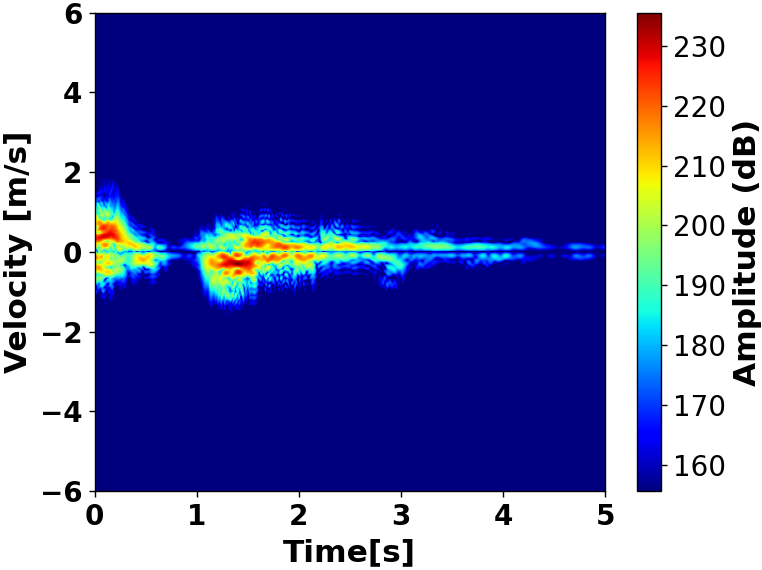
\includegraphics[width=\textwidth]{images/Velocity-Time_4.png}
        \caption{Picking up an object}
        \label{fig:velocity-time4}
    \end{subfigure}
    \hfill
    \begin{subfigure}[b]{0.32\textwidth}
        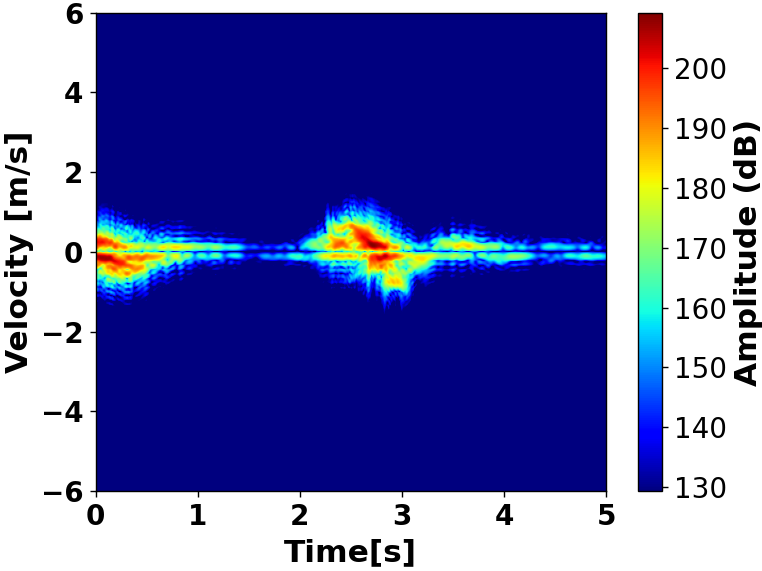
\includegraphics[width=\textwidth]{images/Velocity-Time_5.png}
        \caption{Drinking from a glass}
        \label{fig:velocity-time5}
    \end{subfigure}
    \hfill
    \begin{subfigure}[b]{0.32\textwidth}
        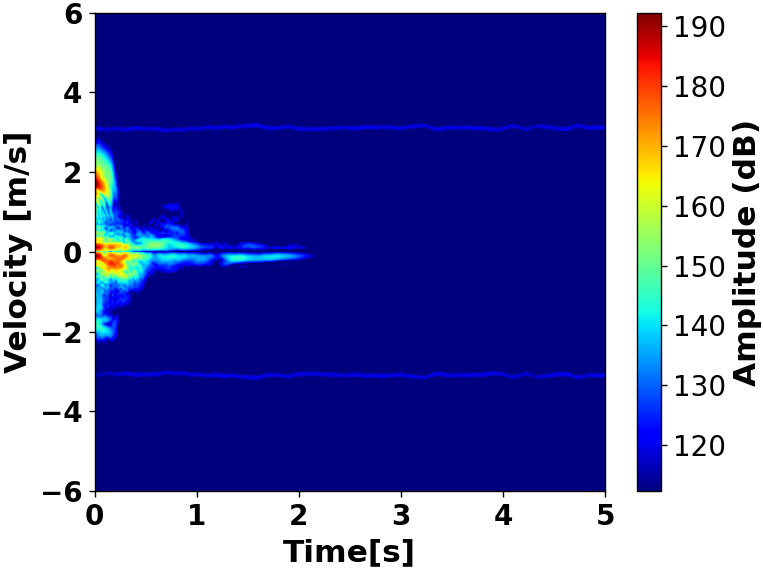
\includegraphics[width=\textwidth]{images/Velocity-Time_6.png}
        \caption{Falling frontwards}
        \label{fig:velocity-time6}
    \end{subfigure}
  \caption{Velocity-Time plot for each of the six activities. These plots are obtained after apply spectrogram processing.}
  \label{fig:Velocity-Time Plots}
\end{figure}

\subsubsection{4. Normalisation and Resizing:}
After we have got the spectrogram representation, we want to implement normalization and resize the data. Normalization is used to ensure that the data is within a consistent range. We would also want to resize the preprocessed data to a lower resolution due to limited computer resource we have available. After resizing, we were able to reduce the data array size from 800x981 to 400x240. Furthermore, we also converted the data type from $float64$ to $float32$. This enables us to decrease the data size 16 times of its original size. Due to resource constraint, these two features are beneficial as they can decrease the time and computational power needed to train the models. Figure \ref{fig:Normalized Resized Comparison Plots} in the appendix shows a before and after comparison of walking activity that has been normalized and resized.

\subsection{Data Filtering} \label{data_filtering}
According to Table \ref{tab:dataset-details} and Figure \ref{fig:full-dataset-information}, it is evident that not all 106 participants were fully involved in the radar data collection process. The variability in participation and activity completion potentially compromises the adequacy of data for training the participant identification models, as a sufficient amount of data is necessary to divide into training, validation, and test sets for each participant to ensure that each of them is represented across all sets.

Ideally, each participant would have 18 recorded radar files, correlating to six activities with up to three repetitions each. However, there were discrepancies in the number of files recorded of some participants, highlighting the challenge. To address this, we filtered out participants that do not have the ideal number of data, narrowing down to 61 participants from the initial 106 participants. Consequently, these 61 participants each contributed 18 radar files, resulting in a total of $61 \times 18 = 1098$ files for our refined dataset. To note, the dataset comprising 106 participants was still utilized for training activity classification models, but not the participant identification models.

\subsubsection{Further Reduction to 30 Participants:}
Having refined our dataset to 61 participants, we sought to create a more manageable dataset size for experimenting with participant identification training. We further reduced the dataset to only 30 participants, yielding a total of $30 \times 18 = 540$ radar files. This selection was made randomly from the 61 participants to ensure fairness. This smaller dataset will serve as the primary basis for evaluating the effectiveness of our trained models, particularly in assessing the impact of the proposed privacy preservation mechanisms later in the project. Importantly, while we focused on the 30-participant dataset later on in the study for detailed evaluations, we also conducted experiments on participant identification model training using the larger dataset of 61 participants. This approach allowed us to compare the model's performance across datasets of different sizes, enriching our understanding of its scalability and robustness in varying contexts.

\section{Data Augmentation} \label{data_augmentation}
Data augmentation is a technique used to artificially increase the size of dataset by applying transformations to the existing data. The primary advantage is to improve generalization and prevent overfitting of the models by having wider range of variations. In this section, we will show two main data augmentation techniques used during training: Axis-flipping and Mixup augmentation.

\subsection{Axis-flipping}
This data augmentation involves flipping the data along its x-axis, y-axis, and on both axes. Horizontal flipping can aid in learning invariant features across horizontal orientations, beneficial for tasks with variable object orientation. Similarly, vertical flipping can aid in capturing variations in vertical symmetry. Diagonal flipping combines x and y-axis flipping, introducing even more variations for the model to learn from. This enables the model to learn from a more comprehensive set of transformations to reduce overfitting and enhance its capability to handle unseen scenarios.

Algorithm \ref{alg:axis-flipping_augmentation}, in the appendix, demonstrates the implementation of axis-flipping augmentation. Horizontal flipping is achieved using the $fliplr()$ function from the Numpy library. Similarly, vertical flipping is conducted with $flipud()$ function, while diagonal flipping combines both methods. Subsequently, the augmented data is concatenated with the original dataset to create a larger dataset. Data labels are also concatenated with the original labels to maintain consistency. Figure \ref{fig:Axis-flipping Plots}, in the appendix, illustrates the application of axis-flipping augmentation on walking data. The figure includes horizontal, vertical, and diagonal flipped data plots.

\subsection{Mixup Augmentation}
Mixup augmentation is a technique used to create synthetic data samples by linearly interpolating pairs of input samples and their corresponding labels \citep{mixup_beyond_empirical_risk_minimization}. For each pair of samples and labels, mixup generates a new sample by blending the features and labels together. This technique blends information from multiple samples, mitigating overfitting and encouraging the model to learn more robust and generalizable representations.

Algorithm \ref{alg:mixup_data_augmentation}, in appendix, demonstrates the logic behind $mixup\_data()$ function. It first computes a mixing coefficient, lambda, using a Beta distribution parameterized by alpha. Then, it randomly shuffles the indices of the batch, to pair samples with each other. For each pair, it creates a new sample and label by linearly interpolating between the original samples and labels based on lambda. 

Figure \ref{fig:mixup_augmentation}, in the appendix, provides a visual representation of mixup augmentation. It takes a pair of radar samples and apply linear interpolation to blend the samples into a new, synthesized sample. This process encourages the model to learn from diverse combinations of data, promoting smoother decision boundaries and better generalization.

\section{CNN Model Implementation}
In the study, we utilized the TensorFlow library to implement and train our Convolutional Neural Network (CNN) models. TensorFlow is a free and open-source software library specifically used for Machine Learning (ML) and Artificial Intelligence (AI). It was developed by the Google Brain team for AI research and production.

\subsection{CNN Layers}
To implement our CNN model, we first load the preprocessed radar samples and shuffle their order to introduce randomness. The training dataset is then fed into the $tf.keras.models.Sequential()$ function to construct the model. This function from TensorFlow organizes the CNN layers, including both feature extraction and classification layers, in a linear stacking sequence. The configuration of CNN layers within the $Sequential()$ function is determined based on our specific requirements. The types of CNN layers employed in this study includes $Conv2D()$, $MaxPooling2D()$, $Flatten()$, $Dense()$, and $Dropout()$ layers.

\subsubsection{Convolution Layer:}
Convolution layer, denoted as $Conv2D()$, is the core building block of CNN architectural design. The layer accepts the number of filters and kernel size as its main parameter. The layer applies the number of filters to the input image to create a feature map. Each filter detects spatial features such as edges, colors, or textures by performing a convolution operation, sliding over the input data and producing a feature map that emphasizes specific aspects detected in it. The size of the sliding window, or filter mask, is determined by the kernel size. Other optional parameters like stride and activation could be set. The former controlling the sliding steps of the kernel and the latter is a type of function that calculates the output of a node based on the subsequent node inputs and their weights.

\subsubsection{Pooling Layer:}
The pooling layer plays a vital role in the downsampling of data, reducing the spatial dimensions (height and width) of the input volume before it reaches the next CNN layer. This reduction is essential for managing the model's computational complexity while ensuring the retention of important features within the data. There are two primary types of pooling layers: Max Pooling ($MaxPooling2D()$) and Average Pooling ($AveragePooling2D()$). The max pooling layer works by retaining only the maximum value of each region of the feature map. This ensures that the most prominent features are emphasized, enhancing the feature map's clarity even after downsampling. In contrast, average pooling smooths the feature map by calculating the average value across each region, maintaining a generalized representation of the features.

\subsubsection{Flatten Layer:}
The Flatten layer, represented as $Flatten()$, serves a pivotal role in transforming the output of the pooled feature maps, which are multi-dimensional arrays, into a one-dimensional array. This transformation is crucial during the transition from the feature extraction phase to the classification phase of the model, which is comprised of fully connected layers. The process of data flattening is essential because fully connected layers require inputs to be in a one-dimensional format to process them effectively.

\subsubsection{Fully Connected Layer:}
A dense layer, indicated as $Dense()$, functions as a fully connected layer where every input node is linked to every output node. It requires specifying the number of nodes and the type of activation function as parameters. This layer handles the flattened input by conducting weighted sum calculations, which are then followed by the application of an activation function. This operation can be depicted by the formula presented in Equation \ref{eq:neuron_activation_function} below. Moreover, a dense layer is commonly utilized for generating the final predictions of the network.
\begin{equation}
    f(b + \sum_{i=1}^{n} x_i \cdot w_i)
    \label{eq:neuron_activation_function}
\end{equation}
\textit{\textbf{Equation~\ref{eq:neuron_activation_function}:} The equation of neuron activation function represents how the inputs to a single neuron is transformed into an output signal.
$b$ is the bias, $w$ is the weight, $x$ is the neuron value, and $f$ is the activation function applied.}

\subsubsection{Dropout Layer:}
The Dropout layer, represented by $Dropout()$, serves as a regularization technique designed to prevent overfitting in neural networks \citep{dropout, dropout2}. This layer accepts a rate, ranging from 0 to 1, as its input parameter. This rate specifies the probability of randomly setting input elements to zero during each update in the training phase. Consequently, this process encourages the model to learn more robust features, fostering greater independence among neurons.

\subsection{Activation Functions}
Activation functions play a crucial role in introducing non-linearity into machine learning models, enabling the network to capture more complex data representations. While numerous activation functions are available, this section focuses on two most utilized in this study: the Rectified Linear Unit (ReLU) and Softmax functions.

\subsubsection{Rectified Linear Unit (ReLU):}
First introduced by \cite{cognitron_self-organizing_multilayered_nn}, ReLU has become the most popular activation function in deep learning models today. As depicted in Figure \ref{fig:ReLU}, the function outputs 0 for any negative input and returns the input itself for any positive value. Despite its simplicity, ReLU is highly effective. Research by \cite{deep_sparse_rectifier_nn} demonstrated that ReLU enables faster and more efficient training of deep neural networks on large and complex datasets compared to other activation functions available at the time. This is due to its ability to facilitate better gradient propagation, mitigating the vanishing gradient problem that previously posed a significant challenge.

\begin{figure}[h]
    \centering
    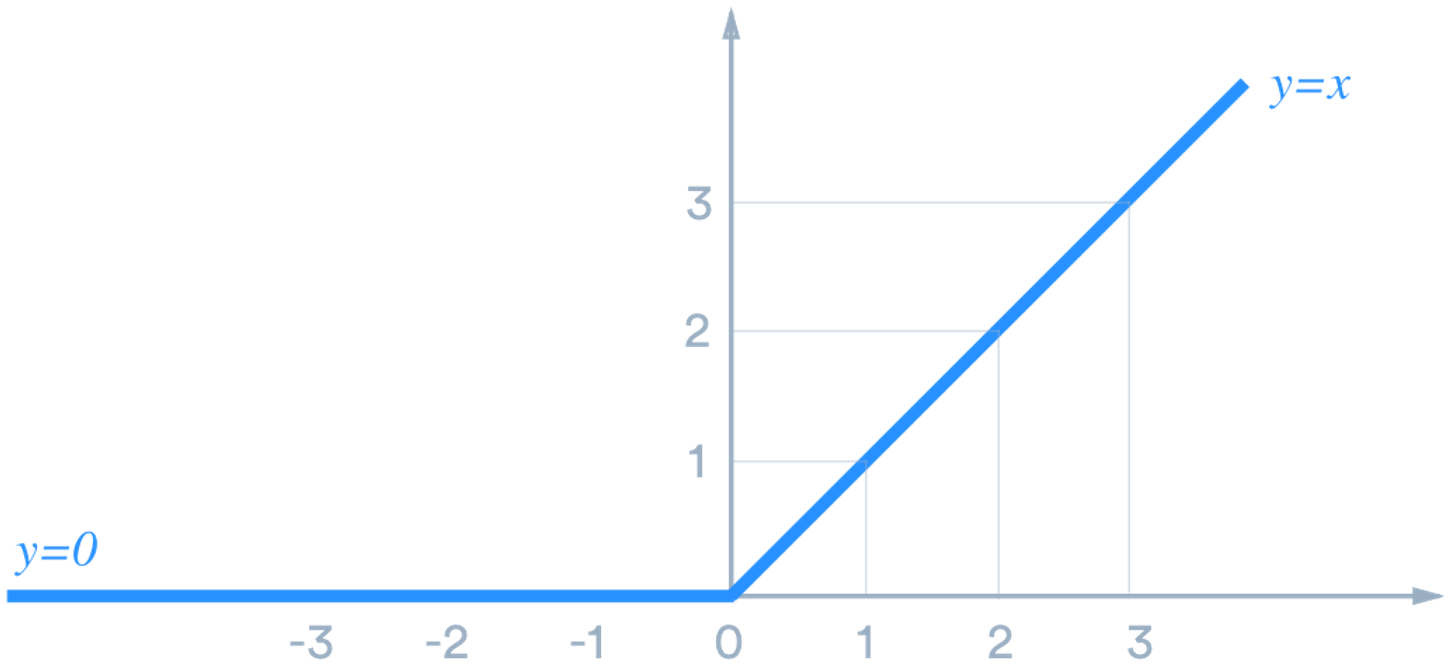
\includegraphics[width=0.5\linewidth]{images/ReLU.png}
    \caption{The figure presents the graph of ReLU activation function. The formula of ReLU can be written as $f(x) = max(0,x)$.}
    \label{fig:ReLU}
\end{figure}

\subsubsection{Softmax Function:}
The softmax function is a widely used activation function when dealing with multi-classification problems. It is typically employed as the final activation function to transform the output vector of a network into a probability distribution across predicted output classes, adhering to Luce's choice axiom \citep{luce_axiom}. After obtaining the probability distribution, we can utilize $argmax()$ function in NumPy to determine the most confident class label prediction of the model.

\begin{figure}[h]
    \centering
    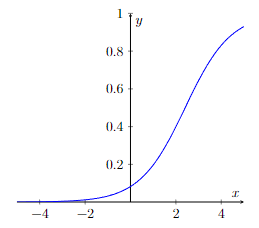
\includegraphics[width=0.35\linewidth]{images/softmax_function.png}
    \caption{The figure presents the graph of Softmax activation function. The equation of the function can be expressed as $\sigma(z_i) = \frac{e^{z_{i}}}{\sum_{j=1}^K e^{z_{j}}}$.}
    \label{fig:enter-label}
\end{figure}

\newpage

\subsection{Loss Function and Optimizer}
Loss functions are methods of quantifying how well the model is performing using numerical representation. They typically measure the discrepancy between the model's predicted outputs and the actual labels, calculating a loss value that indicates the prediction's deviation from the ground truth. The optimizers, conversely, are algorithms that seek to minimise the loss function by taking steps to adjust the model's attributes, such as weights and learning rate, to improve its accuracy. In this section, we will discuss the primary loss function and optimizer employed in our study.

\subsubsection{Cross-Entropy (CE) Loss:}
Cross-Entropy loss function is a popular choice in dealing with multi-class and multi-label classifications. The loss function works by computing the difference between the predicted class probabilities and the true class labels. Advantages of using CE is that it works well when the model outputs are represented as probabilities (output of softmax activation function) and it offers smoother gradients than other loss functions, which can lead to better convergence during training. The mathematical equation of CE can be viewed in Equation \ref{eq:cross_entropy} below.
\begin{equation}
    -\sum_{c=1}^My_{o,c}\log(p_{o,c})
    \label{eq:cross_entropy}
\end{equation}
\textit{\textbf{Equation~\ref{eq:cross_entropy}:} The equation shows mathematical formula of Cross-Entropy loss. $M$ is the number of classes, $y$ is binary indicator of correct classification of class label $c$ for observation $o$, and $p$ is the predicted probability observation $o$ is of class label $c$.}

\subsubsection{Adam Optimizer:}
Adaptive Moment Estimation (Adam) optimization is an extension of the Stochastic Gradient Descent (SGD) algorithm, characterized by its adaptive learning rate adjustments during training. Initially proposed by \cite{adam_optimizer}, Adam is a first-order, gradient-based optimization technique known for its computational efficiency and minimal memory requirements. One of the key benefits of Adam is its ability to reduce the sensitivity to hyperparameter tuning, making it more user-friendly in practice. Furthermore, research by \cite{toward_understanding_of_adam} has demonstrated that Adam can achieve faster convergence compared to SGD. This is attributed to its capability to effectively manage issues related to high directional sharpness by adjusting the step size individually for each parameter, leading to more stable and efficient optimization progress. Given these advantages, the Adam optimizer is well-suited for handling larger datasets and works well in practice when compared to other stochastic optimization algorithms.

\subsection{Hyperparameter Tuning Strategies}
Beyond the implementation settings previously outlined, we also explored hyperparameter tuning strategies within the study, including early stopping and hyperparameter tuning framework.

\subsubsection{Early Stopping:}
We incorporated an early stopping mechanism into the model training process. Early stopping serves as a regularization technique designed to prevent the overfitting of the model. Moreover, early stopping ensures that the model maintains generalization capabilities and does not learn from the noise in the training data. Furthermore, it also makes the training process more efficient by avoiding unnecessary computations once the model has ceased to improve, thereby saving time and computational resources. In the study, we implemented early stopping with a patience parameter of 10, this means that the training process halts if the model fails to decrease the validation loss for ten consecutive epochs. Additionally in Tensorflow, we can set the early stopping function with $restore\_best\_weights=True$, which will retain the best model weights of the training process.

\subsubsection{Hyperparameter Tuning:}
Hyperparameter tuning is a technique for optimizing parameter settings, including learning rate, number of epochs, and batch size, to achieve the best performance when training a model. For hyperparameter tuning, we utilized a framework known as Optuna. Optuna is renowned for its state-of-the-art algorithms that efficiently search the hyperparameter space. It adopts Bayesian optimization with a Tree-structured Parzen Estimator (TPE) algorithm, enabling an iterative process that models the behavior of the objective function. This methodology allows Optuna to effectively guide the search towards the most optimal hyperparameter values, enhancing the model's overall performance. However, due to hardware restrictions in the study, we were not able to utilize Optuna in full. We also conducted manual hyperparameter tuning experiments.

\section{Single-task Model Classification}
\subsubsection{Activity Classification Model:}
The activity classification model is designed to analyze radar signals to classify human activities based on extracted features. The activities to be classified include walking, sitting down, standing up, picking up an object, drinking from a glass, and falling frontwards. Therefore, the size of the one-hot encoding label would be six. The information of how we map the activity labels to their corresponding one-hot encoding array can be view in Table \ref{tab:one-hot_encoding_activity} in the appendix. Figure \ref{fig:activity-classification-model} below illustrate one of the CNN model used during training.

\begin{figure}[h]
    \centering
    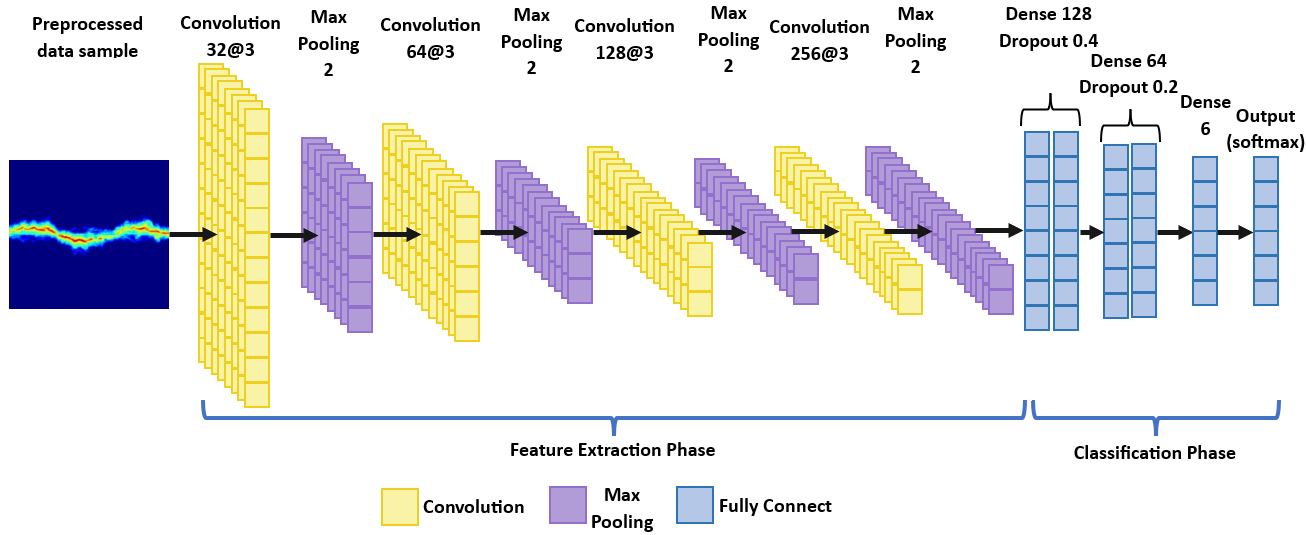
\includegraphics[width=1.1\linewidth]{images/activity-classification-model.png}
    \caption{An example of a CNN network model used during activity classification training.}
    \label{fig:activity-classification-model}
\end{figure}

\subsubsection{Participant Identification Model:}
The participant identification model is designed to classify individuals based on preprocessed radar samples. This process entails training the model to recognize and categorize the unique behavioral activity patterns associated with each participant. Unlike the activity classification model, the participant model is more complex because the size of the one-hot encoding array varies with the number of participants to be classified. This variation is directly influenced by the dataset we employ: 61-participant or 30-participant dataset. Consequently, the size of the one-hot encoding array could be either 61 or 30, depending on the dataset choice. Further detail of the datasets used can be viewed in Table \ref{tab:participant-identification-number-of-samples} of the appendix. Figure \ref{fig:participant-recognition-model} below demonstrates one of the CNN model used during training.

\begin{figure}[h]
    \centering
    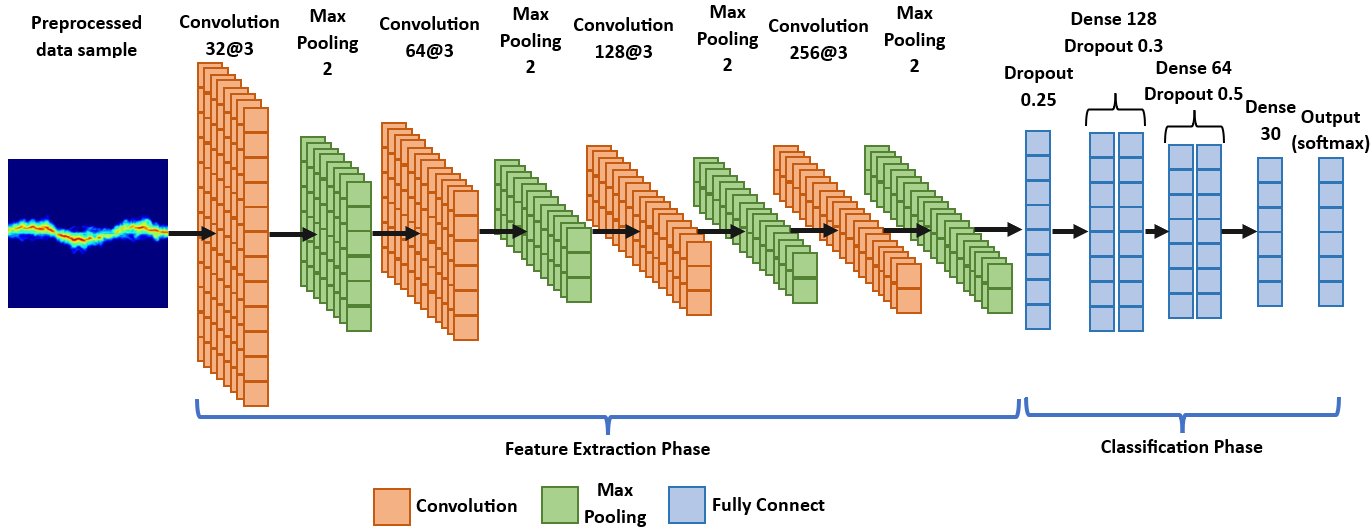
\includegraphics[width=1.1\linewidth]{images/participant-recognition-model.png}
    \caption{An example of a CNN network model used during participant recognition training.}
    \label{fig:participant-recognition-model}
\end{figure}

\section{Multi-task Model Classification}
The similarity of the above single-task model designs facilitates efficient integration, allowing the multi-task model to share a common feature extraction layers before branching into task-specific layers for classification. For the multi-task model in this project, we utilized the shared-bottom multi-task architecture as discussed in the design chapter in section \ref{multi-task_model_design}.

\subsection{Additional Parameter}
Multi-task models are inherently more complex than their single-task counterparts due to the use of shared layers and parameters. A common challenge encountered is the imbalance in task losses, where the loss from one task may overshadow that of another. To mitigate this issue, tuning an additional parameter known as loss weights becomes necessary. Given that our model yields two outputs—one for activity classification and another for participant recognition—consideration of two distinct loss weights, one for each task, is essential. By adjusting the weights associated with each task's loss, our goal is to ensure a balanced contribution from both tasks to the overall loss function. Based on our experiments, setting the loss weight for activity classification at 1.0 and for participant recognition at 8.0 serves as an effective starting point for further experimentation.

\section{Privacy Preservation Mechanism}
As discussed in the design chapter, our selected privacy-preservation technique for investigation is Differential Privacy (DP). DP is a privacy-preserving technique that aims to protect sensitive information within datasets by incorporating noise into the data \citep{differential_privacy}. This added noise helps to obscure individual data points, thereby enhancing the privacy of individuals. However, while DP significantly improves data privacy, multiple research indicates a trade-off between privacy and utility due to the introduction of randomness \citep{algorithmic_foundations_of_differential_privacy, limits_of_differential_privacy_and_its_misuse, tradeoff_between_dp_and_utility}. This trade-off can adversely affect the prediction accuracy of classification tasks.

\subsection{Privacy Requirement} \label{privacy_requirement}
Based on the threat model depicted in Figure \ref{fig:threat-model}, our goal is to protect the identities of participants while preserving the utility of activity classification. Therefore, it is crucial to establish a privacy requirement that gauges the success of mitigating the identified attack, ensuring effective participant protection. Drawing inspiration from \cite{differential_privacy_with_weighted_privacy_preservation}'s research on privacy preservation in smartphone sensors, our study defines success in mitigating the attack as limiting participant identification performance to equal to or less than the probability of correctly guessing the participant label by chance. Hence, our privacy requirement indicator can be calculated as follows: 
\begin{equation}
    f(x) = \frac{1}{x}\: \text{; x = Number of Participants in the Dataset}
    \label{eq:privacy_requirement_indicator}
\end{equation}
Since we used the 30-participant dataset for our privacy evaluation, the privacy indicator can be computed as:
\begin{align*}
    Privacy\: Indicator = \frac{1}{\text{Number of Participants}} = \frac{1}{30} = 0.03\dot{3} = 3.33\%
\end{align*}
To achieve this objective, we implemented Adaptive Feature-based Perturbation (AFP) as our proposed privacy-preserving mechanism based on the Laplace mechanism and $\epsilon$-differential Privacy ($\epsilon$-DP). In preparation for introducing our AFP mechanism, we will first aim to provide an overview of the Laplace mechanism and the concept of $\epsilon$-DP.

\subsection{Laplace Mechanism}
The Laplace mechanism is a fundamental technique in DP, employing a technique known as Laplace noise to randomize the output of a function, thereby safeguarding privacy. This noise is derived from the Laplace distribution, characterized by its probability density function as shown in Figure \ref{fig:laplace-distribution}. A key feature of this distribution is its scale parameter ($b$), which directly influences the distribution's peak sharpness and the rate at which the probability density decreases exponentially away from the center. A smaller $b$ value results in a steeper peak, ensuring that the added noise is finely tuned to the sensitivity of the function being protected and the desired privacy level ($\epsilon$), without unnecessarily degrading data utility.

Unlike the Gaussian distribution, which is characterized by its bell-shaped curve, the Laplace distribution has heavier tails. This attribute of the Laplace distribution is particularly advantageous in the context of $\epsilon$-differential privacy guarantees. The heavy tail characteristic adheres to a stricter privacy requirement, making it more effective in protecting highly sensitive features that require substantial obfuscation. In contrast, the Guassian distribution is often used for ($\epsilon,\delta$)-differential privacy, where a small probability of privacy failure ($\delta$) is deemed acceptable, due to its different tail behavior.

\begin{figure}[h]
    \centering
    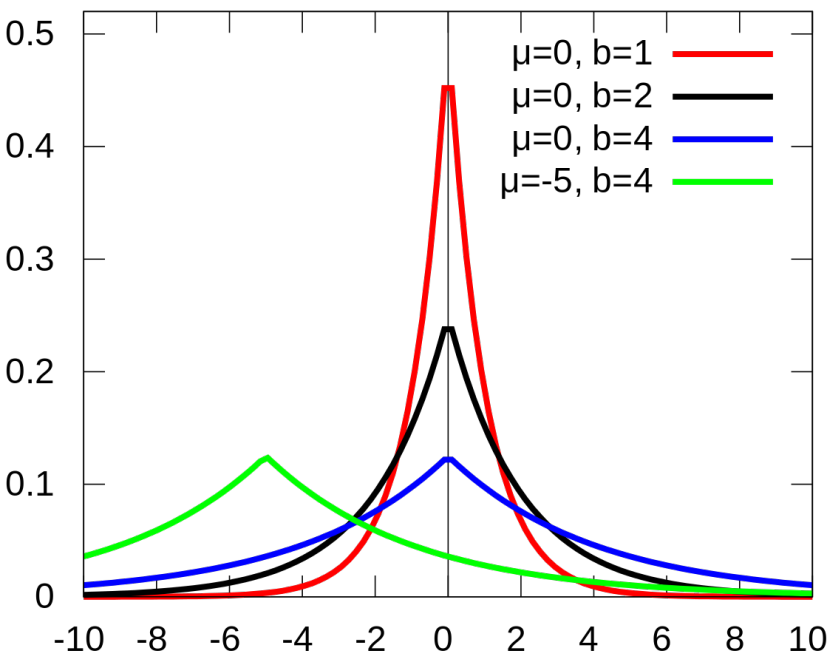
\includegraphics[width=0.33\linewidth]{images/laplace-distribution.png}
    \caption{The figure shows the Laplace distributions when applied with different parameters. $b$ represents the scale parameter, controlling the spread or width of the Laplace distribution, while $\mu$ denotes the location parameter, specifying the mean of the distribution.}
    \label{fig:laplace-distribution}
\end{figure}

\subsection{$\epsilon$-differential Privacy} \label{epsilon_dp}
First introduced by \cite{differential_privacy}, $\epsilon$-differential Privacy ($\epsilon$-DP) is a privacy framework developed to protect sensitive data. It takes the concept of randomized mechanism to ensure privacy against all attacks. The definition of the randomized mechanism $M$ can be written as follows \citep{bootstrap_dp}:
\vspace{0.1cm}
\newline
\textbf{Definition 1:} A randomized mechanism $M$ satisfies $\epsilon$-differential privacy if for all neighboring datasets $x, y \in U^n$, and all measurable $S \subseteq \text{Range}(M)$, we
have:
\begin{equation}
    \Pr(M(x) \in S) \leq e^{\epsilon} \times \Pr(M(y) \in S)
    \label{eq:randomized-M_dp}
\end{equation}
The mechanism introduces $\epsilon$ as a privacy parameter signifying the privacy strength added to the data. According to the definition, if the privacy-preserving mechanism $M$ satisfies $\epsilon$-DP, smaller $\epsilon$ values indicate stronger privacy guarantees, leading to the addition of more noise. Conversely, larger $\epsilon$ values reduce privacy by injecting less noise but enhance utility. The algorithmic representation of applying $\epsilon$-DP can be seen in Algorithmic \ref{alg:laplace_mechanism}, in the appendix. 

\subsection{Adaptive Feature-based Perturbation (AFP)} \label{adaptive_feature-based_perturbation}
Our proposed privacy-preservation mechanism, AFP, is based on the concept of Laplace mechanism and the DP composition theorem, as described in section \ref{epsilon_dp}. However, our method diverges from standard DP approaches that apply noise across all data attributes. Instead, we focus on adding Laplace noise specifically to the top K features most crucial for identifying participants. The rest of the features in the dataset, represented as $N - K$ where N is the total number of features in the radar data, remain unaltered. This targeted strategy aims to maximize participant privacy preservation while minimizing the impact on the activity classification performance.

\subsubsection{Inversion of $\epsilon$-DP Mechanism:}
We employed a modified approach of $\epsilon$-DP, which represents an inversion of the conventional method as shown in Equation \ref{eq:randomized-M_dp}. This novel strategy reverses the principle, wherein higher values of epsilon ($\epsilon$) indicate higher strength of privacy preservation through the addition of more noise into the data. Subsequently, the smaller the $\epsilon$ is, the less noise is added to the data. Conventionally, the scale parameter of the Laplace distribution is determined by $\frac{1}{\epsilon}$. Therefore, $\epsilon=0$ would result in division by zero and an error. But by adopting the inversion method, we establish a unique interpretation of $\epsilon$, wherein a value of $\epsilon=0$ signifies the absence of noise added to the data.

\subsubsection{Extracting Top K Features:}
Our AFP mechanism adds Laplace distribution noise to the top k features critical for participant identification analysis. In this section, we will delve into two methods of implementation to extract the features ordered by importance.

The first implementation employs the SHapley Additive exPlanations (SHAP) library to calculate SHAP values. SHAP is an effective tool for extracting feature importances, providing insights into predictions made by deep learning models for evaluation. Initially, we utilized the $DeepExplainer()$ function to construct an explainer, inputting the model to be evaluated and the training set as parameters. Subsequently, the $compute_shap_values()$ function is called, with the explainer and the test set as inputs, to compute the SHAP values. Upon obtaining the SHAP values, we averaged them across all test set predictions and used $argsort()$ to rank features by importance. SHAP is considered one of the best methods for feature extraction from deep learning models, as it is explicitly designed for this purpose. However, due to hardware limitations in this study, we were unable to complete the computation of SHAP values due to session crashes. Consequently, we sought an alternative method for conducting feature extractions.

Our alternative solution involved using Random Forest models. The feature importances can be extracted using $feature\_importances()$ attribute from the $RandomForestClassifier$ in the scikit-learn module. Random forest is an ensemble learning method used for classification and regression tasks. It operates by constructing numerous decision trees during training and outputs the classification or regression of the individual trees. Subsequently, the $feature\_importances()$ function computes feature importance by measuring the reduction in impurity (Gini Impurity (GI) and Gini Index) that each feature contributes when making splits within the decision trees. Features that lead to a more significant reduction in impurity are considered more important. The formula of calculating GI is as follows:
\begin{equation}
    \text{Gini Impurity} = 1 - \sum_{i=1}^{n} (P_i)^2 = 1 - [(P+)^2 + (P-)^2]
\end{equation}
Before employing the $feature\_importances()$ function, it is necessary to train our Random Forest model. This can be achieved by feeding the data and the participant labels to the model. Once trained, $feature\_importances()$ can be called. This function returns an array containing the importance scores for all features in a radar sample. These scores indicate each feature's relative contribution to the overall predictive performance of the Random Forest model, with higher scores marking features with a greater impact on the model's predictions. Subsequently, the $argsort()$ function can be  used to conduct an indirect sort, and array slicing can extract the top K most relevant features for participant identification. The exploration to determine the optimal value of K will be discussed in the evaluation chapter.

\section{Differential Privacy Mechanisms For Evaluation}
We have implemented two DP mechanisms for evaluation and comparison:

The first mechanism is the application of the conventional $\epsilon$-DP mechanism which adds Laplace noise distribution to all features in the data. Even though this method ensures strong privacy preservation, it will be later revealed that it also significantly deteriorate the performance of activity classification. This underlines the necessity of modifying the conventional methods of applying DP in order to balance the privacy preservation to still be below the privacy requirement threshold while minimizing the performance deterioration of activity classification, which is the utility. In our implementation, we slightly modified the conventional $\epsilon$-DP mechanism by inverting the relationship between $\epsilon$ and noise strength; thus, a higher $\epsilon$ value corresponds to an increase in the noise added to the data. The algorithmic representation of this can be seen in Algorithmic \ref{alg:laplace_mechanism_inverse}, in the appendix. 

The second mechanism is our proposed AFP mechanism. This involves adding Laplace noise targeted to the top K most crucial features for identifying participants, as discussed in section \ref{adaptive_feature-based_perturbation}. Utilizing our proposed mechanism, we aim to minimize the impact on the performance of the activity classification task while reducing the participant recognition task's effectiveness to be equal to or less than the probability of guessing the participant label correctly by chance, which can be computed as shown in section \ref{privacy_requirement}. The algorithmic representation of applying noise using AFP can be seen in Algorithmic \ref{alg:enhanced_weighted_laplace_mechanism}, in the appendix. The model diagrams of both DP models, the standard $\epsilon$-DP and the proposed AFP, are shown in Figure \ref{fig:differential-privacy-mechanism-models} , in the appendix.

%==================================================================================================================================
\chapter{Evaluation} 
In this chapter, we will present the results of the experiments that were conducted in each phase of the implementation as discussed in the implementation chapter.

\section{Data Splitting Methods}
Data splitting plays a critical role in machine learning, as it involves dividing data samples into subsets for training, validation, and testing purposes. This process is crucial for ensuring that the model is trained effectively and yields reliable and unbiased performance results for evaluation. Within this study, we employed two main methods of data splitting. The first method was initially used during early stages of the study, while the second was introduced to address the shortcomings of the first method.

\subsection{Initial Data Splitting Strategy}
Our initial approach to data splitting involved using the entire radar dataset, which includes data from 106 participants. To start, we manually selected 260 data files to constitute the test set, prioritizing the exclusion of these files from the model's training to ensure they remain unseen. The rest of the data was then divided randomly, allocating 82\% for training and 18\% for validation, approximating a split ratio of 70:15:15 across training, validation, and testing sets, respectively.  This method was applied exclusively during the training phase of the activity classification model. The precise data division is depicted in Figure \ref{fig:data-splitting-method1}, in the appendix.

While this strategy proved effective for training the activity classification model, it encountered significant limitations when applied to participant identification model training. First, not every participant completed the experiment with all activities and repetitions, leading to potential gaps in data representation for some participants in the training, validation, and testing sets. Ideally, each participant would contribute 18 recorded radar files (six activities with three repetitions each). However, as shown in Figure \ref{fig:full-dataset-information} in the appendix, there are noticeable discrepancies in the number of files recorded for certain participants, which complicates the data splitting process. Second, randomizing the dataset as a whole might concentrate all data from some participants into only one or two of the three divisions, thus not providing a balanced representation for model evaluation. It is essential to ensure that there is at least one instance from each participant across all splitting sets to ensure the model is trained, validated, and tested comprehensively for generalization.

\subsection{Refined Data Splitting Strategy}
The second data splitting method was developed to enhance robustness and ensure independence from noise, addressing the challenges encountered with the initial data splitting strategy. This approach leverages the datasets of 61 and 30 participants, refined through the data filtering process described in data filtering section \ref{data_filtering}. Initially, one sample data from each participant is randomly selected for the test set. Following this, four samples from each participant are allocated to the validation set, with the remaining samples are used for the training set. This method guarantees representation from every participant across all sets, thereby ensuring a balanced and comprehensive evaluation framework. This refined approach is employed consistently throughout the study for training both the activity classification and participant identification models, as well as for assessing the impact of Differential Privacy (DP) measures. Figure \ref{fig:data-splitting-method2}, in the appendix, depicts the dataset splitting ratio of the method. It is important to note that, regardless of whether the 61-participant or 30-participant dataset is utilized, the splitting ratio remains consistent.

\section{Metrics for Evaluation}
As our milestones primarily involve training and analyzing Convolutional Neural Network (CNN) models, our selection of evaluation metrics will be based on the following metrics to ensure a comprehensive assessment of the CNN model performances:
\begin{itemize}
    \item \textbf{Accuracy:} This measures the proportion of correctly classified instances among all instances, making it a straightforward and intuitive metric. However, in imbalanced datasets, accuracy might not provide a comprehensive understanding of model performance.
    \begin{equation}
        Accuracy = \frac{True Positive + True Negative}{True Positive + True Negative + False Positive + False Negative}
    \end{equation}
    \item \textbf{Precision:} This is used to quantify the proportion of true positive predictions among all positive predictions, focusing on the correctness of positive predictions.
    \begin{equation}
        Precision = \frac{True Positive}{True Positive + True Negative}
    \end{equation}
    \item \textbf{Recall:} Also known as sensitivity, recall measures the proportion of true positives that were correctly identified by the model, providing insights into the model's ability to capture all positive instances.
    \begin{equation}
        Recall = \frac{True Positive}{True Positive + False Negative}
    \end{equation}
    \item \textbf{F1-score:} F1-score combines precision and recall into a single metric. This is useful for achieving a balance between precision and recall.
    \begin{equation}
        F1-score = 2 \times \frac{Precision \times Recall}{Precision + Recall}
    \end{equation}
\end{itemize}

The accuracy metric will be the only metric in this study expressed as a percentage, ranging from 0 to 100. Precision, recall, and F1-score will be represented on a scale from 0 to 1. Higher values of these metrics indicate better performance, signifying its accuracy in predicting unseen radar data. Accuracy and F1-score will be our primary classification metrics used for evaluation.

\section{Activity Classification Evaluation}
The activity classification task encompasses six possible classes: walking, sitting down, standing up, picking up an object, drinking from a glass, and falling frontwards. The outcomes from training the activity classification models across all dataset types —namely, the full 106-participant dataset, the 61-participant dataset, and the 30-participant dataset— have been quite satisfying. The development process, covering the baseline performance, hyper-parameter tuning, ablation study findings, and the determination of the optimal CNN model configuration, will be elaborated upon in the following sections.

\subsection{Baseline Performance Result} \label{activity_baseline_performance_result}
We begin by presenting the baseline performance results to serve as a reference point for all subsequent evaluations. This approach ensures a consistent and reproducible framework for experimentation and analysis across our studies. The baseline CNN model layer configurations are detailed in Table \ref{tab:activity-initial-CNN-configuration} in the appendix. Additionally, we set the baseline learning rate at 0.0002, with a training duration of 10 epochs and a batch size of 64.

Although the initial results are promising, there is potential for further enhancement. Figure \ref{fig:acitivity-initial-loss-and-accuracy-plots} showcases the train and validation losses and accuracies throughout the training epochs. The similarity in loss and accuracy values between training and validation sets suggests effective learning. However, the absence of convergence indicates that experimenting with an increased number of epochs and an adjusted learning rate might yield improvements.
\begin{figure}[h]
   \centering
   \begin{subfigure}{0.4\textwidth}
        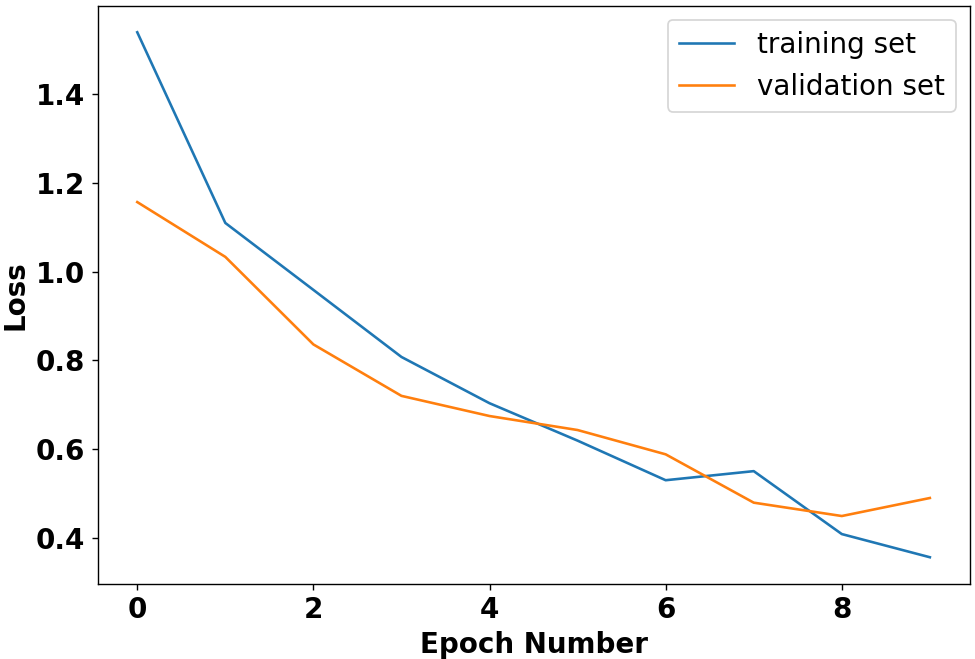
\includegraphics[width=\textwidth]{images/activity-initial-test-loss.png}
        \caption{Loss plot}
        \label{fig:activity-initial-test-loss}
    \end{subfigure}
    \qquad
    \begin{subfigure}{0.4\textwidth}
        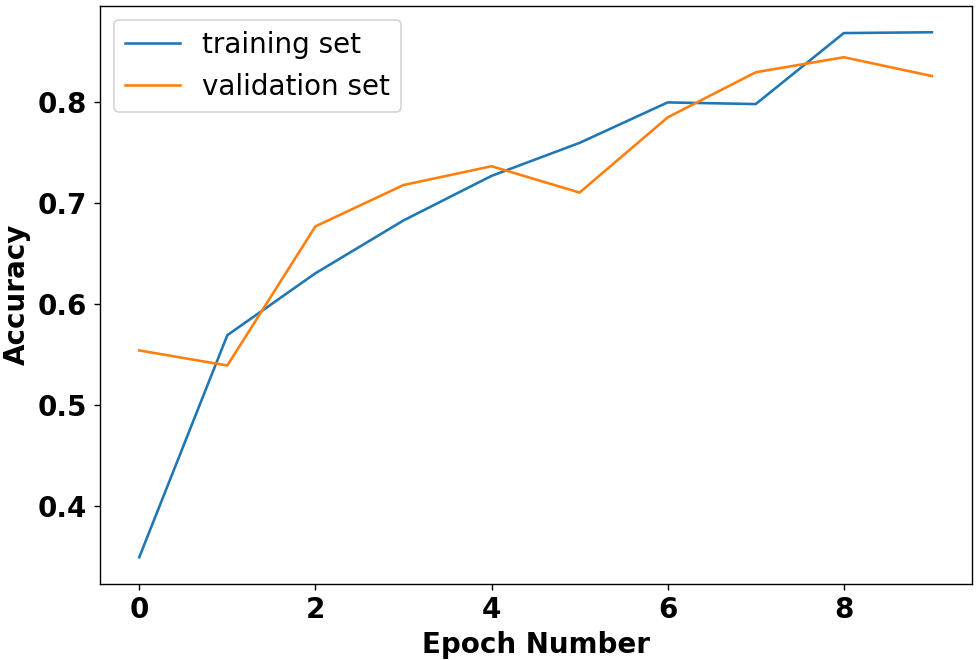
\includegraphics[width=\textwidth]{images/activity-initial-test-accuracy.png}
        \caption{Accuracy plot}
        \label{fig:activity-initial-test-accuracy}
    \end{subfigure}
  \caption{\subref{fig:activity-initial-test-loss} shows the loss value of training and validation set over training epochs. Subsequently, \subref{fig:activity-initial-test-accuracy} shows that of accuracy. The plots shows that the learning have not converge yet and there are more rooms for improvement.}
  \label{fig:acitivity-initial-loss-and-accuracy-plots}
\end{figure}

Upon evaluating the model with an unseen test set, it achieved an accuracy of 68.46\%, with precision, recall, and F1-score values of 0.73, 0.76, and 0.70, respectively. Figure \ref{fig:acitivity-initial-prediction-plots-and-confusion-matrix} presents some prediction outcomes and the confusion matrix. A comparison with the training phase results reveals a possibility of overfitting, as indicated by the model's suboptimal generalization to new data.
\begin{figure}[h]
   \centering
   \begin{subfigure}{0.4\textwidth}
        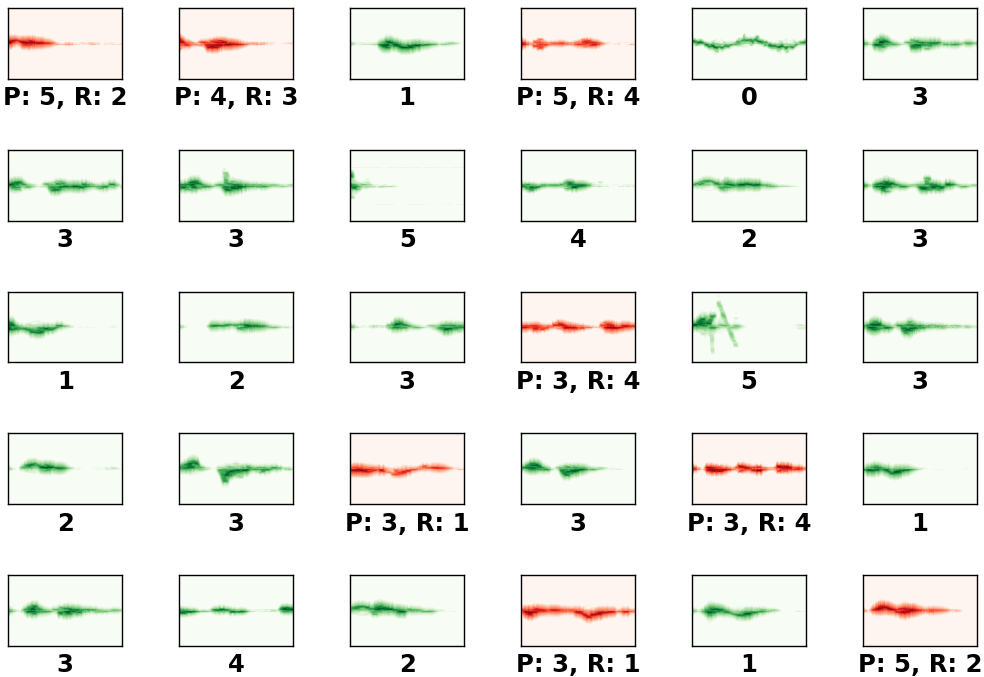
\includegraphics[width=\textwidth]{images/activity-initial-test-prediction-plots.png}
        \caption{Prediction plots}
        \label{fig:activity-initial-test-prediction-plots}
    \end{subfigure}
    \qquad
    \begin{subfigure}{0.4\textwidth}
        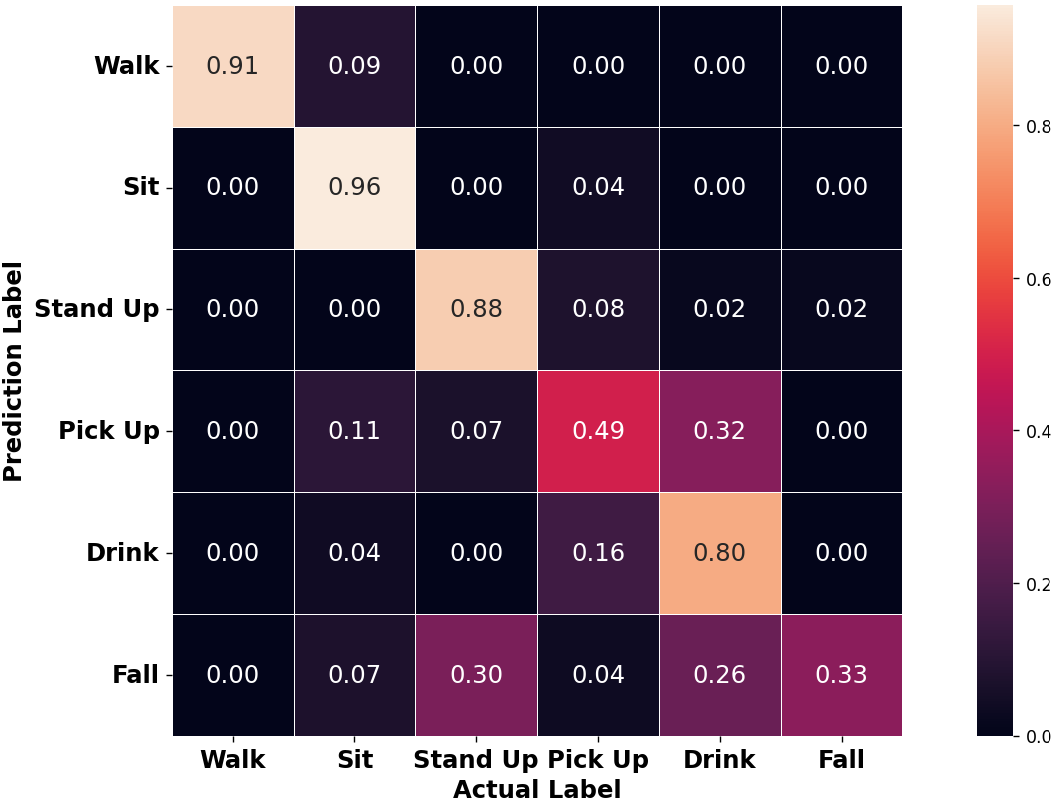
\includegraphics[width=\textwidth]{images/activity-initial-test-confusion-matrix.png}
        \caption{Confusion matrix}
        \label{fig:activity-initial-test-confusion-matrix}
    \end{subfigure}
  \caption{The figures shows the prediction performance of the baseline CNN model on the test set. \subref{fig:activity-initial-test-prediction-plots} displays some of the sample predictions. The green-colored graph represents correct predictions, while red-colored graph represents wrong ones (P stands for prediction label and R for real/actual label).\subref{fig:activity-initial-test-confusion-matrix} shows the confusion matrix of the predictions.}
  \label{fig:acitivity-initial-prediction-plots-and-confusion-matrix}
\end{figure}

\newpage

\subsection{Hyperparameter Tuning}
In our study, we experimented with both the initial and the refined data splitting strategies. Given that the results from both approaches were quite similar, and for clarity, we have chosen to present the hyperparameter tuning and ablation study outcomes based on the initial data splitting strategy applied to the full radar dataset of 106 participants.

Hyperparameter tuning involves exploring the hyperparameter space to identify optimal parameter values for model training and to understand their impact on performance. As detailed in Table \ref{tab:activity-hyperparameter-tuning} in the appendix, we adjusted parameters such as batch size, epochs, and learning rate during the tuning process. The table findings indicate that a batch size of 8, an epoch count of 13, and a learning rate of 0.0005 yielded the best results for the baseline CNN model. Next, we will delve into the ablation study to adjust the CNN layers.

\subsection{Ablation Study}
An ablation study investigates the model's performance by systematically adding or removing CNN layers. This process helps to discern the contribution of each layer and identify the optimal CNN layer configurations for the best performance outcome. The results of the ablation study for activity classification are presented in Table \ref{tab:activity-ablation-study} in the appendix. This table outlines various adjustments to the CNN layers, including the addition of extra convolution layers with varying numbers of filters and the incorporation of dropout layers with different rates. According to the findings, the most effective CNN configuration is identified as configuration number 4. This setup includes three additional layers: a convolution layer with 128 filters, a dropout layer with a rate of 0.2, and another convolution layer with 256 filters.

\subsection{Optimal CNN Model Configuration}
Based on the findings from the ablation study presented in Table \ref{tab:activity-ablation-study}, we have identified configuration number 3 as our optimal CNN model configuration. Table \ref{tab:activity-final-CNN-configuration} details the finalized CNN layer configurations along with their specific parameter values. We have fine-tuned the learning rate to 0.0005, set the training duration to 13 epochs, and chosen a batch size of 8. For optimization, we utilized the Adam optimizer, paired with Categorical Cross-entropy as the loss function and accuracy as the metric for evaluation.

\begin{table}[ht]
    \centering
    \begin{tabular}{ccccc}
        \toprule
        \textbf{Layer} & \textbf{Filter No.} & \textbf{Kernel Size} & \textbf{Activation Type} & \textbf{Rate (0-1)} \\
        \midrule
        \midrule
        Convolution & 32  & 3x3 & ReLu & - \\
        Max Pooling & - & 2x2 & ReLu & - \\
        Convolution & 64 & 3x3 & ReLu & - \\
        Max Pooling & - & 2x2 & ReLu & - \\
        Convolution & 128 & 3x3 & ReLu & - \\
        Max Pooling & - & 2x2 & ReLu & - \\
        Convolution & 256 & 3x3 & ReLu & - \\
        Max Pooling & - & 2x2 & ReLu & - \\
        Flatten & - & - & - & - \\
        Dense & 64 & - & ReLu & - \\
        Dropout & - & - & - & 0.2 \\
        Dense & 6 & - & Softmax  & - \\
        \bottomrule
    \end{tabular}
    \caption{Optimal CNN model configuration of the activity classification task.}
    \label{tab:activity-final-CNN-configuration}
\end{table}

\subsection{Optimal Performance Evaluation}
As demonstrated by the results of configuration number 4 in Table \ref{tab:activity-ablation-study}, the highest accuracy and F1-score achieved were 90.00\% and 0.91, respectively. Precision and recall were recorded at 0.92 and 0.91, respectively, from testing the model with the unseen test set. When comparing this optimal performance with the baseline results shown in \ref{activity_baseline_performance_result}, we observe substantial improvements across all classification metrics: accuracy, precision, recall, and F1-score, increased by 21.54\%, 0.19, 0.15, and 0.21, respectively. The enhancements between the baseline and optimal CNN configurations are illustrated in the bar charts of Figure \ref{fig:activity-configuration-comparison}.

\begin{figure}[h]
   \centering
   \begin{subfigure}{0.4\textwidth}
        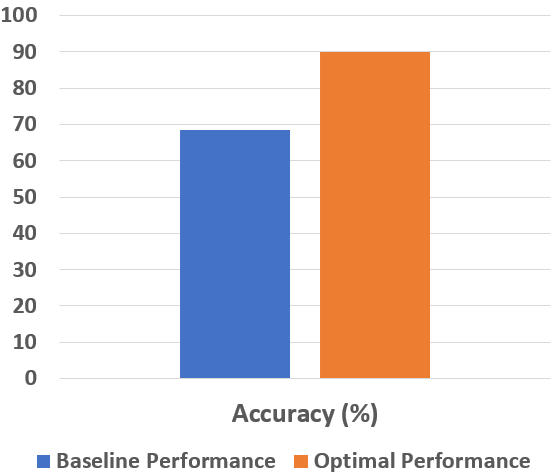
\includegraphics[width=\textwidth]{images/activity-configuration-comparison-barchart1.png}
        \caption{Accuracy (\%)}
        \label{fig:activity-configuration-comparison-barchart1}
    \end{subfigure}
    \qquad
    \begin{subfigure}{0.4\textwidth}
        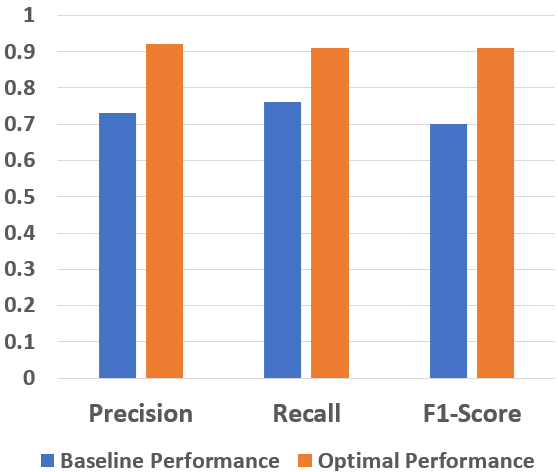
\includegraphics[width=\textwidth]{images/activity-configuration-comparison-barchart2.png}
        \caption{Precision, Recall, F1-Score}
        \label{fig:activity-configuration-comparison-barchart2}
    \end{subfigure}
  \caption{The bar charts display the improvements in the performance between the baseline CNN model and optimal CNN model of the activity classification task.}
  \label{fig:activity-configuration-comparison}
\end{figure}

The bar charts shown in Figure \ref{fig:activity-configuration-comparison} highlight the improvement in the model’s capacity to classify activities using radar data. The optimal results showcase satisfying accuracy across all classification metrics. This suggests that the model maintains a balanced performance between precision and recall, emphasizing the model’s robustness. Overall, the model demonstrates strong predictive capability and reliability across the evaluation criteria. 

Figure \ref{fig:acitivity-final-prediction-plots-and-confusion-matrix} displays prediction plots and a confusion matrix for the optimal CNN model’s performance on the unseen test set. This analysis allows us to evaluate how effectively the model distinguishes between different activities. It is evident that activities such as walking, sitting, standing up, and falling frontwards are easily discernible, as the majority were predicted correctly. However, the model encounters slight difficulty differentiating between "picking up an object" and "drinking from a glass". We can compare the optimal confusion matrix result to the baseline from Figure \ref{fig:acitivity-initial-prediction-plots-and-confusion-matrix}.

\begin{figure}[h]
    \centering
    \begin{subfigure}{0.4\textwidth}
        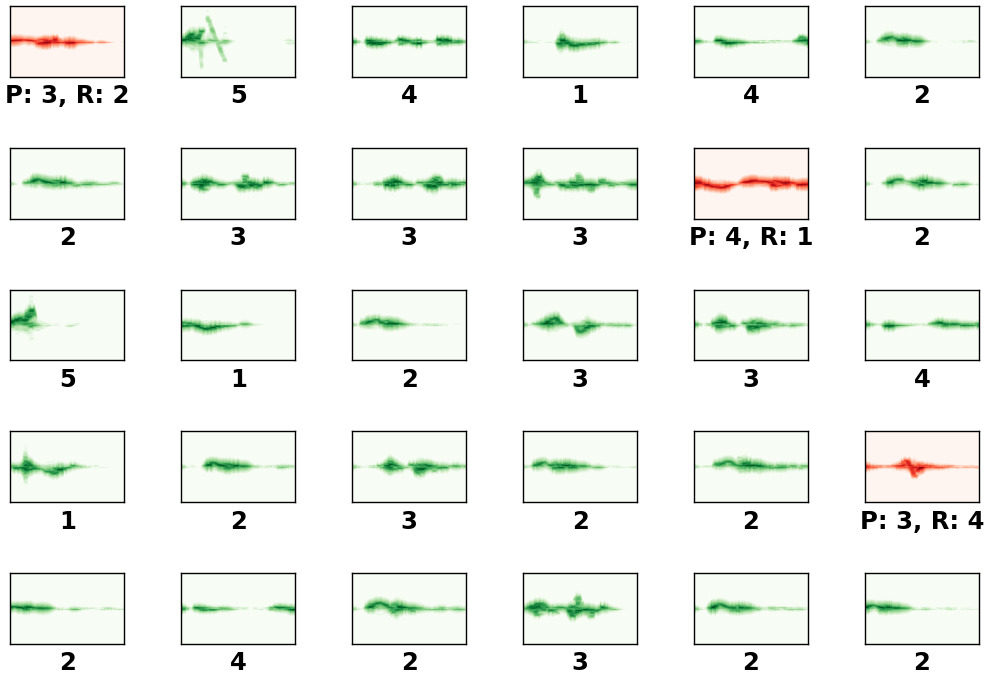
\includegraphics[width=\textwidth]{images/activity-final-test-prediction-plots.png}
        \caption{Prediction plots}
        \label{fig:activity-final-test-prediction-plots}
    \end{subfigure}
    \qquad
    \begin{subfigure}{0.4\textwidth}
        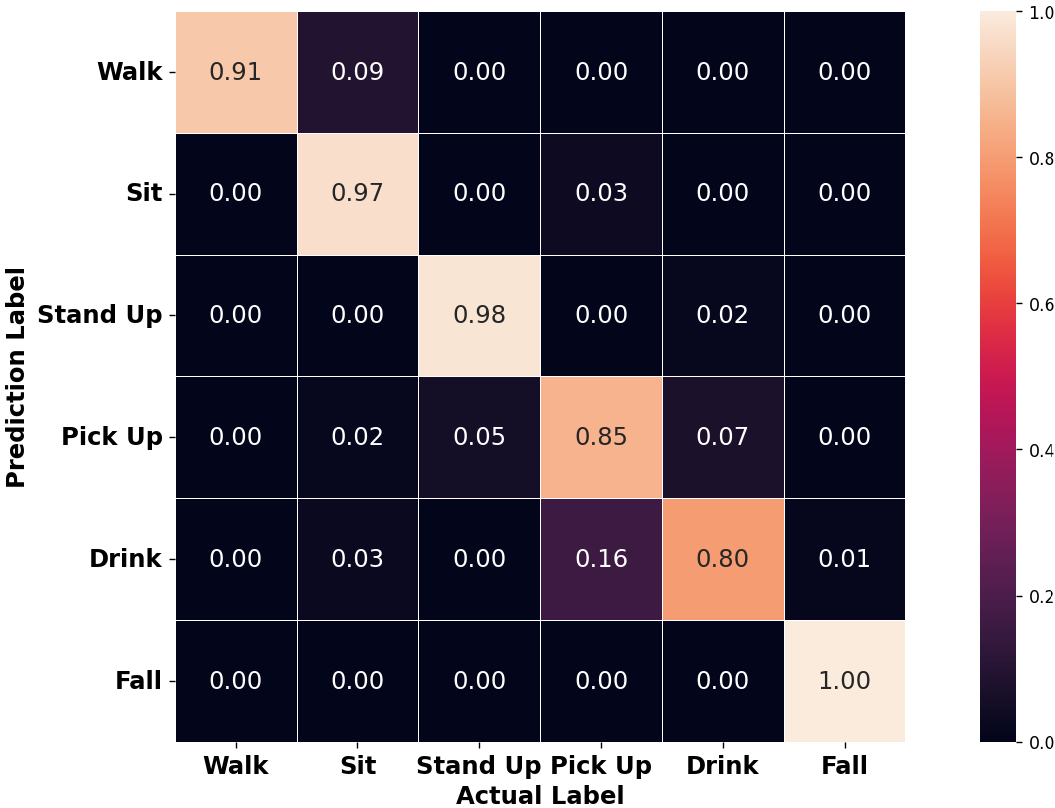
\includegraphics[width=\textwidth]{images/activity-final-test-confusion-matrix.png}
        \caption{Confusion matrix}
        \label{fig:activity-final-test-confusion-matrix}
    \end{subfigure}
    \caption{This figure shows the prediction plots \subref{fig:activity-final-test-prediction-plots} and confusion matrix \subref{fig:activity-final-test-confusion-matrix} of the optimal CNN model on the test set. The green-colored graph represents correct predictions, while red-colored graph represents wrong ones (P stands for prediction label and R for real/actual label).}
    \label{fig:acitivity-final-prediction-plots-and-confusion-matrix}
\end{figure}

\subsection{Data Augmentation Evaluation}
The performance results presented earlier were based on model training without incorporating data augmentations. This section evaluates the impact of employing data augmentation methods as described in Section \ref{data_augmentation}. To maintain fairness and consistency in future evaluations of data augmentation for participant identification and multi-task sections, we have applied the refined data splitting strategy to the 30-participant dataset. Table \ref{tab:activity-classification-data-augmentations-evaluation}, in the appendix, outlines the results of this data augmentation evaluation. For each method, the model underwent training and evaluation five times to determine the average prediction performance. The results, including accuracy and F1-score, are presented in the table in an $Accuracy | F1-score$ format. According to the table, mixup data augmentation yielded the best results, achieving an average accuracy of 92.79\% and an average F1-score of 0.92. Consequently, the best performance we obtained is an accuracy of 96.72\% and a F1-score of 0.97. However, the average differences between the outcomes of each data augmentation method were relatively minor.

\section{Participant Identification Evaluation}
The number of potential participant labels depends on the dataset utilized. For instance, a dataset with 30 participants requires a one-hot encoding array of size 30. In this section, we present the result based on using the 30-participant dataset. To be candid, configuring the CNN model to deliver satisfactory participant identification performance proved to be a significant challenge.  Achieving desirable performance outcomes without employing data augmentation techniques was nearly impossible. Therefore, all experiments detailed below utilize the axis-flipping data augmentation method. Subsequently, it will be demonstrated that this data augmentation method yields the best results.

\subsection{Baseline Performance Result}
Similar to the activity classification task, we establish a baseline result as our evaluation starting point. Table \ref{tab:participant-initial-CNN-configuration} in the appendix displays the baseline CNN model configuration, with an initial learning rate set at 0.001, 10 epochs, and a batch size of 64.

The baseline performance is shown to be significantly below expectations. Figure \ref{fig:participant-initial-loss-and-accuracy-plots} shows the training and validation losses and accuracies for each epoch during the training process. The analysis suggests that the model has not yet converged, highlighting a significant opportunity for hyperparameter tuning and further ablation studies.

\begin{figure}[h]
   \centering
   \begin{subfigure}{0.4\textwidth}
        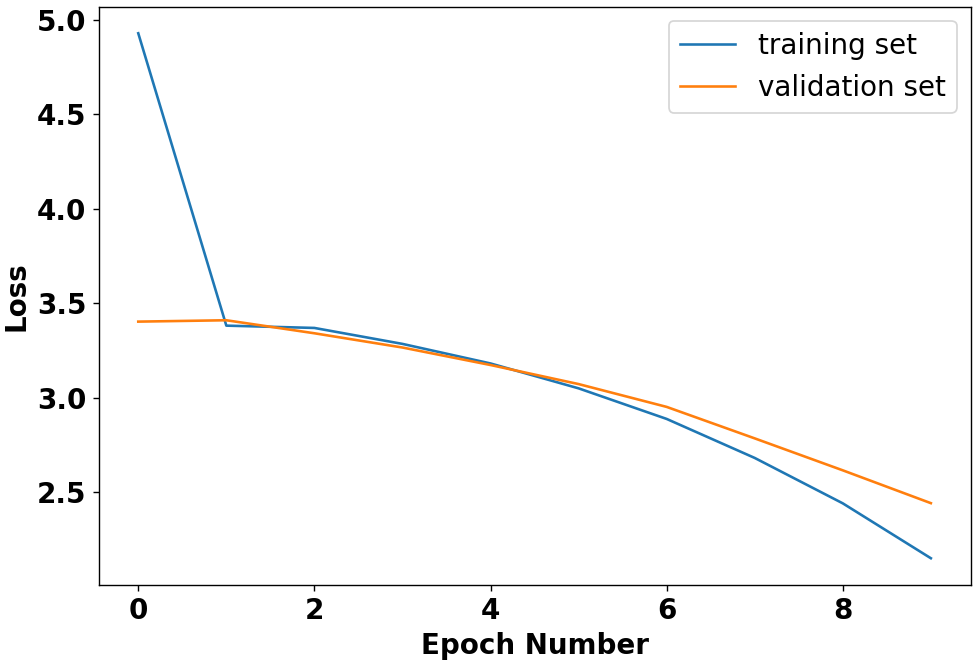
\includegraphics[width=\textwidth]{images/participant-initial-test-loss.png}
        \caption{Loss plot}
        \label{fig:participant-initial-test-loss}
    \end{subfigure}
    \qquad
    \begin{subfigure}{0.4\textwidth}
        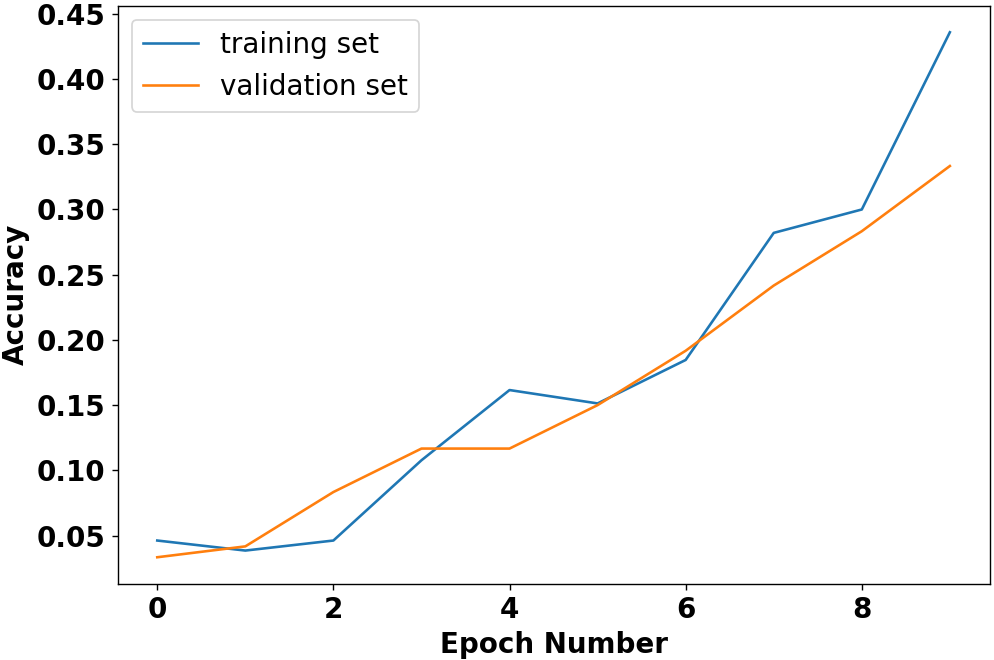
\includegraphics[width=\textwidth]{images/participant-initial-test-accuracy.png}
        \caption{Accuracy plot}
        \label{fig:participant-initial-test-accuracy}
    \end{subfigure}
  \caption{\subref{fig:participant-initial-test-loss} shows the baseline loss value of the training and validation set over epochs. Subsequently, \subref{fig:participant-initial-test-accuracy} shows that of accuracy.}
  \label{fig:participant-initial-loss-and-accuracy-plots}
\end{figure}

Figure \ref{fig:participant-initial-prediction-plots-and-confusion-matrix} presents the prediction performance of the baseline CNN model on the unseen test set. The model achieved a prediction accuracy of 36.67\%, with precision, recall, and F1-score values of 0.26, 0.37, and 0.29, respectively. These results underscore the initial CNN model's poor performance and the necessity for substantial adjustments to enhance its effectiveness.
\begin{figure}[h]
   \centering
   \begin{subfigure}{0.4\textwidth}
        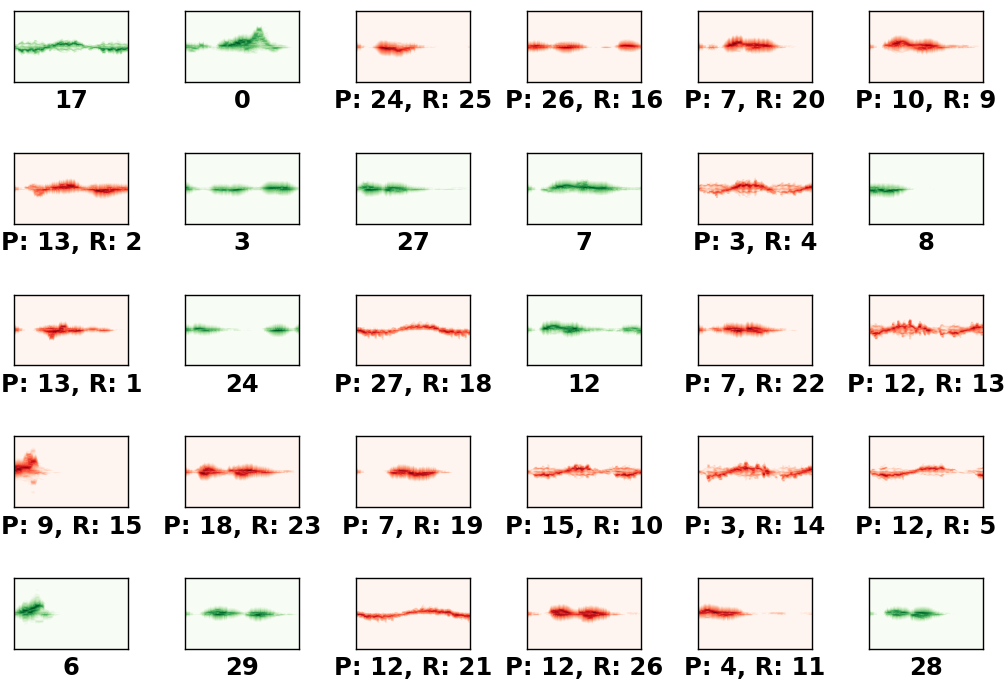
\includegraphics[width=\textwidth]{images/participant-initial-test-prediction-plots.png}
        \caption{Prediction plots}
        \label{fig:participant-initial-test-prediction-plots}
    \end{subfigure}
    \qquad
    \begin{subfigure}{0.4\textwidth}
        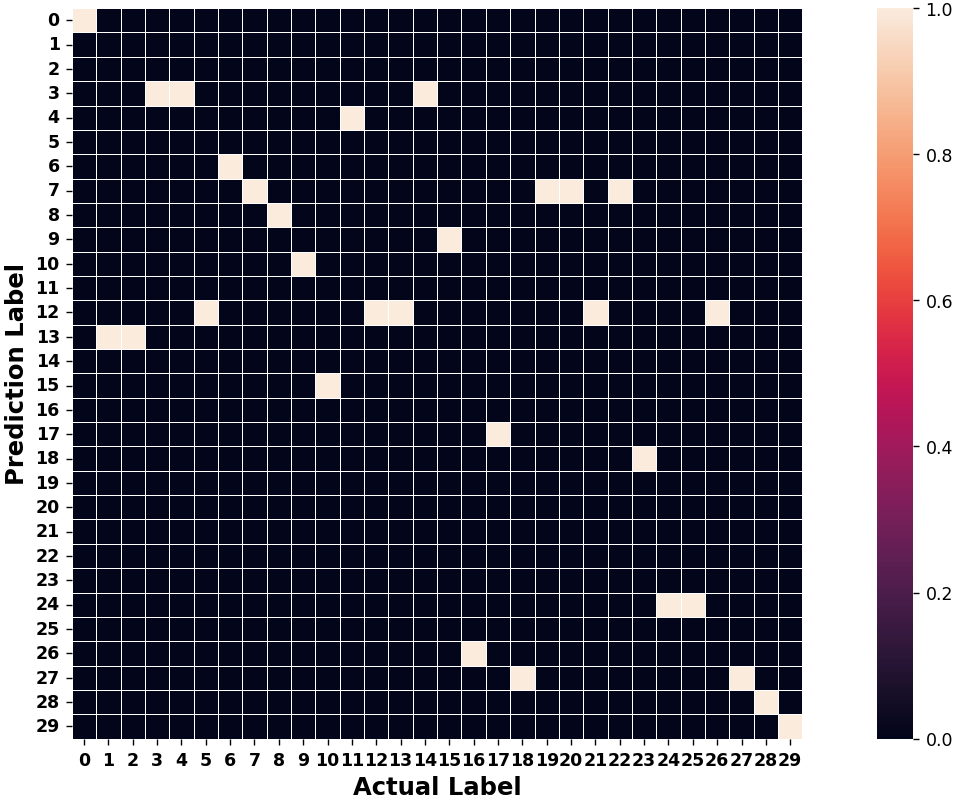
\includegraphics[width=\textwidth]{images/participant-initial-test-confusion-matrix.png}
        \caption{Confusion matrix}
        \label{fig:participant-initial-test-confusion-matrix}
    \end{subfigure}
  \caption{The figures shows the prediction performance of the baseline CNN model on the test set. \subref{fig:participant-initial-test-prediction-plots} displays some of the sample predictions. The green-colored graph represents correct predictions, while red-colored graph represents wrong ones, where P stands for prediction label and R for real/actual label. \subref{fig:participant-initial-test-confusion-matrix} shows the confusion matrix of the predictions.}
  \label{fig:participant-initial-prediction-plots-and-confusion-matrix}
\end{figure}

\subsection{Hyperparameter Tuning}
Unlike the activity classification task, participant identification presents a more complex challenge, necessitating extensive experimentation to navigate the hyperparameter space effectively. Some of the outcomes of the hyperparameter tuning experiment are detailed in Table \ref{tab:participant-hyperparameter-tuning} in the appendix. This table includes adjustments to batch size, learning rate, and the number of epochs. It is important to note that the results regarding epoch number adjustments in the table reflect performance outcomes after completing the ablation study. Adjusting each hyperparameter individually did not lead to performance improvements, highlighting the nuanced approach required for optimizing participant identification models.

\subsection{Ablation Study}
The ablation study, detailed in Table \ref{tab:participant-ablation-study} in the appendix, showcases some of the experimented model configurations and their outcomes. These configurations involve the addition of layers such as convolution and dropout layers. The table reveals that configuration number 5 yields the best performance among all tested setups, achieving an accuracy of 76.67\% and an F1-score of 0.71. Given the promising result, we proceeded to further refine this model configuration through additional hyperparameter tuning, as shown in Table \ref{tab:participant-hyperparameter-tuning}, aiming to identify the optimal CNN configuration and hyperparameters.

\subsection{Optimal CNN Model Configuration}
The optimal performance obtained for participant identification can be found in the hyperparameter tuning table \ref{tab:participant-hyperparameter-tuning}. The performance result is highlighted within the "Tuning Epoch Number" subsection. Table \ref{tab:participant-final-CNN-configuration} outlines the finalized CNN layer configurations from our experiment. The learning rate has been fine-tuned to 0.00015, with the model trained over 60 epochs, and a batch size set to 32. For optimization, we chose the Adam optimizer, using categorical crossentropy as the loss function and accuracy as the metric for evaluation.

\begin{table}[h]
    \centering
    \begin{tabular}{ccccc}
        \toprule
        \textbf{Layer} & \textbf{Filter No.} & \textbf{Kernel Size} & \textbf{Activation Type} & \textbf{Rate (0-1)} \\
        \midrule
        \midrule
        Convolution & 32  & 3x3 & ReLu & - \\
        Max Pooling & - & 2x2 & ReLu & - \\
        Convolution & 64 & 3x3 & ReLu & - \\
        Max Pooling & - & 2x2 & ReLu & - \\
        Convolution & 128 & 3x3 & ReLu & - \\
        Max Pooling & - & 2x2 & ReLu & - \\
        Convolution & 256 & 3x3 & ReLu & - \\
        Max Pooling & - & 2x2 & ReLu & - \\
        Flatten & - & - & - & - \\
        Dropout & - & - & - & 0.25 \\
        Dense & 128 & - & ReLu & - \\
        Dropout & - & - & - & 0.3 \\
        Dense & 64 & - & ReLu & - \\
        Dropout & - & - & - & 0.5 \\
        Dense & 30 & - & Softmax & - \\
        \bottomrule
    \end{tabular}
    \caption{Optimal CNN configuration of participant identification task.}
    \label{tab:participant-final-CNN-configuration}
\end{table}

\subsection{Optimal Performance Evaluation}
The optimal performance achieved includes an accuracy of 86.67\%, with precision at 0.80, recall at 0.87, and an F1-score of 0.82. Comparing this to the baseline performance reveals significant improvements across all metrics.  Specifically, accuracy, precision, recall, and F1-score have increased by 50.00\%, 0.54, 0.50, and 0.53, respectively. The enhancement in performance from the baseline to the optimal CNN configuration is depicted in Figure \ref{fig:participant-configuration-comparison}.

\begin{figure}[h]
    \centering
    \begin{subfigure}{0.4\textwidth}
        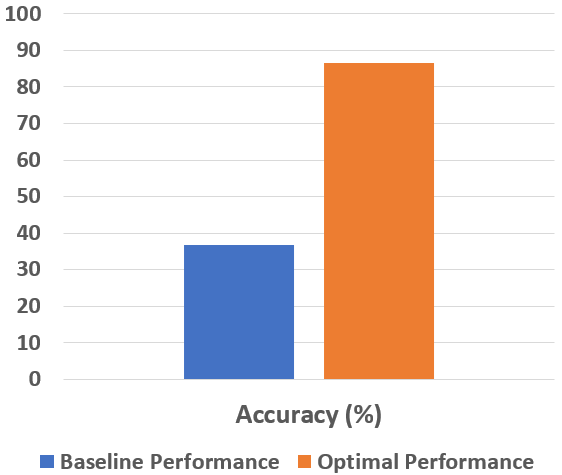
\includegraphics[width=\textwidth]{images/participant-configuration-comparison-barchart1.png}
        \caption{Accuracy (\%)}
        \label{fig:participant-configuration-comparison-barchart1}
    \end{subfigure}
    \qquad
    \begin{subfigure}{0.4\textwidth}
        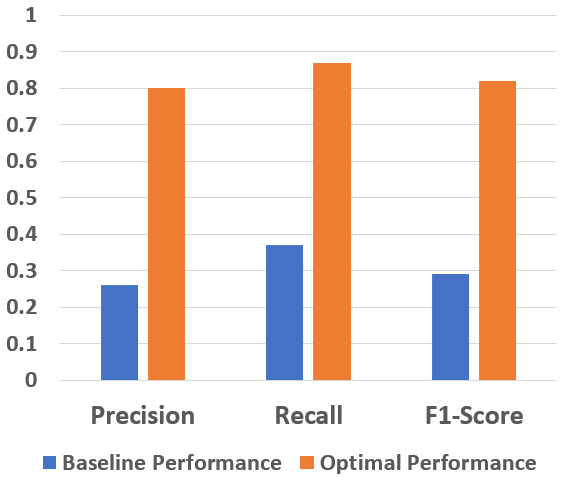
\includegraphics[width=\textwidth]{images/participant-configuration-comparison-barchart2.png}
        \caption{Precision, Recall, F1-Score}
        \label{fig:participant-configuration-comparison-barchart2}
    \end{subfigure}
    \caption{The bar charts display the improvements in performance between baseline and optimal performance of participant identification task.}
    \label{fig:participant-configuration-comparison}
\end{figure}

Based on Figure \ref{fig:participant-configuration-comparison}, it is noticeable that the precision metric has shown the most significant increase, albeit by a slim margin over the other classification metrics. Furthermore, the recall metric emerges as the highest classification metric, indicating that the model is particularly effective at identifying true positive instances—participants within the dataset—while minimizing false negatives. This characteristic is especially beneficial for security-related applications, where accurately recognizing all authorized individuals is crucial to prevent unauthorized access. Additionally, with a precision of 0.80, the model demonstrates a low rate of false positives, suggesting a high likelihood of correct participant label predictions.

Figure \ref{fig:participant-final-prediction-plots-and-confusion-matrix} presents the prediction plots and the confusion matrix for the optimal CNN model's performance on the unseen test set. The confusion matrix reveals a pronounced diagonal line, indicating that the most of the participant labels were correctly predicted. To observe the contrast, we can compare it with the baseline confusion matrix in Figure \ref{fig:participant-initial-prediction-plots-and-confusion-matrix}.

\begin{figure}[h]
    \centering
    \begin{subfigure}{0.4\textwidth}
        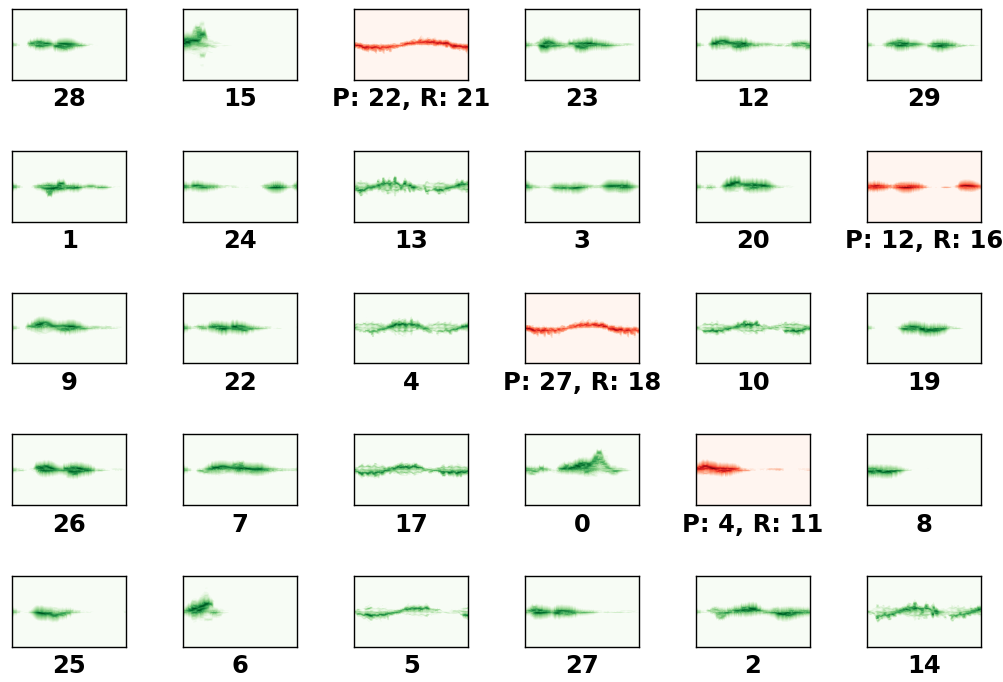
\includegraphics[width=\textwidth]{images/participant-final-test-prediction-plots.png}
        \caption{Prediction plots}
        \label{fig:participant-final-test-prediction-plots}
    \end{subfigure}
    \qquad
    \begin{subfigure}{0.4\textwidth}
        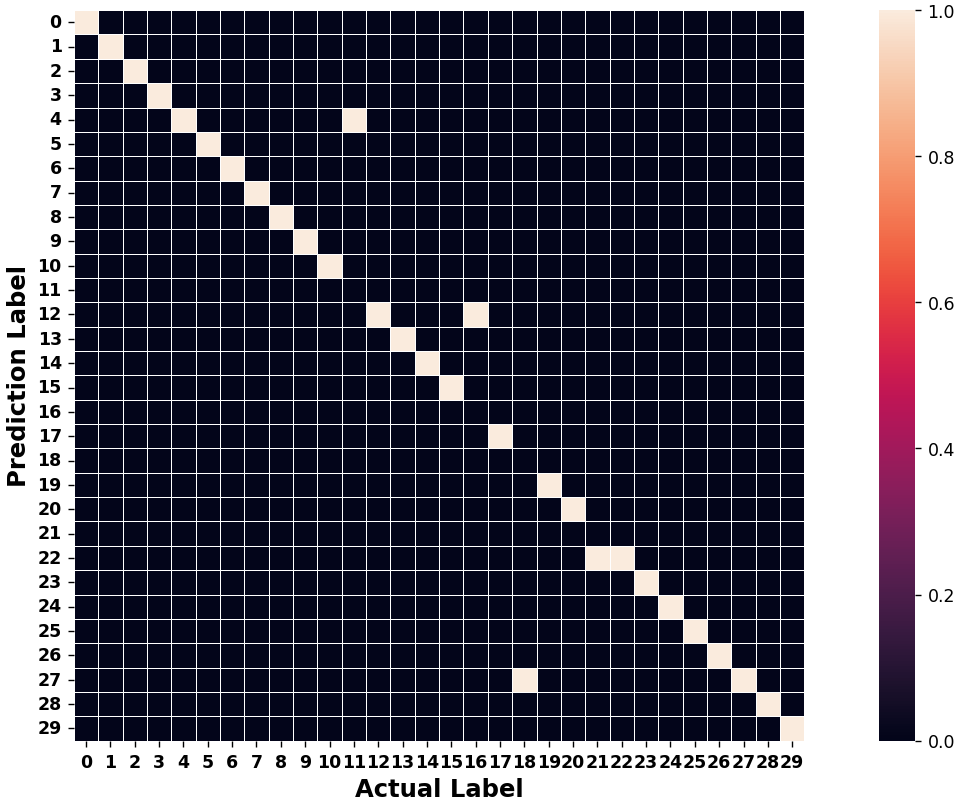
\includegraphics[width=\textwidth]{images/participant-final-test-confusion-matrix.png}
        \caption{Confusion matrix}
        \label{fig:participant-final-test-confusion-matrix}
    \end{subfigure}
    \caption{The figures shows the prediction performance of the optimal CNN model on the test set. \subref{fig:participant-final-test-prediction-plots} displays some of the sample predictions. \subref{fig:participant-final-test-confusion-matrix} shows the confusion matrix of the predictions.}
    \label{fig:participant-final-prediction-plots-and-confusion-matrix}
\end{figure}

\subsection{Data Augmentation Evaluation}
The experimental results shown above are based on utilizing axis-flipping data augmentation, which proved to be the most effective. This section aims to underscore this point by comparing the outcomes derived from other data augmentation techniques. Table \ref{tab:participant-recognition-data-augmentations-evaluation}, in the appendix, presents the experimental results for each data augmentation approach. Mirroring the evaluation process used in the activity classification task, we trained the model five times for each method and calculated the average performance. Each training outcome was documented in the format of $Accuracy | F1-score$. The table confirms that the axis-flipping method indeed yields the best results, with an average accuracy of 82.67\% and an average F1-score of 0.78. It is evident that the results obtained from this method are comparatively better than those of mixup augmentation and no augmentation at all. Consequently, the best performance obtained is an accuracy of 86.67\% and F1-score of 0.82.

\subsection{Participant Identification by Activity}
As a supplementary experiment, we evaluated the ability to identify participants based on individual activities. We further categorized the 61-participant dataset based on the six activities. The detail of the activity-categorized samples can be viewed in Table \ref{tab:participant-identification-by-activity} in the appendix. Analyzing performance in this manner can provide insights into the unique behavioral patterns of participants associated with each activity. Essentially, if the model demonstrates ease in classifying participants by an activity, it implies that participants exhibit distinct and distinguishable movement patterns for that activity.

From our experiments, we discovered that the walking activity posed the greatest challenge for participant identification, with an accuracy rate of only 37.70\%. In contrast, the activities such as "picking up an object" and "drinking from a glass" proved to be the easiest for the model to classify, achieving accuracy rates of approximately 65.57\% and 59.02\%, respectively. These results suggest that the behavioral movements of the two activities present more unique identifiable patterns compared to other activities. While these results may seem suboptimal, they are still considered reasonable and promising given the constraints of limited data resources. We believe that with a larger training and validation dataset, the model's identification performance could be significantly improved for all activities.

\section{Multi-task Model Evaluation}
For this evaluation, we applied the refined data splitting strategy to the 30-participant dataset. Our multi-task model features a shared-bottom architecture, where the CNN layers in the feature extraction phase are common across tasks, diverging only for their respective classification phases. The structure of the model is illustrated in Figure \ref{fig:multi-task-model} in the design chapter. As with the participant identification evaluation, all experiments conducted for this section utilized the axis-flipping data augmentation technique.

\subsection{Baseline Performance Result}
Table \ref{tab:multitask-initial-CNN-configuration} outlines the baseline CNN configuration for our multi-task model, reflecting the final CNN configurations for each specific task. In this setup, the Dense2 layer is responsible for generating one-hot encodings for activity classification predictions, whereas Dense5 layer does the same for participant recognition. The model begins with a learning rate of 0.001, runs for 15 epochs, and has a batch size of 32. Moreover, in multi-task settings, given that different tasks can vary in complexity or importance, it is essential to adjust initial loss weights to facilitate effective learning. Beginning with a weight of 1.0 for the activity task and 8.0 for the participant task proves to be a suitable starting point. Starting with equal weights of 1.0 for both tasks would lead to the activity task's loss dominating over that of the participant task.

Figure \ref{fig:multitask-initial-loss-and-accuracy-plots} displays the loss and accuracy values recorded during training and validation phases of the model. The loss lines for the training and validation sets are depicted in red and pink, respectively, showing a trend towards convergence. Similarly, the accuracy lines for the training and validation sets, represented in blue and cyan, also follow a similar pattern. However, the lack of complete convergence in these lines indicates that there is room for further enhancements in the model's performance.

\begin{figure}[h]
   \centering
   \begin{subfigure}{0.47\textwidth}
        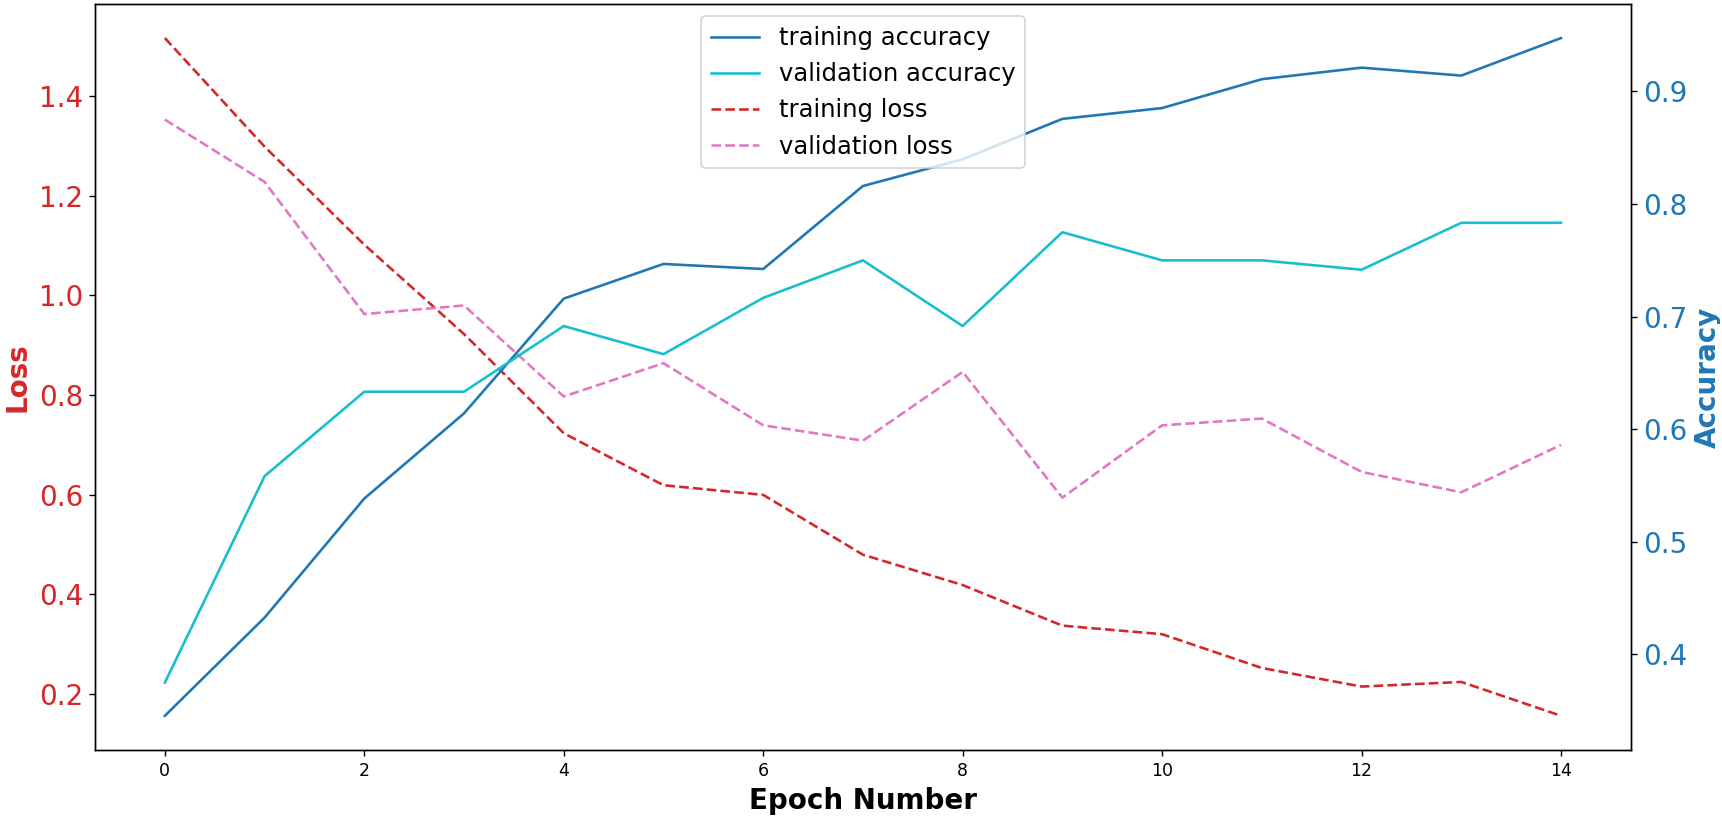
\includegraphics[width=\textwidth]{images/multitask-activity-initial-test.png}
        \caption{Activity loss and accuracy plot during training}
        \label{fig:multitask-activity-initial-test}
    \end{subfigure}
    \qquad
    \begin{subfigure}{0.47\textwidth}
        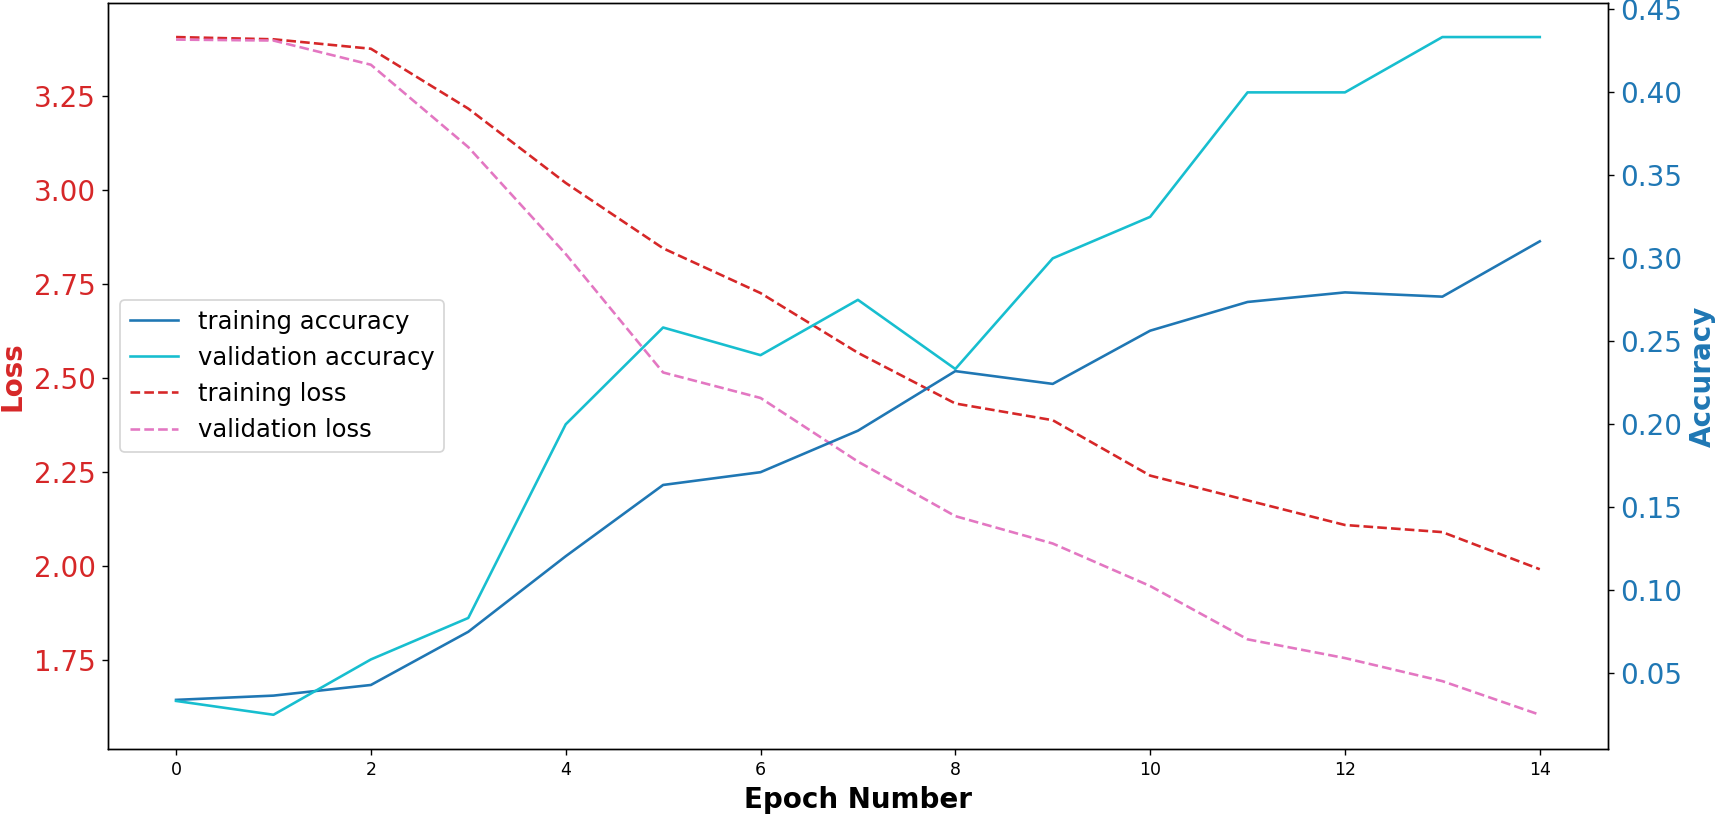
\includegraphics[width=\textwidth]{images/multitask-participant-initial-test.png}
        \caption{Participant loss and accuracy plot during training}
        \label{fig:multitask-participant-initial-test}
    \end{subfigure}
  \caption{\subref{fig:multitask-activity-initial-test} shows the activity loss and accuracy values of training and validation set over number of epochs. Subsequently, \subref{fig:participant-initial-test-accuracy} shows that of participant's. The loss plotted lines are shown in red (training set) and pink (validation set) and the accuracy plotted lines are shown in blue (training set) and cyan (validation set).}
  \label{fig:multitask-initial-loss-and-accuracy-plots}
\end{figure}

The baseline results depicted in Figure \ref{fig:multitask-initial-confusion-matrices} reveal that the activity classification task surpasses the participant recognition task in terms of performance. The CNN multi-task model shows satisfactory results in classifying activities, with an accuracy of 76.67\%, and commendable precision (0.75), recall (0.81), and F1-score (0.76). Conversely, the accuracy for participant recognition stands at 56.67\%, indicating potential areas for enhancement, as evidenced by lower precision (0.46), recall (0.57), and F1-score (0.49). These outcomes highlight the model's proficiency in identifying activities while underscoring the need for improvement in participant recognition. Future efforts could aim to refine the performance of both tasks, aiming for a more balanced result.

\begin{figure}[h]
   \centering
   \begin{subfigure}{0.49\textwidth}
        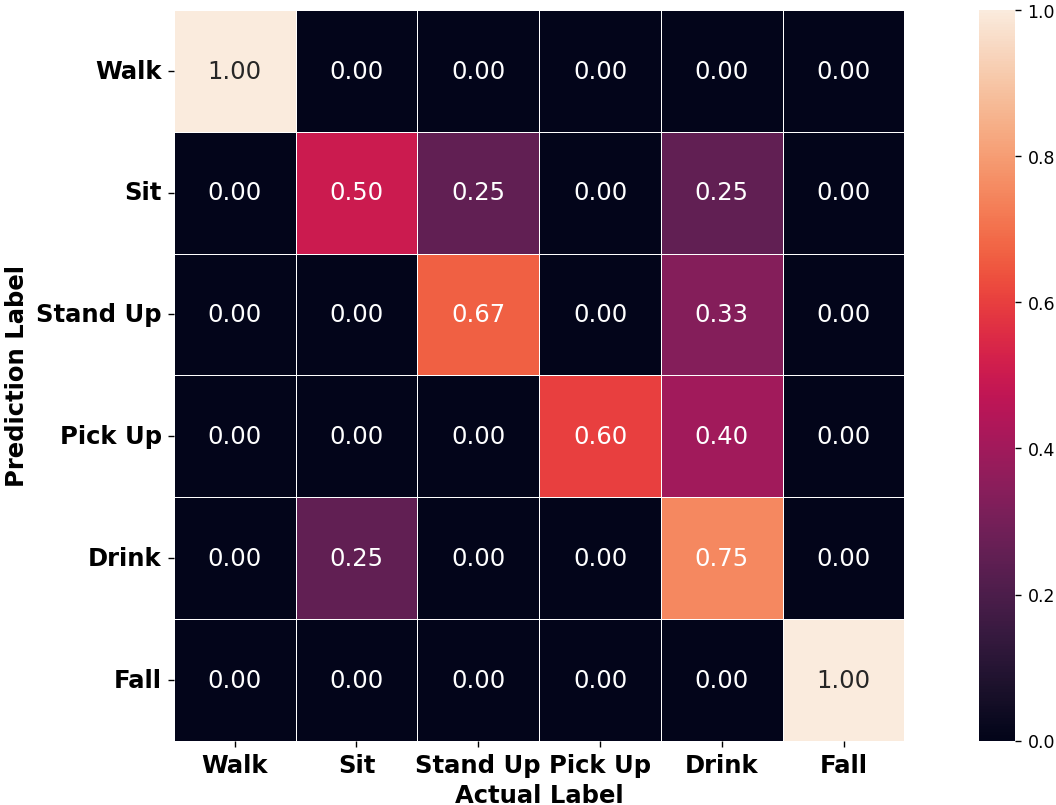
\includegraphics[width=\textwidth]{images/multitask-activity-initial-test-confusion-matrix.png}
        \caption{Activity confusion matrix}
        \label{fig:multitask-activity-initial-test-confusion-matrix}
    \end{subfigure}
    \qquad
    \begin{subfigure}{0.45\textwidth}
        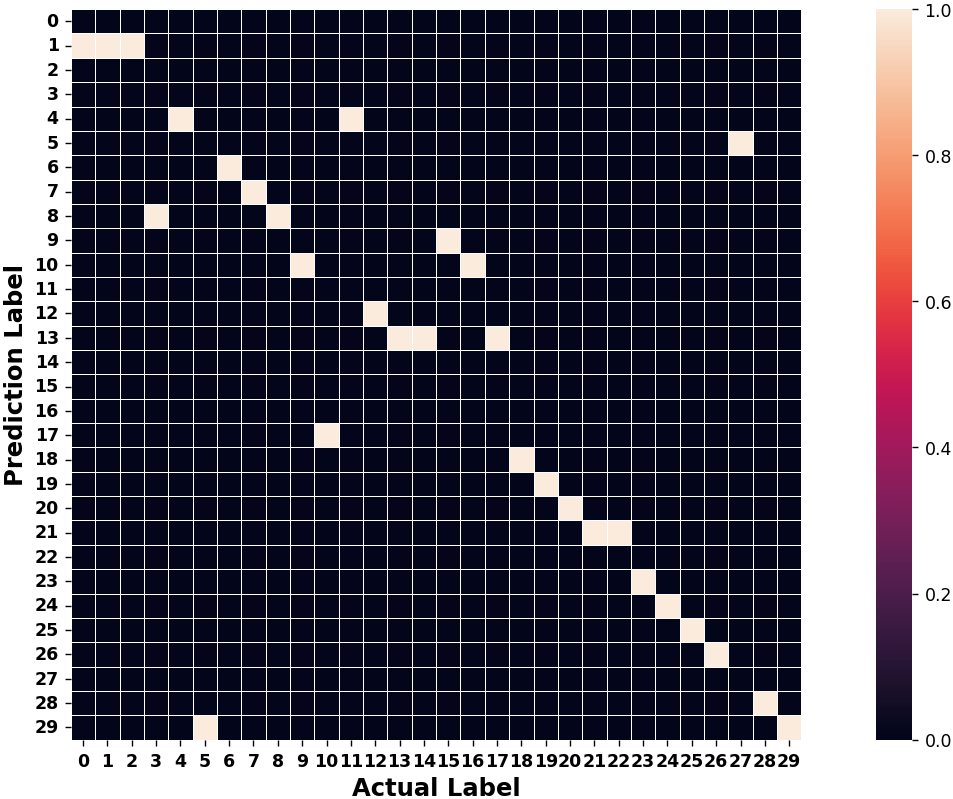
\includegraphics[width=\textwidth]{images/multitask-participant-initial-test-confusion-matrix.png}
        \caption{Participant confusion matrix}
        \label{fig:multitask-participant-initial-test-confusion-matrix}
    \end{subfigure}
  \caption{The figures shows the prediction performance of the baseline multi-task model on the test set. \subref{fig:multitask-activity-initial-test-confusion-matrix} displays the confusion matrix of activity classification task. \subref{fig:multitask-participant-initial-test-confusion-matrix} shows the confusion matrix of participant recognition task.}
  \label{fig:multitask-initial-confusion-matrices}
\end{figure}

\subsection{Hyperparameter Tuning}
Similar to the approach taken in previous evaluation sections, we fine-tuned hyperparameters such as batch size, number of epochs, and learning rate. Additionally, this phase also focused on identifying the optimal loss weights to ensure a balanced contribution from each task to the overall loss function.

Table \ref{tab:multitask-hyperparameter-tuning} in the appendix details the hyperparameter tuning experiments. According to the table, the ideal batch size is determined to be 45, with 25 epochs, a learning rate of 0.001, and loss weights set to 1 for the activity task and 7 for the participant task. Despite these configurations, we noticed overfitting issues within the activity classification task during our experiments. In the forthcoming section, we will discuss the ablation studies undertaken to mitigate the overfitting problem and strive for more evenly distributed performance between the two tasks.

\subsection{Ablation Study}
The ablation study, outlined in Table \ref{tab:multitask-ablation-table}, explores the effects of varying dropout rates on the multi-task model's performance for both tasks. This study methodically experiments with four configurations, adjusting dropout rates specifically for activity and participant recognition tasks. The configurations were based on the optimal settings derived from each hyperparameter tuning experiment. Nevertheless, the study did not yield results surpassing those from the hyperparameter tuning phase.

Overall, the results indicate that the model is sensitive to the dropout rate adjustments, with different rates favoring one task over the other. The findings show a complex interplay between dropout rates and task performance, suggesting that the optimal dropout rate must be carefully tuned for each task to balance the bias-variance tradeoff effectively. For instance, configuration number 4 appears to be the best for activity classification, whereas configuration number 1 seems to offer a more balanced outcome for both tasks.

\subsection{Optimal CNN Model Configuration}
After multiple experimentation, table \ref{tab:multitask-final-CNN-configuration} presents the optimal multi-task model configuration of this study. This model incorporates modifications to the dropout layers to mitigate overfitting and achieve a more balanced performance across tasks.

Compared to the initial CNN configuration depicted in Table \ref{tab:multitask-initial-CNN-configuration}, a dropout layer with a rate of 0.4 has been introduced to enhance model generalization of activity task, while Dropout5 was changed from rate of 0.5 to 0.3 for participant task. Furthermore, now the Dense3 layer is responsible for generating the one-hot encoded predictions for activity classification, and the Dense6 layer for participant recognition.

During training, it was observed that the activity classification task tended to overfit prior to the convergence of the participant recognition task. To address this issue, we adjusted the learning rate to 0.00015 and increased the number of epochs to 45. These modifications allow for more fine-grained gradient steps, facilitating a better balance between the two tasks. We employed a batch size of 16, and the loss weights for the tasks were set at a ratio of 1:8.

\begin{table}[h]
    \centering
    \begin{tabular}{cccccc}
        \toprule
        \textbf{Layer} & \textbf{Filter No.} & \textbf{Kernel Size} & \textbf{Activation Type} & \textbf{Rate (0-1)} & \textbf{From Layer}\\
        \midrule
        \midrule
        Convolution & 32  & 3x3 & ReLu & - & -\\
        Max Pooling & - & 2x2 & ReLu & - & -\\
        Convolution & 64 & 3x3 & ReLu & - & -\\
        Max Pooling & - & 2x2 & ReLu & - & -\\
        Convolution & 128 & 3x3 & ReLu & - & -\\
        Max Pooling & - & 2x2 & ReLu & - & -\\
        Convolution & 256 & 3x3 & ReLu & - & -\\
        Max Pooling & - & 2x2 & ReLu & - & -\\
        Flatten & - & - & - & - & -\\
        Dense1 & 128 & - & ReLu & - & Flatten\\
        Dropout1 & - & - & - & 0.4 & Dense1\\
        Dense2 & 64 & - & ReLu & - & Dropout1\\
        Dropout2 & - & - & - & 0.2 & Dense2\\
        \textbf{Dense3} & \textbf{6} & \textbf{-} & \textbf{Softmax} & \textbf{-} & \textbf{Dropout2} \\
        Dropout3 & - & - & - & 0.25 & Flatten\\
        Dense4 & 128 & - & ReLu & - & Dropout3\\
        Dropout4 & - & - & - & 0.3 & Dense4\\
        Dense5 & 64 & - & ReLu & - & Dropout4\\
        Dropout5 & - & - & - & 0.3 & Dense5\\
        \textbf{Dense6} & \textbf{30} & \textbf{-} & \textbf{Softmax} & \textbf{-} & \textbf{Dropout5} \\
        \bottomrule
    \end{tabular}
    \caption{Final CNN configuration of multi-task model.}
    \label{tab:multitask-final-CNN-configuration}
\end{table}

\subsection{Optimal Performance Result}
As depicted in Figure \ref{fig:multitask-final-loss-and-accuracy-plots}, which shows the loss and accuracy values recorded at each training epoch, we can observe that the losses for both tasks have converged. This marks a significant improvement compared to the initial test results, illustrated by Figure \ref{fig:multitask-initial-loss-and-accuracy-plots}, where convergence was not achieved.

\begin{figure}[h]
    \centering
    \begin{subfigure}{0.47\textwidth}
        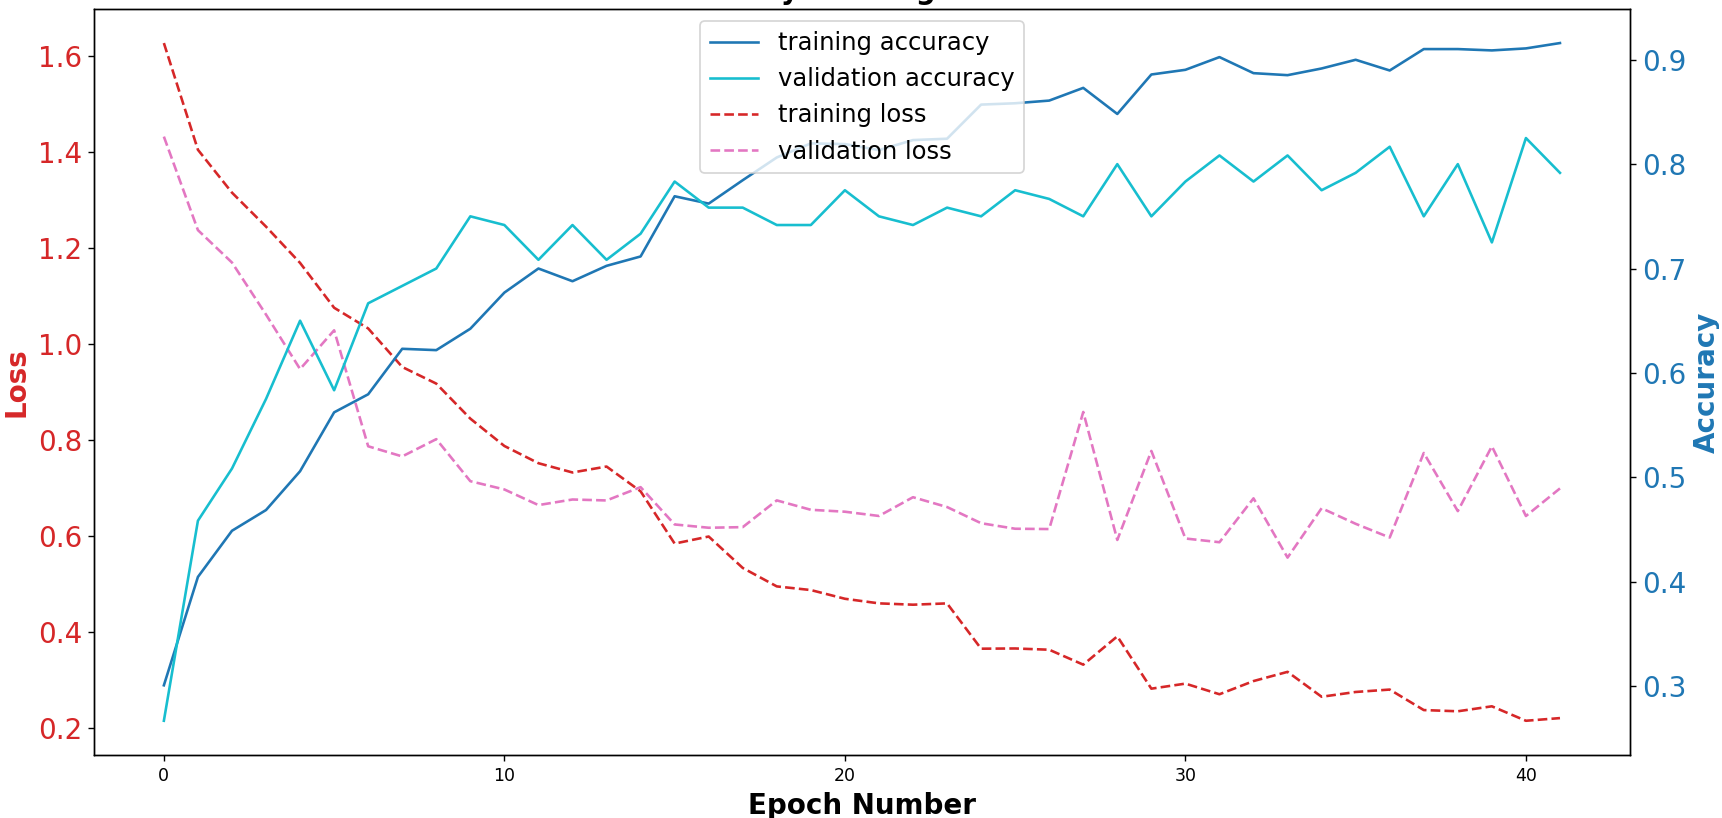
\includegraphics[width=\textwidth]{images/multitask-activity-final-test.png}
        \caption{Activity loss and accuracy plot for training and validation sets during training}
        \label{fig:multitask-activity-final-test}
    \end{subfigure}
    \qquad
    \begin{subfigure}{0.47\textwidth}
        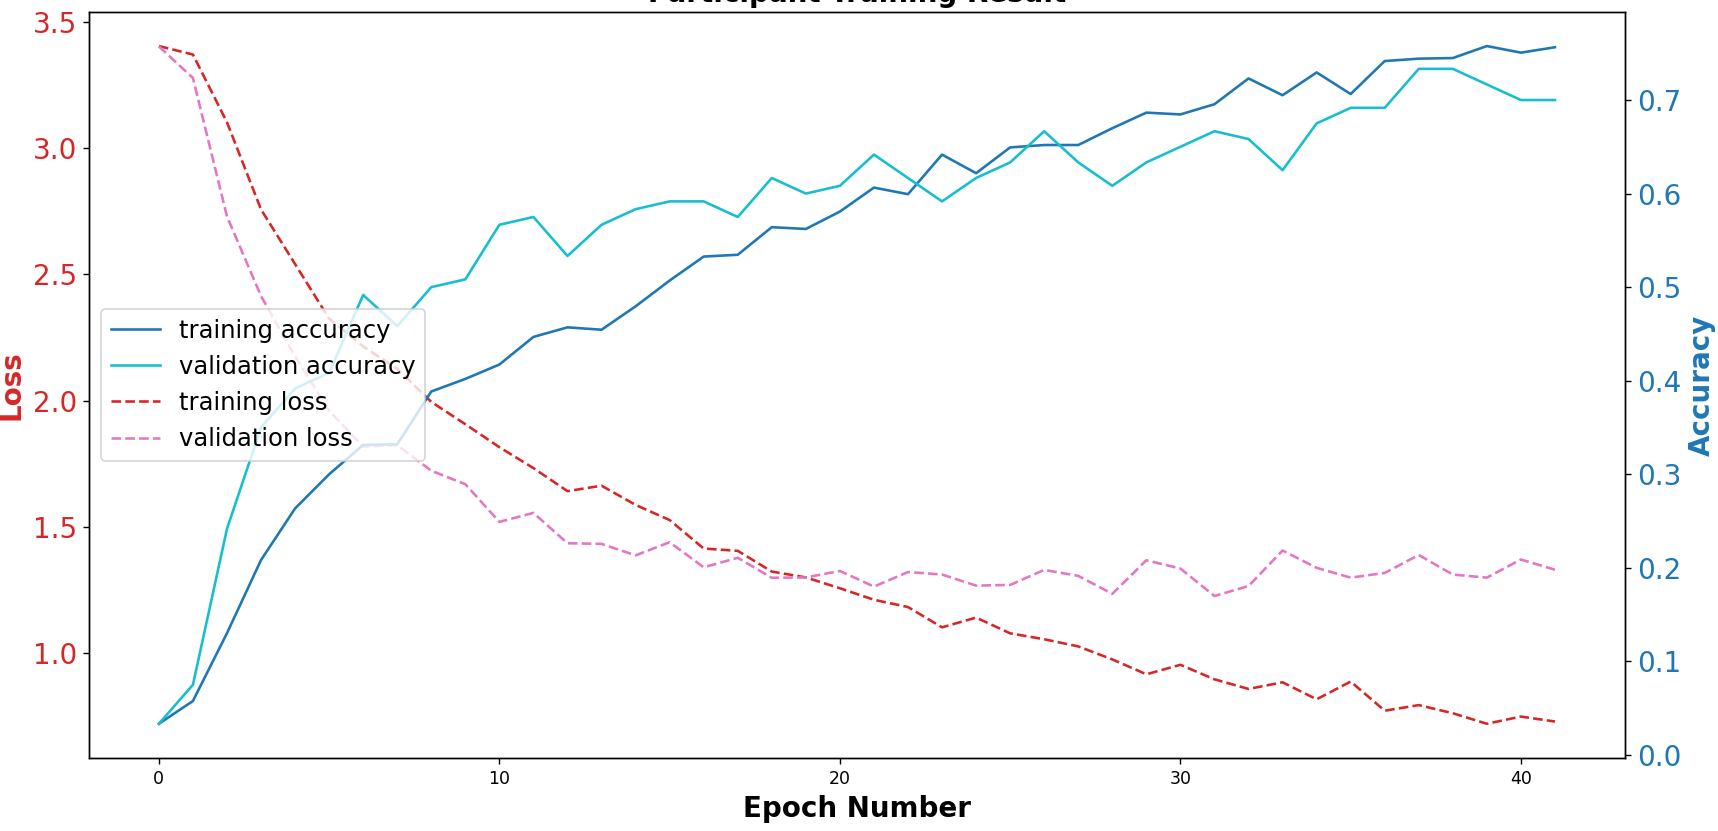
\includegraphics[width=\textwidth]{images/multitask-participant-final-test.png}
        \caption{Participant loss and accuracy plot for training and validation sets during training}
        \label{fig:multitask-participant-final-test}
    \end{subfigure}
    \caption{\subref{fig:multitask-activity-final-test} shows the activity loss and accuracy values of training and validation across running epochs. Subsequently, \subref{fig:multitask-participant-final-test} shows that of participant’s. The loss plotted lines are shown in red (training set) and pink (validation set) and the accuracy plotted lines are shown in blue (training set) and cyan (validation set).}
    \label{fig:multitask-final-loss-and-accuracy-plots}
\end{figure}

When predict with unseen test set, the model demonstrated an impressive improvement in both tasks as compared to the result from the initial CNN configuration. The activity accuracy improved to 86.67\%, with precision, recall, and F1-score increasing to 0.85, 0.87, and 0.85, respectively. Similarly, participant recognition metrics experienced noteworthy advancements, with accuracy jumping to 80.00\%, and precision, recall, and F1-score reaching 0.73, 0.80, and 0.75, respectively. The final confusion matrices of both tasks can be viewed in Figure \ref{fig:multitask-final-confusion-matrices}.

\begin{figure}[h]
   \centering
   \begin{subfigure}{0.49\textwidth}
        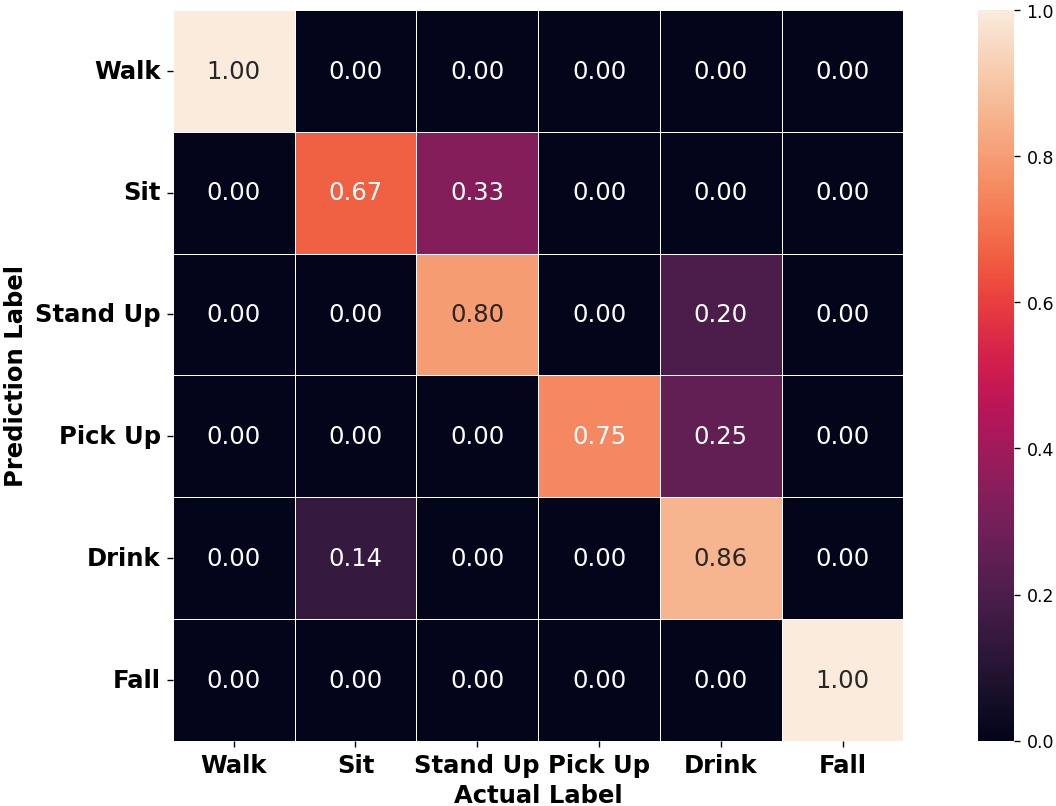
\includegraphics[width=\textwidth]{images/multitask-activity-final-test-confusion-matrix.png}
        \caption{Activity confusion matrix}
        \label{fig:multitask-activity-final-test-confusion-matrix}
    \end{subfigure}
    \qquad
    \begin{subfigure}{0.45\textwidth}
        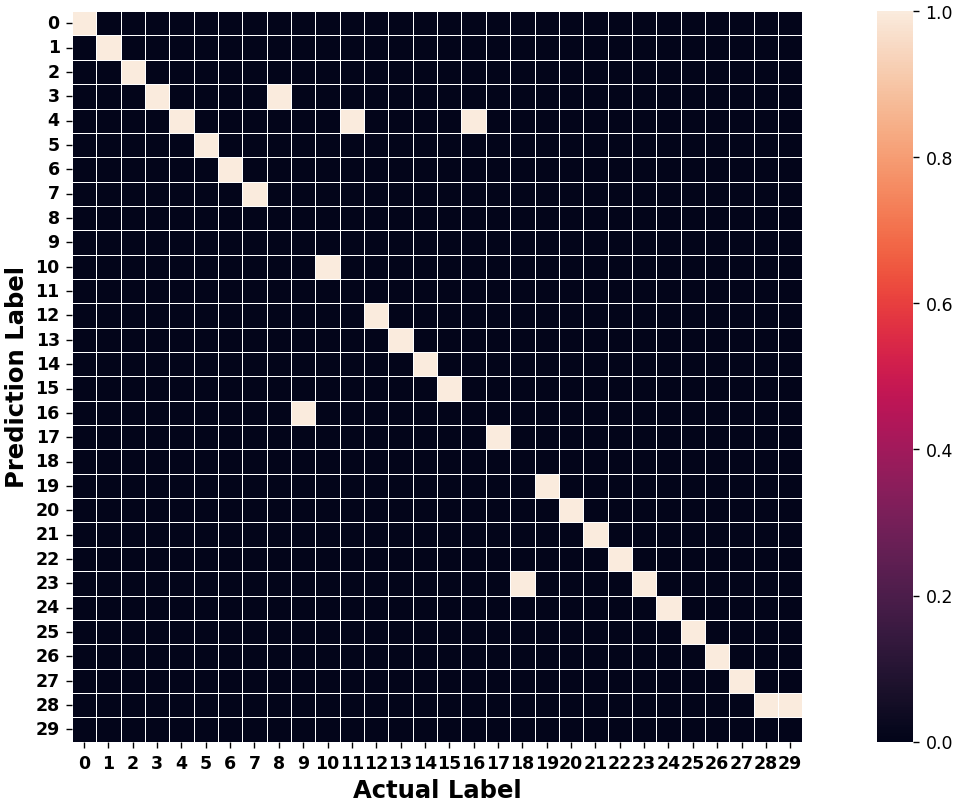
\includegraphics[width=\textwidth]{images/multitask-participant-final-test-confusion-matrix.png}
        \caption{Participant confusion matrix}
        \label{fig:multitask-participant-final-test-confusion-matrix}
    \end{subfigure}
  \caption{The figures shows the prediction performance of the optimal CNN model on the test set. \subref{fig:multitask-activity-initial-test-confusion-matrix} displays the confusion matrix of activity classification task. \subref{fig:multitask-participant-initial-test-confusion-matrix} shows the confusion matrix of participant recognition task.}
  \label{fig:multitask-final-confusion-matrices}
\end{figure}

\subsection{Result Evaluation}
The final model's performance exhibits notable enhancements across both tasks in all classification metrics compared to the initial settings. Notably, the improvements highlight a significant boost in the model's ability to accurately identify participants, a task that initially posed substantial challenges. This indicates that not only is the final model more accurate overall, but it also makes fewer mistakes in both false positives and false negatives, leading to a more reliable model. Furthermore, the model demonstrates a more balanced performance between the two tasks, indicating effective mitigation of previous imbalances. The bar charts in Figure \ref{fig:multitask-configuration-comparison} illustrate the performance comparison between baseline and optimal model configurations for the multi-task model.

\begin{figure}[h]
    \centering
    \begin{subfigure}{0.4\textwidth}
        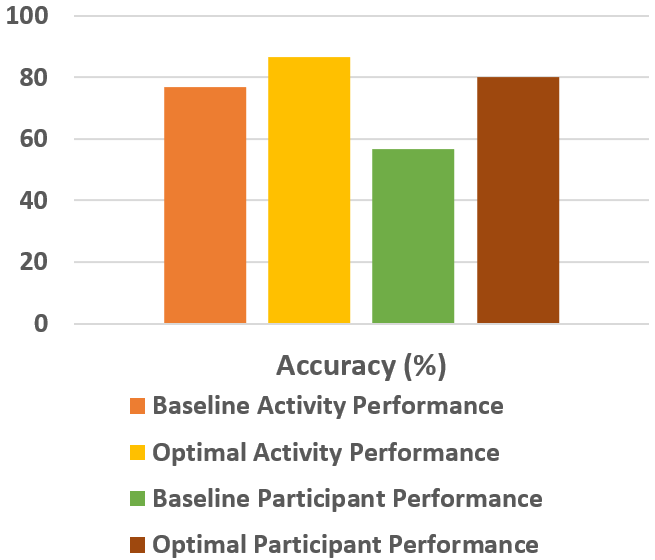
\includegraphics[width=\textwidth]{images/multitask-configuration-comparison-barchart1.png}
        \caption{Accuracy (\%)}
        \label{fig:multitask-configuration-comparison-barchart1}
    \end{subfigure}
    \qquad
    \begin{subfigure}{0.4\textwidth}
        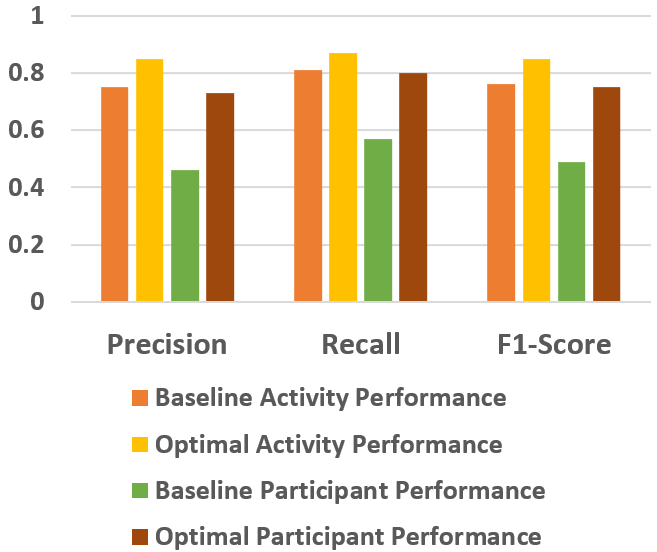
\includegraphics[width=\textwidth]{images/multitask-configuration-comparison-barchart2.png}
        \caption{Precision, Recall, F1-score}
        \label{fig:multitask-configuration-comparison-barchart2}
    \end{subfigure}
    \caption{The bar charts display the improvements in performance between baseline CNN configuration and optimal CNN configuration of multi-task network.}
    \label{fig:multitask-configuration-comparison}
\end{figure}

\subsection{Data Augmentation Evaluation}
The experiments above were conducted using axis-flipping technique. We now aim to evaluate the performance differences associated with various data augmentation techniques. Based on the data presented in Table \ref{tab:multitask-data-augmentations-evaluation}, it is evident that axis-flipping augmentation delivers the most balanced performance across tasks and also yields the best overall performance results. If prioritizing activity classification, employing mixup data augmentation emerges as the optimal choice. Conversely, for achieving high accuracy in participant identification, axis-flipping stands out as the preferred method. These findings are consistent with the optimal data augmentation strategies identified in the single-task model evaluations discussed earlier. The best overall performance results achieved include activity classification accuracy and F1-score of 90.00\% and 0.89 respectively, and participant identification accuracy and F1-score of 80.00\% and 0.73.

\subsection{Multi-task vs Single-task Comparison}
Our performance comparison is based on results obtained from the data augmentation tables, as detailed in Tables \ref{tab:activity-classification-data-augmentations-evaluation}, \ref{tab:participant-recognition-data-augmentations-evaluation}, and \ref{tab:multitask-data-augmentations-evaluation}.

Upon comparison, it is observed that the multi-task model exhibits slightly lower performance across both tasks. For instance, the single-task activity classification model achieved a peak accuracy of 96.72\% with an F1-score of 0.97, and the single-task participant identification model reached an accuracy of 86.67\% with an F1-score of 0.82. Conversely, the multi-task model's best performance was 90.00\% accuracy with an F1-score of 0.89 for the activity task, and 80.00\% accuracy with an F1-score of 0.73 for participant identification.

The disparity between the single-task and multi-task models' performance is largely due to the added complexity of balancing multiple objectives. While multi-task learning models benefit from shared representations and simplified model architecture, they tend to struggle with achieving the same levels of performance with the specialized single-task models. This trade-off highlights a balance between the efficiency of learning shared features and the precision of task-specific outcomes. However, the multi-task model's competent performance across tasks underlines its usefulness in scenarios where the balance between model efficiency and task generalization is essential.

\section{Privacy Preservation Evaluation}
We outlined our objective to preserve privacy by effectively reducing the accuracy of participant identification predictions while maintaining the efficiency of activity classification. Accordingly, our privacy requirement indicator is detailed in Equation \ref{eq:privacy_requirement_indicator}, aiming to reduce the F1-score to 0.033 or below. For evaluation, we introduced two privacy mechanisms: the standard $\epsilon$-differential privacy and Adaptive Feature-based Perturbation (which represents our proposed approach). It is important to note that our evaluation will primarily focus on the F1-score as a metric. The model diagrams illustrating both mechanisms are available in Figure \ref{fig:differential-privacy-mechanism-models} in the appendix.

\subsubsection{Multi-task Model Baseline Performance:}
The multi-task model selected for our privacy preservation experiments demonstrates a high activity recognition accuracy of 96.67\%, with precision, recall, and F1-score all closely matching at approximately 0.96. In contrast, the model's performance in participant identification shows an accuracy of 70.00\%, accompanied by precision, recall, and F1-score values of 0.58, 0.70, and 0.62, respectively. These metrics establish our baseline for scenarios where no noise is added to the data ($\epsilon=0$). Figure \ref{fig:privacy-preservation-basecase-result-evaluation} in the appendix provides the prediction plots and confusion matrices for both tasks under these conditions.

\subsubsection{Epsilon Value Iteration:} 
To fairly evaluate the effectiveness of both privacy-preserving mechanisms in maintaining utility while preserving privacy, we adopted a consistent method of assessment. The evaluation commenced with $\epsilon=0$, symbolizing the scenario of minimal privacy where no noise is introduced to obscure the data. Starting from this point, we progressively incremented the epsilon value in each iteration until meeting the privacy requirement. This methodical process enabled a comprehensive examination of various privacy levels, ranging from more lenient (lower epsilon values) to stricter (higher epsilon values).

\subsubsection{Statistical Analysis:}
For each epsilon value, we conducted ten iterations, reapplying the Laplace noise according to the chosen privacy mechanism and the current epsilon value's intensity. Subsequently, we computed the average F1-score across these ten iterations.

\subsubsection{Visualization and Trend Analysis:}
The average F1-score for each epsilon value was plotted to assess the impact levels of the privacy preservation mechanism on the model's performance. By illustrating the average F1-scores against their respective epsilon values, we aimed to reveal the trend between the participant task's prediction performance and the strength of the privacy level.

\subsection{Standard $\epsilon$-differential Privacy (DP) Mechanism}
\subsubsection{Visualization and Trend Analysis:}
$\epsilon$-DP utilizes the standard technique of applying the Laplace noise into the data. The graph in Figure \ref{fig:privacy-preservation-epsilon-evaluation-method1-f1-scores} demonstrates the impact of implementing $\epsilon$-DP. Initially, the accuracy of both tasks declines gradually, then more pronounced, before beginning to stabilize once the $\epsilon$ value exceeds 0.16. We can observe that the F1-score for participant identification meets our defined privacy requirement when $\epsilon$ reaches 0.14, with a F1-score of 0.018. At this point, the performance of activity classification has already decreased to 0.17. Compared to the baseline where $\epsilon$=0, this represents a significant drop of 82.29\% in activity classification accuracy. This underscores the need for a more effective privacy-preserving mechanism that can reduce the performance degradation in activity classification, thereby maintaining utility.

\begin{figure}[h]
    \centering
    \begin{subfigure}{1\textwidth}
    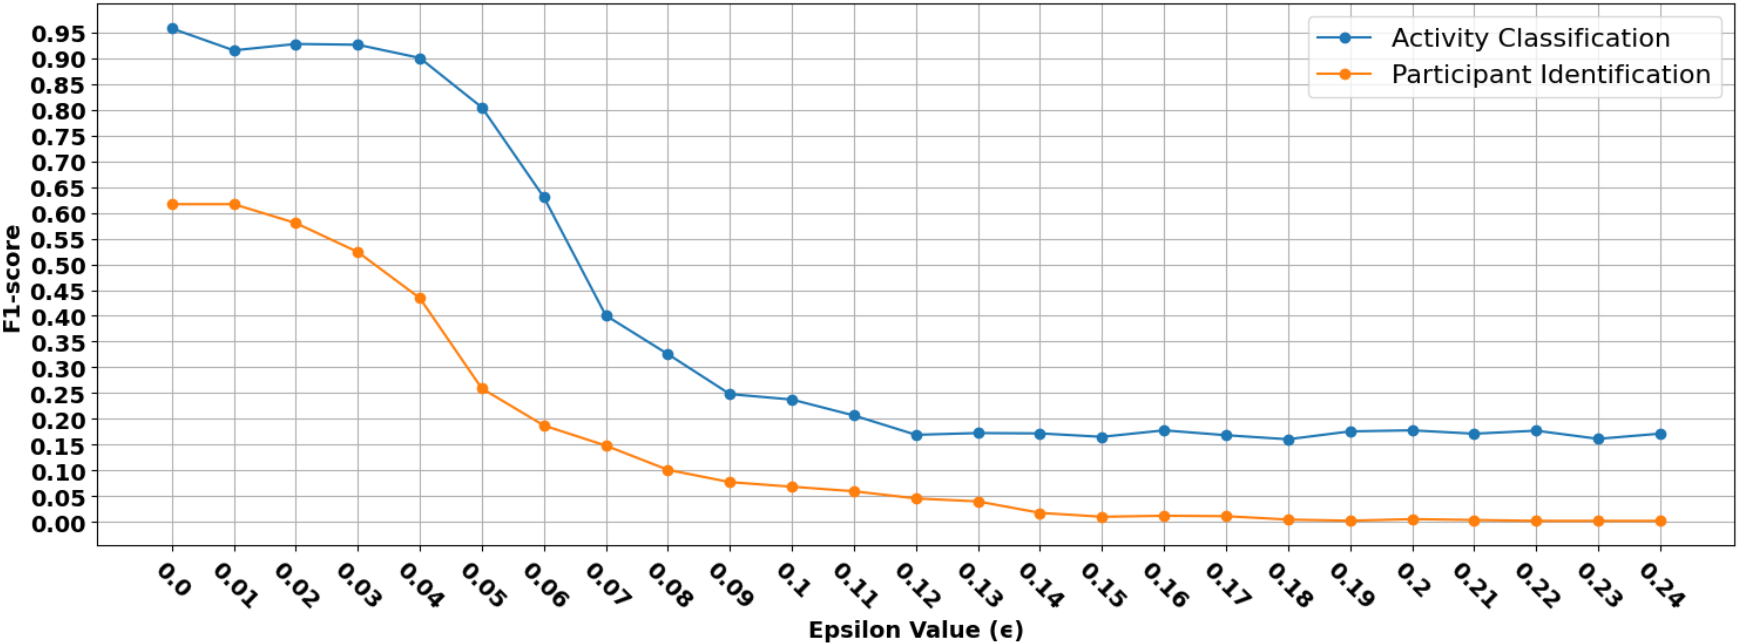
\includegraphics[width=1\linewidth]{images/privacy-preservation-epsilon-evaluation-method1-f1-scores.png}
    \caption{The graph depicts the F1-score performance across different Laplace noise strength ($\epsilon$ value).}
    \label{fig:privacy-preservation-epsilon-evaluation-method2-f1-scores-topk1000-performance-difference}
    \end{subfigure}
    \hfill
    \begin{subfigure}{0.35\textwidth}
    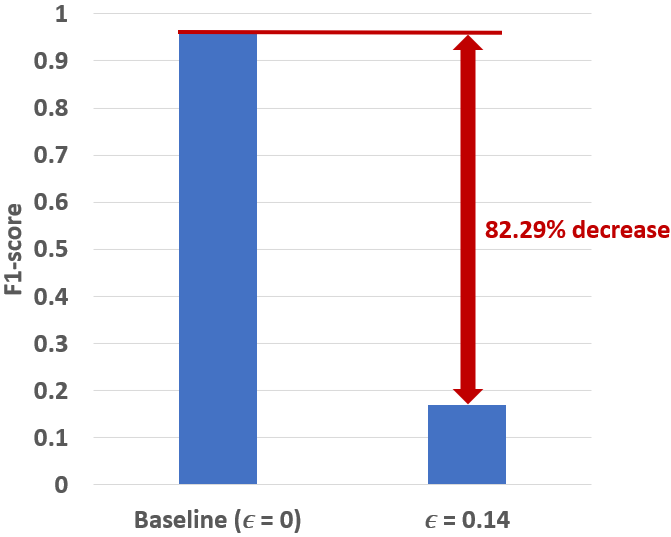
\includegraphics[width=\textwidth]{images/privacy-preservation-difference-comparison-method1-activity-f1-scores.png}
    \caption{Activity performance deterioration}
    \label{fig:privacy-preservation-difference-comparison-method1-activity-f1-scores}
    \end{subfigure}
    \qquad
    \begin{subfigure}{0.35\textwidth}
    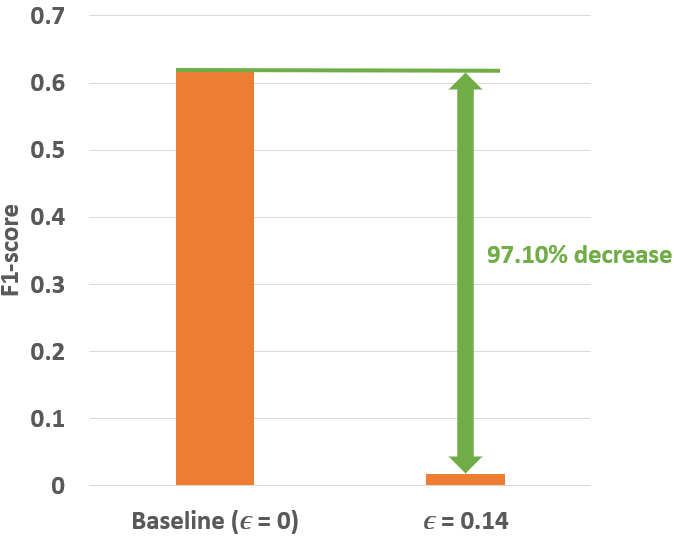
\includegraphics[width=\textwidth]{images/privacy-preservation-difference-comparison-method1-participant-f1-scores.png}
    \caption{Participant performance deterioration}
    \label{fig:privacy-preservation-difference-comparison-method1-participant-f1-scores}
    \end{subfigure}
    \caption{Figure \subref{fig:privacy-preservation-difference-comparison-method1-activity-f1-scores} shows 82.29\% reduction in activity classification performance. Figure \subref{fig:privacy-preservation-difference-comparison-method1-participant-f1-scores} shows 97.10\% reduction in participant identification performance. The results are from utilizing the standard $\epsilon$-DP mechanism.}
    \label{fig:privacy-preservation-epsilon-evaluation-method1-f1-scores}
\end{figure}

\subsubsection{Result Evaluation:}
Using the standard $\epsilon$-DP for privacy preservation significantly impacts the utility of the data. Figure \ref{fig:privacy-preservation-method1-result-evaluation}, in the appendix, shows the confusion matrices for both tasks when applying a noise strength of $\epsilon=0.14$. It is noticeable that "falling frontwards" is the only activity for which the model can maintain acceptable prediction accuracy, with 60\% of the predictions being correct. For the other activities, the model's performance significantly deteriorates, failing to predict with satisfactory accuracy.

\subsection{Adaptive Feature-based Perturbation (AFP)}
In the Adaptive Feature-based Perturbation (AFP) approach, Laplace noise is selectively added to only the top K most critical features for participant identification, as determined by the gini impurity results from a random forest analysis. 

\subsubsection{Optimal K Value Experiment:}
After resizing and normalizing, the radar data sample dimensions are 400x240. Unrolling the data reveals a total of $400 \times 240 = 96,000$ features in each radar sample. This experiment aimed to identify the optimal number of top K features critical for participant identification while minimally impacting the performance of the activity classification task. Achieving this balance is crucial for meeting privacy requirements without significantly compromising the utility seen in the $\epsilon$-DP mechanism results.

The initial experiment began with an extensive analysis to determine the most beneficial range within the top 10,000 features. This phase involved incrementally increasing K, starting from 1,000 and rising by 1,000 in each iteration up to K=10,000. This process set a baseline for identifying a more precise range that could potentially determine the optimal K value. Following this, we conducted a detailed examination through a nested loop, varying $\epsilon$ value strengths from 0 to 0.9, in increments of 0.03, to evaluate the differential privacy's impact on both tasks' F1-scores across different K values.

Figure \ref{fig:privacy-preservation-topk10000-evaluation}, in the appendix, presents the initial experiment's outcome, indicating that K=1000 achieves the best balance between privacy and performance. The activity classification task's performance accuracy is notably best at K=1000, as shown in the sub-figure \subref{fig:privacy-preservation-topk10000-evaluation-method2-activity-f1-scores}. Other K values demonstrated significantly poorer performance. Meanwhile, the participant task's sub-figure \subref{fig:privacy-preservation-topk10000-evaluation-method2-participant-f1-scores} shows that while the F1-score's decline for K=1000 is initially more gradual compared to other K values, it converges to a similar level when $\epsilon$ exceeds 0.78.

A subsequent, more focused analysis explored the range from K=100 to K=1000 in increments of 100, employing a similar nested loop to assess differential privacy's effects. Despite this detailed exploration, the results consistently affirmed K=1000 as the optimal choice for balancing participant identification privacy with activity classification performance. Figure \ref{fig:privacy-preservation-topk1000-evaluation}, in the appendix, showcases the experimentation results. 
In the activity sub-figure \subref{fig:privacy-preservation-topk1000-evaluation-method2-activity-f1-scores}, we observe that the highest F1-score performance from $\epsilon=0.81$ onwards is achieved by applying noise to the top $K=100$ and $K=1000$ features. Examining the participant sub-figure \subref{fig:privacy-preservation-topk1000-evaluation-method2-participant-f1-scores}, it becomes apparent that applying noise to the top $K=100$ features does not suffice to meet the privacy requirement, as the F1-score is 0.26 when $\epsilon=0.90$. However, focusing on the F1-score for the top $K=1000$, we notice that it meets the privacy requirement after it reaches $\epsilon=0.81$. This clearly demonstrating that K=1000 not only sustains the best performance in activity classification but also significantly reduces participant identification's effectiveness.

\subsubsection{Visualization and Trend Analysis:}
The graph depicted in Figure \ref{fig:privacy-preservation-evaluation-and-difference-comparison} demonstrates the performance trends of both tasks, illustrating how the F1-score for participant identification declines more sharply compared to that of activity classification. This pattern of differential degradation aligns with expectations since the noise addition is specifically aimed at participant-related features.

As the epsilon value increases, the F1-score for the participant identification task decreases sharply, reaching a low of 0.01 at $\epsilon = 0.81$, thereby fulfilling the set privacy-preserving criteria for this experiment. At this point, the F1-score for the activity classification task is at 0.67, showing a decrease of 30.21\% from its initial value of 0.96 at $\epsilon = 0$. In contrast, the participant identification task experiences a more significant drop, from an initial F1-score of 0.62 down to 0.01, representing a 98.39\% reduction. This disparity in decline rates between the two tasks highlights the AFP strategy's effectiveness. Figures \subref{fig:privacy-preservation-difference-comparison-method2-activity-f1-scores} and \subref{fig:privacy-preservation-difference-comparison-method2-participant-f1-scores} in Figure \ref{fig:privacy-preservation-evaluation-and-difference-comparison} visualize these results.

Furthermore, Figure \subref{fig:privacy-preservation-epsilon-evaluation-method2-f1-scores-topk1000-performance-difference} illustrates that the addition of minimal Laplace noise to the dataset can actually improve the performance of the activity classification task, achieving an F1-score of 1.00. This enhancement indicates that the introduction of slight noise can assist in the generalization and robustness of the data. Consequently, this might help the trained model to achieve better prediction performance, as the noise serves as a form of regularization.

\subsubsection{Result Evaluation}
Figure \ref{fig:privacy-preservation-method2-result-evaluation}, in the appendix, displays the confusion matrices for both tasks after applying Laplace noise to the top 1000 features that are critical for participant identification, using an epsilon value of 0.81. It is notable that, despite a decrease in the overall performance of activity prediction, the model still achieved 100\% accuracy in classifying specific activities such as standing up, drinking from a glass, and falling forwards. The activity that experienced the most significant decline in classification accuracy is "picking up an object," with only 33\% of predictions being correct.

\subsection{Privacy-preservation Mechanism Comparison}
Based on the results of both privacy-preservation mechanisms, $\epsilon$-DP and the proposed AFP, we observe a notable improvement in classification accuracy. Upon meeting the privacy requirement, the activity classification F1-score for $\epsilon$-DP stands at 0.17, whereas for AFP stands at 0.67. This indicates that AFP minimizes the deterioration impact on data utility much better, with 50\% more accurate. This performance disparity is depicted in Figure \ref{fig:privacy-preservation-evaluation-and-difference-comparison-method1-and-method2}, in the appendix. It is also worth noting that AFP requires a higher $\epsilon$ value to achieve the privacy requirement compared to $\epsilon$-DP; $\epsilon$-DP reaches the privacy criterion at $\epsilon=0.14$, while AFP requires $\epsilon=0.81$. This difference is anticipated since AFP applies noise to only 1000 features, necessitating a greater strength of noise to fulfill the privacy requirement. Conversely, $\epsilon$-DP distributes noise across all features, thus requiring a lower $\epsilon$ value to meet the same criterion.

\begin{figure}[h]
    \centering
    \begin{subfigure}{1\textwidth}
    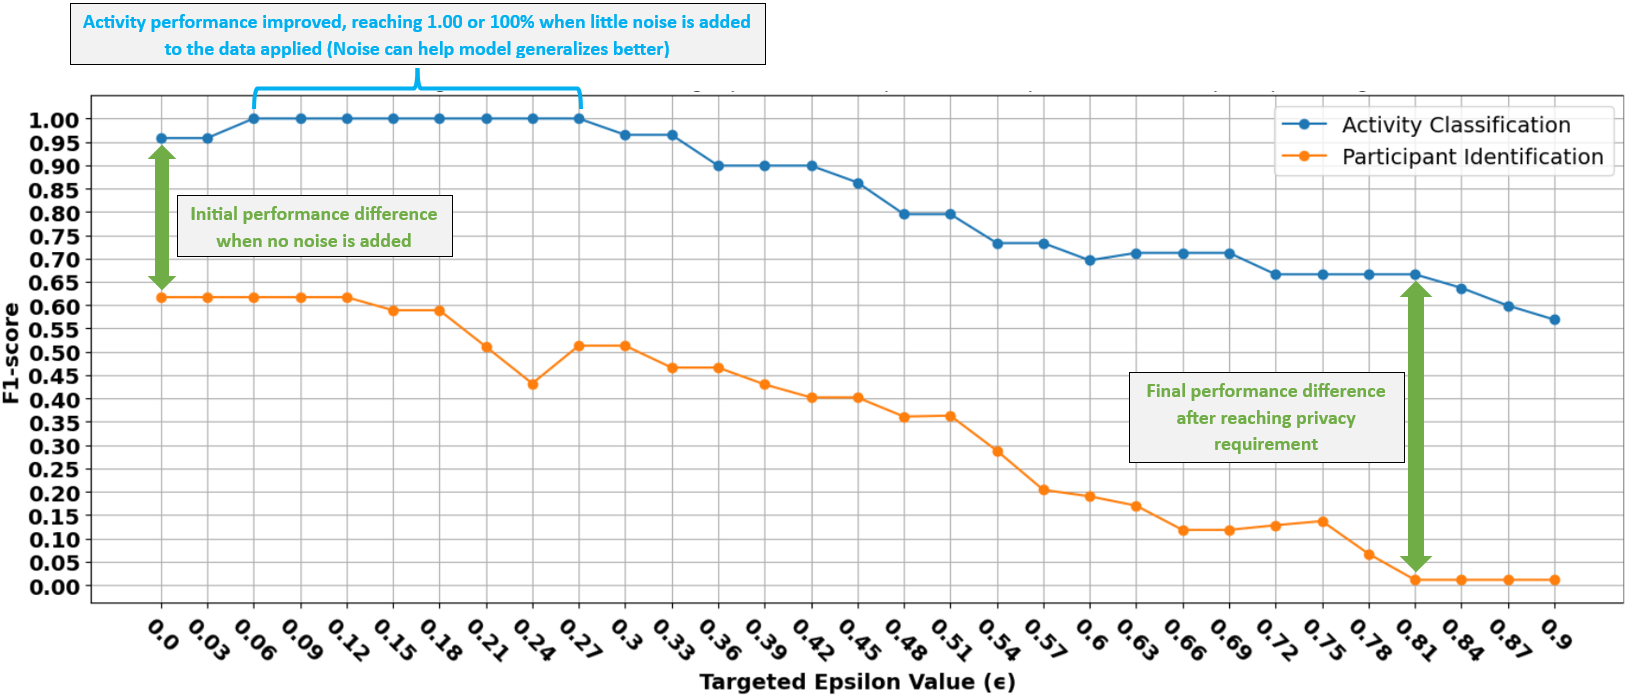
\includegraphics[width=\textwidth]{images/privacy-preservation-epsilon-evaluation-method2-f1-scores-topk1000-performance-difference.png}
    \caption{The graph depicts the F1-score performance across different Laplace noise strength ($\epsilon$ value).}
    \label{fig:privacy-preservation-epsilon-evaluation-method2-f1-scores-topk1000-performance-difference}
    \end{subfigure}
    \hfill
    \begin{subfigure}{0.35\textwidth}
    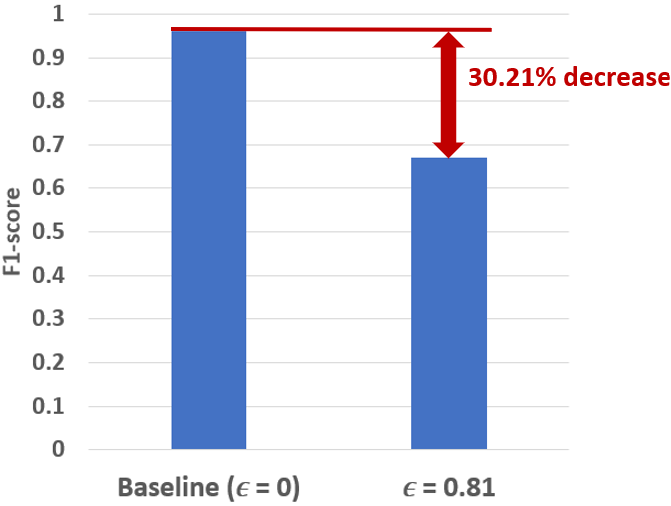
\includegraphics[width=\textwidth]{images/privacy-preservation-difference-comparison-method2-activity-f1-scores.png}
    \caption{Activity performance deterioration}
    \label{fig:privacy-preservation-difference-comparison-method2-activity-f1-scores}
    \end{subfigure}
    \qquad
    \begin{subfigure}{0.35\textwidth}
    \includegraphics[width=\textwidth]{images/privacy-preservation-difference-comparison-method2-participant-f1-scores.png}
    \caption{Participant performance deterioration}
    \label{fig:privacy-preservation-difference-comparison-method2-participant-f1-scores}
    \end{subfigure}
    \caption{\subref{fig:privacy-preservation-difference-comparison-method2-activity-f1-scores} shows 30.21\% reduction in activity classification performance. \subref{fig:privacy-preservation-difference-comparison-method2-participant-f1-scores} shows 98.39\% reduction in participant identification performance. The results are from utilizing the proposed AFP mechanism on Top K=1000 features of participant identification.}
    \label{fig:privacy-preservation-evaluation-and-difference-comparison}
\end{figure}


%==================================================================================================================================
\chapter{Conclusion}

In the healthcare industry, analyzing human motion offers significant insights into the detection of movement abnormalities and the progression of neurological conditions, such as Parkinson's and Alzheimer's, in patients. Advances in machine learning have paved the way for intelligent systems capable of performing at or above human levels in these applications. Nonetheless, applying these advancements within healthcare poses considerable challenges, including ethical issues and privacy concerns, which must be thoroughly addressed before widespread implementation.

This study aimed to investigate, develop, and propose a privacy-preserving mechanism for using radar data for Human Activity Recognition (HAR). To ensure structured progress towards our objective, we established milestones to monitor our project's development. Initially, our efforts were focused on training single-task convolutional neural network (CNN) models to classify activities and identify participants from radar samples. Subsequently, we ventured into integrating these models into a multi-task CNN framework, capable of simultaneously addressing both tasks.

Our evaluations indicate that while the multi-task model marginally underperformed in both activity classification and participant identification tasks compared to the dedicated single-task models, its ability to strike a balance between model efficiency and task generalization remains advantageous. The slight dip in multi-task model performance is largely due to the complexities of optimizing multiple objectives simultaneously. Despite this, multi-task learning models benefit from shared representations. This minor performance trade-off highlights a compromise between learning efficiency and the accuracy of task-specific outcomes. Yet, the multi-task model's capacity to achieve respectable results across both tasks with a unified architecture demonstrates its value, particularly in scenarios where compactness and versatility across tasks are critical.

In addressing our primary objective of proposing a privacy-preserving mechanism, we commenced by identifying a threat model scenario pertinent to our task. Our privacy requirement was determined based on the likelihood of correctly guessing a participant's label by chance. We explored two privacy preservation methods. The first, standard $\epsilon$-differential privacy ($\epsilon$-DP), involved applying Laplace noise across all features of the data. This approach is advantageous in preserving privacy, however it fell short of balancing privacy and classification efficiency as it severely deteriorate the impact on the classification task. Our second method, the Adaptive Feature-based Perturbation (AFP), proposed a targeted approach of applying Laplace noise to the top K most critical features for participant identification, determined using the gini impurity technique from training random forest model. Our evaluations found that the optimal K value is 1000, striking a balance between meeting our privacy requirements and maintaining robust activity classification performance.

The AFP mechanism proved to be a satisfactory solution for our study, effectively preserving privacy by limiting the model's ability to accurately predict participant identities beyond our established privacy threshold. Moreover, it did so without significantly affecting the activity classification task's performance. Our results demonstrate that the AFP mechanism can reduce the accuracy of the participant identification task by 98.39\% to meet the set privacy requirements, while the impact on activity classification performance is limited to a decrease of only 30.21\%. In comparison to the results obtained using $\epsilon$-DP, the AFP mechanism facilitated a notable 50\% improvement in the model's activity classification capability. This represents a significant enhancement in performance, emphasizing the AFP mechanism's effectiveness in balancing privacy preservation with maintaining task utility.

In conclusion, our investigation into privacy-preserving mechanisms, specifically within the radar data, marks a significant advancement in addressing the privacy and ethical concerns that impede the application of deep learning in healthcare. Through this study, the AFP mechanism has emerged as a promising strategy that seeks to reconcile these considerations, demonstrating the potential for machine learning models to be sensitively adapted for healthcare applications. This approach not only enhances the privacy of individuals but also maintains the utility of the data for meaningful analysis, paving the way for future research to further refine and implement such privacy-preserving techniques in real-world scenarios.

\subsubsection{Limitations:}
A significant challenge encountered in this project was the hardware limitations, particularly in terms of RAM and storage capacity. Processing the extensive size of the original radar dataset required substantial RAM, leading to frequent crashes due to insufficient memory on our local computing resources. To address this, we were compelled to downsample the data to one-sixteenth of its original size, allowing us to train our CNN models within the limits of our local systems. Although necessary, this reduction prompts questions regarding the potential loss of critical information and its unclear impact on the study's outcomes. Additionally, our hardware limitations restricted our ability to fully leverage some memory-intensive deep learning frameworks, such as Optuna for comprehensive hyperparameter tuning and SHAP for more effective feature extraction. These tools could have potentially enhanced model's classification performances and further mitigated the impact on activity classification during the evaluation of our proposed AFP method for privacy preservation. Despite these obstacles, we managed to navigate these limitations and achieve commendable outcomes. The project's success, amidst such constraints, underscores our adaptability and capacity to produce significant results.

\subsubsection{Future Works:}
Exploring alternative privacy-preserving techniques represents a promising avenue for future studies. One such technique uses Autoencoder-based Anonymization, which employs autoencoders to learn a new representation of the data. This approach could be aimed to retain critical features necessary for accurately classifying activities while effectively masking features that could reveal participant identities. By transforming data in this manner, it is possible to safeguard privacy without compromising the utility for its intended application.

GANs offer another promising and innovative approach. The development of GANs to generate synthetic radar data samples presents an intriguing opportunity. These synthetic samples, designed to be indistinguishable from real radar data but do not carry participants' identifiable information, could significantly mitigate privacy concerns. By ensuring these generated samples do not contain identifiable information, GANs could serve as a powerful tool in preserving privacy while maintaining the quality of data analysis.

Additionally, revisiting the impact of data quality on the research outcomes could peak interest for further investigation. Our study necessitated the downsizing of data samples, which could lead to some loss of critical information. Future studies could explore the effects of utilizing the original dataset quality, then comparing the results with those obtained from downsampled datasets. Future work could delve into the use of more memory-intensive deep learning frameworks, such as Optuna and SHAP. This could assess their effectiveness in enhancing classification tasks and in improving the efficacy of the proposed AFP mechanism.

Nevertheless, the insights from this study remarkably contribute to the ongoing discussion on privacy within healthcare analytics and establish a groundwork for future research focused on refining and applying privacy-preserving mechanisms to radar data. Through continuous exploration, subsequent research will undoubtedly advance our capacity to safeguard individual privacy while utilizing data for meaningful healthcare improvements. Eventually, radar technology may emerge as a preferable option for maintaining privacy, finding its place in the healthcare industry for patient monitoring, aligning with the objectives outlined in this study.
%==================================================================================================================================
%
% 
%==================================================================================================================================
%  APPENDICES  

\begin{appendices}
% \newgeometry{bottom=1cm, footskip=.5cm}

\chapter{Appendices}

\section{Radar Dataset Graph}
\begin{figure}[h]
   \centering
   \begin{subfigure}[b]{0.43\textwidth}
        \includegraphics[width=\textwidth]{images/dataset-march2017.png}
        \caption{March 2017}
        \label{fig:dataset-march2017}
    \end{subfigure}
    \hfill
    \begin{subfigure}[b]{0.43\textwidth}
        \includegraphics[width=\textwidth]{images/dataset-june2017.png}
        \caption{June 2017}
        \label{fig:dataset-june2017}
    \end{subfigure}
    \hfill
    \begin{subfigure}[b]{0.43\textwidth}
        \includegraphics[width=\textwidth]{images/dataset-december2017.png}
        \caption{December 2017}
        \label{fig:dataset-december2017}
    \end{subfigure}
    \hfill
    \begin{subfigure}[b]{0.43\textwidth}
        \includegraphics[width=\textwidth]{images/dataset-july2018.png}
        \caption{July 2018}
        \label{fig:dataset-july2018}
    \end{subfigure}
    \hfill
    \begin{subfigure}[b]{0.43\textwidth}
        \includegraphics[width=\textwidth]{images/dataset-february2019.png}
        \caption{February 2019 (NG Homes)}
        \label{fig:dataset-february2019}
    \end{subfigure}
    \hfill
    \begin{subfigure}[b]{0.43\textwidth}
        \includegraphics[width=\textwidth]{images/dataset-february2019_2.png}
        \caption{February 2019 (West Cumbria)}
        \label{fig:dataset-february2019_2}
    \end{subfigure}
    \hfill
    \begin{subfigure}[b]{0.43\textwidth}
        \includegraphics[width=\textwidth]{images/dataset-march2019.png}
        \caption{March 2019}
        \label{fig:dataset-march2019}
    \end{subfigure}
  \caption{The bar charts show the total number of radar files per participant ID of each experimentation date. There is a maximum of 18 files per participant (representing 6 activities and 3 repetitions).}
  \label{fig:full-dataset-information}
\end{figure}

\newpage

\section{Full Radar Dataset Table Summary}
\begin{table}[h]
    \centering
    \begin{tabular}{|c|p{2.5cm}|c|c|c|c|c|}
        \hline
        \rowcolor{lightgray}
        \textbf{No.} & \textbf{Date} & \textbf{Location} & \textbf{Activities} & \textbf{Participants} & \textbf{Rep.} & \textbf{Files} \\
        \hline
        1 & March 2017 & N/A & 6 & 4 & 2 & 48 \\
        \hline
        2 & June 2017 & N/A & 6 & 9 & 3 & 162 \\
        \hline
        3 & December 2017 & University of Glasgow laboratory room & 6 & 20 & 3 & 360 \\
        \hline
        4 & July 2018 & University of Glasgow common room & 6 & 16 & 3 & 288 \\
        \hline
        5 & February 2019 & University of Glasgow laboratory room & 6 & 17 & 3 & 306 \\
        \hline
        6 & February 2019 & Glasgow NG Homes Room 1 to 3 & 5 & 20 & 3 & 301 \\
        \hline
        7 & March 2019 & Age UK West Cumbria Room 1 to 3 & 5 & 20 & 3 & 289 \\
        \hline
    \end{tabular}
    \caption{Summary of the radar dataset detail, categorized by the date of experiment. Within the table shows the location and the number of activities, participants, repetitions (Rep.), and files recorded.}
    \label{tab:dataset-details}
\end{table}

\section{Raw Captured Radar Data plots}
\begin{figure}[h]
   \centering
   \begin{subfigure}[b]{0.32\textwidth}
        \includegraphics[width=\textwidth]{images/raw_data1.png}
        \caption{Walking}
        \label{fig:raw_data1}
    \end{subfigure}
    \hfill
    \begin{subfigure}[b]{0.32\textwidth}
        \includegraphics[width=\textwidth]{images/raw_data2.png}
        \caption{Sitting down}
        \label{fig:raw_data2}
    \end{subfigure}
    \hfill
    \begin{subfigure}[b]{0.32\textwidth}
        \includegraphics[width=\textwidth]{images/raw_data3.png}
        \caption{Standing up}
        \label{fig:raw_data3}
    \end{subfigure}
    \hfill
    \begin{subfigure}[b]{0.32\textwidth}
        \includegraphics[width=\textwidth]{images/raw_data4.png}
        \caption{Picking up an object}
        \label{fig:raw_data4}
    \end{subfigure}
    \hfill
    \begin{subfigure}[b]{0.32\textwidth}
        \includegraphics[width=\textwidth]{images/raw_data5.png}
        \caption{Drinking from a glass}
        \label{fig:raw_data5}
    \end{subfigure}
    \hfill
    \begin{subfigure}[b]{0.32\textwidth}
        \includegraphics[width=\textwidth]{images/raw_data6.png}
        \caption{Falling frontwards}
        \label{fig:raw_data6}
    \end{subfigure}
  \caption{Raw data plots for each of the six activities. The plots represent the magnitude of the radar signals over sample index. The number 1e6 in the x-label of figures \subref{fig:raw_data1} and \subref{fig:raw_data2} represents ${10^6}$.}
  \label{fig:raw_data_plots}
\end{figure}

\newpage

\section{Normalized and Resized Radar Sample}
\begin{figure}[h]
   \centering
   \begin{subfigure}[b]{0.4\textwidth}
        \includegraphics[width=\textwidth]{images/Velocity-Time_1.png}
        \caption{Walking}
        \label{fig:velocity-time1-1}
    \end{subfigure}
    \qquad
    \qquad
    \begin{picture}(0,0)
        \put(-35,85){\vector(1,0){30}}
    \end{picture}
    \begin{subfigure}[b]{0.4\textwidth}
        \includegraphics[width=\textwidth]{images/Velocity-Time_1_normalized_resized.png}
        \caption{Walking (Normalized and Resized)}
        \label{fig:velocity-time1-normalized-resized}
    \end{subfigure}
    \begin{subfigure}[b]{0.4\textwidth}
        \includegraphics[width=\textwidth]{images/Velocity-Time_1_normalized.png}
        \caption{Walking (Normalized)}
        \label{fig:velocity-time1-normalized}
    \end{subfigure}
    \qquad
    \qquad
    \begin{subfigure}[b]{0.4\textwidth}
        \includegraphics[width=\textwidth]{images/Velocity-Time_1_resized.png}
        \caption{Walking (Resized)}
        \label{fig:velocity-time1-resized}
    \end{subfigure}
    
  \caption{\subref{fig:velocity-time1-normalized-resized} shows the data after being normalized and resized. It can be noticed that the amplitude range has been re-scaled and the y-axis has been squeezed. \subref{fig:velocity-time1-normalized} illustrates when the data is only normalized. Subsequently, \subref{fig:velocity-time1-resized} illustrates the data when it is only resized.}
  \label{fig:Normalized Resized Comparison Plots}
\end{figure}

\newpage

\section{Classification Task Data Tables}

\subsection{Activity Classification Data Table}
\begin{table}[h]
    \centering
    \begin{tabular}{|l|c|c|c|}
        \hline
        \rowcolor{lightgray}
        \textbf{Activity} & \textbf{106-participant Dataset} & \textbf{61-participant Dataset} & \textbf{30-participant Dataset}\\
        \hline
        Walking & 312 & 183 & 90\\
        \hline
        Sitting down & 312 & 183 & 90\\
        \hline
        Standing up & 311 & 183 & 90\\
        \hline
        Picking up an object & 183 & 3 & 90\\
        \hline
        Drinking from a glass & 183 & 3 & 90\\
        \hline
        Falling frontwards & 197 & 183 & 90\\
        \hline
        Total & 1752 & 1098 & 540\\
        \hline
    \end{tabular}
    \caption{Number of data samples of each of the activity across different dataset type. These data samples are used in activity classification model training.}
    \label{tab:activity-classification-number-of-samples}
\end{table}

\subsection{Participant Identification Data Table}
\begin{table}[h]
    \centering
    \begin{tabular}{|l|c|c|c|}
        \hline
        \rowcolor{lightgray}
        \textbf{Dataset Type} & \textbf{No. of participants} & \textbf{No. of data per participant} & \textbf{Total data samples}\\
        \hline
        61-participant Dataset & 61 & 18 & 1098\\
        \hline
        30-participant Dataset & 30 & 18 & 540\\
        \hline
    \end{tabular}
    \caption{Number of data samples of each dataset type used for participant identification model training.}
    \label{tab:participant-identification-number-of-samples}
\end{table}

\subsection{Participant Identification by Activity Data Table (61-participant)}
\begin{table}[h]
    \centering
    \begin{tabular}{|l|c|c|c|}
        \hline
        \rowcolor{lightgray}
        \textbf{Activity} & \textbf{No. of participants} & \textbf{No. of data per participant} & \textbf{Total data samples}\\
        \hline
        Walking & 61 & 3 & 183\\
        \hline
        Sitting down & 61 & 3 & 183\\
        \hline
        Standing up & 61 & 3 & 183\\
        \hline
        Picking up an object & 61 & 3 & 183\\
        \hline
        Drinking from a glass & 61 & 3 & 183\\
        \hline
        Falling frontwards & 61 & 3 & 183\\
        \hline
        Total & - & - & 1098\\
        \hline
    \end{tabular}
    \caption{Number of data samples of each of the activity for 61-participant dataset for participant identification model training experiment based on each activity.}
    \label{tab:participant-identification-by-activity}
\end{table}

\newpage

\section{Data Augmentation Algorithms}
\subsection{Axis-flipping Augmentation}
\begin{algorithm}[h]
    \DontPrintSemicolon
    \KwData{$train\_data$, an array of training data.}
    \KwResult{Augmented $train\_data$ array with flipped versions of the original images: left-right flips, up-down flips, and diagonal flips.}
    \Begin{
        $train\_data\_fliplr \longleftarrow []$\;
        $train\_data\_flipud \longleftarrow []$\;
        $train\_data\_fliplr\_flipud \longleftarrow []$\;
        \For{$d \in train\_data$}
        {
            append $\text{np.fliplr}(d)$ to $train\_data\_fliplr$\;
            append $\text{np.flipud}(d)$ to $train\_data\_flipud$\;
            append $\text{np.fliplr}(\text{np.flipud}(d))$ to $train\_data\_diagonal$\;
        }
        $train\_data\_fliplr \longleftarrow \text{np.array}(train\_data\_fliplr)$\;
        $train\_data\_flipud \longleftarrow \text{np.array}(train\_data\_flipud)$\;
        $train\_data\_diagonal \longleftarrow \text{np.array}(train\_data\_diagonal)$\;
        $train\_data \longleftarrow \text{np.concatenate}((train\_data, train\_data\_fliplr))$\;
        $train\_data \longleftarrow \text{np.concatenate}((train\_data, train\_data\_flipud))$\;
        $train\_data \longleftarrow \text{np.concatenate}((train\_data, train\_data\_diagonal))$\;
    }
    
\caption{This algorithm adds horizontal, vertical, and diagonal flipped versions of the input dataset, quadrupling its size for data augmentation purposes.}
\label{alg:axis-flipping_augmentation}
\end{algorithm}

\subsection{Mixup Augmentation}
\begin{algorithm}[h]
    \DontPrintSemicolon
    \KwIn{$x$, radar samples for the batch of data; $y$, labels for the batch of data; $\alpha$, parameter of the Beta distribution used to generate mixup coefficients (default $0.2$).}
    \KwOut{$mixed\_x$, mixed input features; $mixed\_y$, mixed labels.}
    \Begin{
        \eIf{$\alpha > 0$}
        {
            $\lambda \longleftarrow \text{np.random.beta}(\alpha, \alpha)$\;
        }
        {
            $\lambda \longleftarrow 1$\;
        }
        $batch\_size \longleftarrow x.shape[0]$\;
        $index \longleftarrow \text{np.random.permutation}(batch\_size)$\;
        $mixed\_x \longleftarrow \lambda \times x + (1 - \lambda) \times x[index, :]$\;
        $mixed\_y \longleftarrow \lambda \times y + (1 - \lambda) \times y[index, :]$\;
        \Return{$mixed\_x, mixed\_y$}\;
    }
    
\caption{The algorithm mixes pairs of radar samples and their labels within a batch of data, based on coefficients drawn from the Beta distribution.}
\label{alg:mixup_data_augmentation}
\end{algorithm}

\newpage

\section{Data Augmentation Visualisation}
\subsection{Axis-flipping Augmentation}
\begin{figure}[h]
   \centering
   \begin{subfigure}[b]{0.35\textwidth}
        \includegraphics[width=\textwidth]{images/Velocity-Time_1_normalized_resized.png}
        \caption{Walking (Original)}
        \label{fig:velocity-Time_1_normalized_resized}
    \end{subfigure}
    \qquad
    \begin{subfigure}[b]{0.35\textwidth}
        \includegraphics[width=\textwidth]{images/Velocity-Time_1_normalized_resized-horizontal-flip.png}
        \caption{Walking (Horizontal)}
        \label{fig:velocity-Time_1_normalized_resized-horizontal-flip}
    \end{subfigure}
    \qquad
    \begin{subfigure}[b]{0.35\textwidth}
        \includegraphics[width=\textwidth]{images/Velocity-Time_1_normalized_resized-vertical-flip.png}
        \caption{Walking (Vertical)}
        \label{fig:velocity-Time_1_normalized_resized-vertical-flip}
    \end{subfigure}
    \qquad
    \begin{subfigure}[b]{0.35\textwidth}
        \includegraphics[width=\textwidth]{images/Velocity-Time_1_normalized_resized-diagonal-flip.png}
        \caption{Walking (Diagonal)}
        \label{fig:velocity-Time_1_normalized_resized-diagonal-flip}
    \end{subfigure}
  \caption{The plots illustrate the axis-flipping augmentation applied to walking data. Figure \subref{fig:velocity-Time_1_normalized_resized-horizontal-flip} demonstrates horizontal flipping, Figure \subref{fig:velocity-Time_1_normalized_resized-vertical-flip} displays vertical flipping, and Figure \subref{fig:velocity-Time_1_normalized_resized-diagonal-flip} showcases diagonal flipping.}
  \label{fig:Axis-flipping Plots}
\end{figure}

\subsection{Mixup Augmentation}
\begin{figure}[h]
    \centering
    \includegraphics[width=0.93\linewidth]{images/mixup_augmentation.png}
    \caption{The figure presents an example of linear interpolation between two radar activities: walking and standing up, with the array below each activity indicating its label. The interpolation result, with $lambda=0.5$, demonstrates a mixed augmentation, evenly blending the two samples at a 50-50 ratio.}
    \label{fig:mixup_augmentation}
\end{figure}

\newpage

\section{One-hot Encoding of Classification Task}
\subsection{Activity Classification}
\begin{table}[h]
    \centering
    \begin{tabular}{|l|c|c|c|}
        \hline
        \rowcolor{lightgray}
        \textbf{Activity} & \textbf{One-hot Encoding}\\
        \hline
        Walking & [1.0, 0.0, 0.0, 0.0, 0.0, 0.0]\\
        \hline
        Sitting down & [0.0, 1.0, 0.0, 0.0, 0.0, 0.0]\\
        \hline
        Standing up & [0.0, 0.0, 1.0, 0.0, 0.0, 0.0]\\
        \hline
        Picking up an object & [0.0, 0.0, 0.0, 1.0, 0.0, 0.0]\\
        \hline
        Drinking from a glass & [0.0, 0.0, 0.0, 0.0, 1.0, 0.0]\\
        \hline
        Falling frontwards & [0.0, 0.0, 0.0, 0.0, 0.0, 1.0]\\
        \hline
    \end{tabular}
    \caption{The table shows the mapping of activity labels to their corresponding one-hot encoding array for classification training.}
    \label{tab:one-hot_encoding_activity}
\end{table}

\newpage
\section{Differential Privacy (DP) Algorithms}
\subsection{Conventional DP Mechanism}
\begin{algorithm}[h]
    \DontPrintSemicolon
    \KwData{$data$, an array of numerical data. $epsilon$, the privacy budget parameter.}
    \KwResult{The $data$ array with added Laplace noise for differential privacy.}
    \Begin{
        $noise \longleftarrow \text{np.random.laplace}(0, \frac{1}{epsilon}, data.shape)$\;
        $noisy\_data \longleftarrow data + noise$\;
        \Return{$noisy\_data$}\;
    }
    
\caption{The conventional Laplace Mechanism for Differential Privacy. This algorithm adds Laplace-distributed noise to the data, parameterized by $\epsilon$ (the privacy budget), to ensure differential privacy. The noise scale is \textbf{inversely proportional} to $\epsilon$, providing a tunable balance between privacy and data utility.}
\label{alg:laplace_mechanism}
\end{algorithm}

\subsection{Inverse DP Mechanism}
\begin{algorithm}[h]
    \DontPrintSemicolon
    \KwData{$data$, an array of numerical data. $epsilon$, the privacy budget parameter.}
    \KwResult{The $data$ array with added Laplace noise for differential privacy.}
    \Begin{
        $noise \longleftarrow \text{np.random.laplace}(0, epsilon, data.shape)$\;
        $noisy\_data \longleftarrow data + noise$\;
        \Return{$noisy\_data$}\;
    }
    
\caption{The inverse Laplace Mechanism for Differential Privacy. This algorithm adds Laplace-distributed noise to the data, parameterized by $\epsilon$ (the privacy budget), to ensure differential privacy. The noise scale is now \textbf{directly proportional} to $\epsilon$, providing a tunable balance between privacy and data utility.}
\label{alg:laplace_mechanism_inverse}
\end{algorithm}

\newpage

\subsection{Target DP Mechanism for Adaptive Feature-based Perturbation (AFP)}
\begin{algorithm}[h]
    \DontPrintSemicolon
    \KwData{$data$, an array of numerical data. $epsilon$, the privacy budget parameter for general noise. $weighted\_epsilon$, the privacy budget parameter for additional noise on important features. $important\_features$, a list of indices for important features.}
    \KwResult{The $data$ array with added general Laplace noise and additional specific noise for important features, enhancing differential privacy.}
    \Begin{
        $noise \longleftarrow \text{np.zeros\_like}(data)$\;
        $general\_noise \longleftarrow \text{np.random.laplace}(0, epsilon, data.shape)$\;
        $specific\_noise \longleftarrow \text{np.random.laplace}(0, weighted\_epsilon, (data.shape[0], \text{len}(important\_features)))$\;
        \tcc{Apply general noise to all data}
        $noisy\_data \longleftarrow data + general\_noise$\;
        \tcc{Apply specific noise to important features}
        \For{$i, feature\_index$ in enumerate($important\_features$)}{
            $noisy\_data[:, feature\_index] \longleftarrow noisy\_data[:, feature\_index] + specific\_noise[:, i]$\;
        }
        \Return{$noisy\_data$}\;
    }
    
\caption{The Weighted Laplace Mechanism for Differential Privacy. This algorithm differentiates between general and specific noise application. General noise is added to the entire dataset based on $epsilon$, whereas important features receive additional targeted noise based on $weighted\_epsilon$, thus offering a tailored approach to privacy that provides increased protection to sensitive attributes of the data. However when using in AFP, $epsilon$ is set to 0 and only $weighted\_epsilon$ is used.}
\label{alg:enhanced_weighted_laplace_mechanism}
\end{algorithm}



\newpage

\section{Data Splitting Donut Graphs}
\subsection{Initial Data Splitting Strategy}
\begin{figure}[h]
    \centering
    \includegraphics[width=0.4\linewidth]{images/data-splitting-method1.png}
    \caption{The donut graph shows the partition ratio among training, validation, and test set of the initial data splitting strategy.}
    \label{fig:data-splitting-method1}
\end{figure}

\subsection{Refined Data Splitting Strategy}
\begin{figure}[h]
    \centering
    \includegraphics[width=0.4\linewidth]{images/data-splitting-method2.png}
    \caption{The donut graph shows the partition ratio among training, validation, and test set of the refined data splitting strategy.}
    \label{fig:data-splitting-method2}
\end{figure}

\newpage

\section{Activity Classification Model Evaluation}
\subsection{Baseline Model Configuration}
\begin{table}[h]
    \centering
    \begin{tabular}{ccccc}
        \toprule
        \textbf{Layer} & \textbf{Filter No.} & \textbf{Kernel Size} & \textbf{Activation Type} & \textbf{Rate (0-1)} \\
        \midrule
        \midrule
        Convolution & 32  & 3x3 & ReLu & - \\
        Max Pooling & - & 2x2 & ReLu & - \\
        Convolution & 64 & 3x3 & ReLu & - \\
        Max Pooling & - & 2x2 & ReLu & - \\
        Flatten & - & - & - & - \\
        Dense & 64 & - & ReLu & - \\
        Dense & 6 & - & Softmax  & - \\
        \bottomrule
    \end{tabular}
    \caption{Baseline CNN model configuration of activity classification task.}
    \label{tab:activity-initial-CNN-configuration}
\end{table}

\subsection{Hyperparameter Tuning}
\begin{table}[h]
    \centering
    \begin{tabular}{cccccc}
        \multicolumn{5}{c}{\textbf{Hyperparameter Tuning 1: Tuning Batch Size}} \\
        \toprule
        \textbf{Test No.} & \textbf{Batch Size} & \textbf{F1-score} & \textbf{Test Accuracy (\%)} & \textbf{Finding} \\
        1 & 32 & 0.79 & 77.31 & Accuracy Improved \\
        2 & 16 & 0.79 & 81.15 & Accuracy Improved \\
        3 & 10 & 0.78 & 80.00 & Accuracy Dropped \\
        \textbf{4} & \textbf{8} & \textbf{0.83} & \textbf{83.46} & \textbf{Accuracy Improved} \\
        \midrule
        \multicolumn{5}{c}{\textbf{Hyperparameter Tuning 2: Tuning Epoch Number}} \\
        \midrule
        \textbf{Test No.} & \textbf{Epoch} & \textbf{F1-score} & \textbf{Test Accuracy (\%)} & \textbf{Finding} \\
        1 & 15 & 0.84 & 83.46 & Accuracy Improved \\
        2 & 20 & 0.79 & 80.77 & Accuracy Dropped \\
        3 & 30 & 0.80 & 83.08 & Accuracy Dropped \\
        \textbf{4} & \textbf{13} & \textbf{0.84} & \textbf{83.56} & \textbf{Accuracy Improved}\\
        \midrule
        \multicolumn{5}{c}{\textbf{Hyperparameter Tuning 3: Tuning Learning Rate}} \\
        \midrule
        \textbf{Test No.} & \textbf{Learning Rate} & \textbf{F1-score} & \textbf{Test Accuracy (\%)} & \textbf{Finding} \\
        1 & 0.001 & 0.83 & 84.62 & Accuracy Improved \\
        2 & 0.005 & 0.01 & 3.85 & Accuracy Dropped \\
        3 & 0.0015 & 0.86 & 83.08 & Accuracy Dropped \\
        \textbf{4} & \textbf{0.0005} & \textbf{0.89} & \textbf{87.69} & \textbf{Accuracy Improved}\\
        \bottomrule
    \end{tabular}
    \caption{Hyperparameter tuning for activity classification using initial data splitting strategy on full (106-participant) radar dataset. Each value adjustment of the hyperparameter is tagged by its test number (Test No.). The best hyperparameter value for each of the tuning is highlighted in bold.}
    \label{tab:activity-hyperparameter-tuning}
\end{table}

\newpage

\subsection{Ablation Study}
\begin{table}[h]
    \centering
    \begin{tabular}{c|cccc}
        \multicolumn{5}{c}{\textbf{Ablation Settings}} \\
        \toprule
        \multicolumn {1}{c|}{\textbf{Configuration}} & \multicolumn{4}{c}{\textbf{CNN Layer Options}}\\
        \textbf{No.} & \textbf{Conv2D(128, 3, ReLU)} & \textbf{Dropout(0.2)} & \textbf{Conv2D(256, 3, ReLU)} & \textbf{Drp(0.4)}\\
        \midrule
        1 & \cmark & \xmark & \xmark & \xmark\\
        2 & \cmark & \cmark & \xmark & \xmark\\
        3 & \cmark & \cmark & \cmark & \cmark\\
        4 & \cmark & \cmark & \cmark & \cmark\\
        \midrule
    \end{tabular}
    \begin{tabular}{c|c|c|c}
        \multicolumn{4}{c}{\textbf{Ablation Test Results}} \\
        \midrule
        \multicolumn {1}{c|}{\textbf{Configuration No.}} & \multicolumn{1}{c|}{\textbf{F1-score}} & \multicolumn{1}{c|}{\textbf{Test Accuracy (\%)}}  & \multicolumn{1}{c}{\textbf{Finding}}\\
        \midrule
        1 & 0.85 & 83.08 & Accuracy Dropped\\
        2 & 0.85 & 84.62 & Accuracy Dropped\\
        \textbf{3} & \textbf{0.91} &\textbf{90.00} & \textbf{Accuracy Improved}\\
        4 & 0.89 & 86.92 & Accuracy Dropped\\
        \midrule
    \end{tabular}
    \caption{Ablation study for activity classification using initial data splitting strategy on full (106-participant) radar dataset. Each CNN layer settings is tagged by a configuration number (Configuration No.), which can be mapped to Albation Test Results table to observe the performance result.}
    \label{tab:activity-ablation-study}
\end{table}

\subsection{Data Augmentation Results}
\begin{table}[ht]
    \centering
    \begin{tabular}{|l|c|c|c|c|c|c|}
        \hline
        \rowcolor{lightgray}
        \textbf{Data Augmentation} & \textbf{Train No.1} & \textbf{Train No.2} & \textbf{Train No.3} & \textbf{Train No.4} & \textbf{Train No.5} & \textbf{Average} \\
        \hline
        None & 93.44 | 0.93 & 86.89 | 0.84 & 95.45 | 0.95 & 93.33 | 0.93 & 86.67 | 0.88 & 91.13 | 0.91 \\
        \hline
        Axis Flipping & 90.16 | 0.88 & 96.72 | 0.96 & 90.16 | 0.90 & 88.52 | 0.87 & 91.80 | 0.90 & 91.47 | 0.90 \\
        \hline
        Mixup & 91.80 | 0.91 & 90.16 | 0.87 & 93.44 | 0.93 & \textbf{96.72 | 0.97} & 91.80 | 0.90 & 92.79 | 0.92 \\
        \hline
    \end{tabular}
    \caption{The table documents the accuracy and F1-score for each training session, corresponding to the different data augmentation methods used in the study. We then calculated the average of these values to identify the most effective data augmentation technique for classifying activities.}
    \label{tab:activity-classification-data-augmentations-evaluation}
\end{table}

\clearpage

\section{Participant Identification Model Evaluation}
\subsection{Baseline Model Configuration}
\begin{table}[h]
    \centering
    \begin{tabular}{ccccc}
        \toprule
        \textbf{Layer} & \textbf{Filter No.} & \textbf{Kernel Size} & \textbf{Activation Type} & \textbf{Rate (0-1)} \\
        \midrule
        \midrule
        Convolution & 32  & 3x3 & ReLu & - \\
        Max Pooling & - & 2x2 & ReLu & - \\
        Convolution & 64 & 3x3 & ReLu & - \\
        Max Pooling & - & 2x2 & ReLu & - \\
        Flatten & - & - & - & - \\
        Dense & 64 & - & ReLu & - \\
        Dense & 30 & - & Softmax  & - \\
        \bottomrule
    \end{tabular}
    \caption{Baseline CNN model configuration of the participant recognition task.}
    \label{tab:participant-initial-CNN-configuration}
\end{table}

\subsection{Hyperparameter Tuning}
\begin{table}[h]
    \centering
    \begin{tabular}{cccccc}
        \multicolumn{5}{c}{\textbf{Hyperparameter Tuning 1: Tuning Batch Size}} \\
        \toprule
        \textbf{Test No.} & \textbf{Batch Size} & \textbf{F1-score} & \textbf{Test Accuracy (\%)} & \textbf{Finding} \\
        \textbf{1} & \textbf{32} & \textbf{0.79} & \textbf{83.33} & \textbf{Accuracy Improved} \\
        2 & 16 & 0.78 & 83.33 & Accuracy Dropped \\
        3 & 8 & 0.63 & 70.00 & Accuracy Dropped \\
        4 & 45 & 0.67 & 73.33 & Accuracy Dropped \\
        5 & 25 & 0.41 & 50.00 & Accuracy Dropped \\
        \midrule
        \multicolumn{5}{c}{\textbf{Hyperparameter Tuning 2: Tuning Learning Rate}} \\
        \midrule
        \textbf{Test No.} & \textbf{Learning Rate} & \textbf{F1-score} & \textbf{Test Accuracy (\%)} & \textbf{Finding} \\
        1 & 0.003 & 0.71 & 76.67 & Accuracy Dropped \\
        2 & 0.0002 & 0.32 & 40.00 & Accuracy Dropped \\
        3 & 0.0005 & 0.71 & 76.67 & Accuracy Dropped \\
        \midrule
        \multicolumn{5}{c}{\textbf{Hyperparameter Tuning 3: Tuning Epoch Number (After Conducting Ablation Study)}} \\
        \midrule
        \textbf{Test No.} & \textbf{Epoch} & \textbf{F1-score} & \textbf{Test Accuracy (\%)} & \textbf{Finding} \\
        1 & 30 & 0.80 & 83.33 & Accuracy Improved \\
        \textbf{2} & \textbf{60} & \textbf{0.82} & \textbf{86.67} & \textbf{Accuracy Improved} \\
        3 & 20 & 0.71 & 76.67 & Accuracy Dropped \\
        \bottomrule
    \end{tabular}
    \caption{Hyperparameter tuning for participant identification using refined data splitting strategy on 30-participant dataset. Each value adjustment of the hyperparameter is tagged by its test number (Test No.). The best hyperparameter value for each of the tuning is highlighted in bold.}
    \label{tab:participant-hyperparameter-tuning}
\end{table}

\newpage

\subsection{Ablation Study}
\begin{table}[h]
    \centering
    \begin{tabular}{c|ccccc}
        \multicolumn{6}{c}{\textbf{Ablation Settings}} \\
        \toprule
        \multicolumn {1}{c|}{\textbf{Configuration}} & \multicolumn{5}{c}{\textbf{CNN Layer Options}}\\
        \textbf{No.} & \textbf{Conv2D(128, 3, RL)} & \textbf{Conv2D(256, 3, RL)} & \textbf{Drop(0.25)} & \textbf{Drop(0.3)} & \textbf{Drop(0.5)}\\
        \midrule
        1 & \cmark & \xmark & \xmark & \xmark & \xmark\\
        2 & \cmark & \cmark & \xmark & \xmark & \xmark\\
        3 & \cmark & \cmark & \cmark & \cmark & \xmark\\
        4 & \cmark & \cmark & \cmark & \cmark & \xmark\\
        5 & \cmark & \cmark & \cmark & \cmark & \cmark\\
        \midrule
    \end{tabular}
    \begin{tabular}{c|c|c|c}
        \multicolumn{4}{c}{\textbf{Ablation Test Results}} \\
        \midrule
        \multicolumn {1}{c|}{\textbf{Configuration No.}} & \multicolumn{1}{c|}{\textbf{F1-score}} & \multicolumn{1}{c|}{\textbf{Test Accuracy (\%)}}  & \multicolumn{1}{c}{\textbf{Finding}}\\
        \midrule
        1 & 0.54 & 60.00 & Accuracy Dropped\\
        2 & 0.69 & 73.33 & Accuracy Dropped\\
        3 & 0.47 & 53.33 & Accuracy Dropped\\
        4 & 0.66 & 73.33 & Accuracy Dropped\\
        \textbf{5} & \textbf{0.71} & \textbf{76.67} & \textbf{Accuracy Dropped}\\
        \midrule
    \end{tabular}
    \caption{Ablation study for participant identification using refined data splitting strategy and 30-participant dataset. Each CNN layer settings is tagged by a configuration number (Configuration No.), which can be mapped to Albation Test Results table to observe the performance result. \textbf{Note: RL stands for ReLU and Drop means Dropout}.}
    \label{tab:participant-ablation-study}
\end{table}

\subsection{Data Augmentation Results}
\begin{table}[ht]
    \centering
    \begin{tabular}{|l|c|c|c|c|c|c|}
        \hline
        \rowcolor{lightgray}
        \textbf{Data Augmentation} & \textbf{Train No.1} & \textbf{Train No.2} & \textbf{Train No.3} & \textbf{Train No.4} & \textbf{Train No.5} & \textbf{Average} \\
        \hline
        None & 63.33 | 0.56 & 60.00 | 0.57 & 66.67 | 0.60 & 66.67 | 0.59 & 53.33 | 0.45 & 62.00 | 0.55 \\
        \hline
        Axis-flipping & 83.33 | 0.80 & 80.00 | 0.77 & 80.00 | 0.74 & 83.33 | 0.78 & \textbf{86.67 | 0.82} & 82.67 | 0.78 \\
        \hline
        Mixup & 60.00 | 0.51 & 63.33 | 0.59 & 63.33 | 0.56 & 53.33 | 0.43 & 50.00 | 0.43 & 58.00 | 0.50 \\
        \hline
    \end{tabular}
    \caption{The table shows the accuracy and F1-score of each training number of each data augmentation techniques for participant identification. It is evident that utilizing axis-flipping augmentation yields the best performance result.}
    \label{tab:participant-recognition-data-augmentations-evaluation}
\end{table}

\newpage

\section{Multi-task Model Evaluation}
\subsection{Baseline Model Configuration}
\begin{table}[h]
    \centering
    \begin{tabular}{cccccc}
        \toprule
        \textbf{Layer} & \textbf{Filter No.} & \textbf{Kernel Size} & \textbf{Activation Type} & \textbf{Rate (0-1)} & \textbf{From Layer}\\
        \midrule
        \midrule
        Convolution & 32  & 3x3 & ReLu & - & -\\
        Max Pooling & - & 2x2 & ReLu & - & -\\
        Convolution & 64 & 3x3 & ReLu & - & -\\
        Max Pooling & - & 2x2 & ReLu & - & -\\
        Convolution & 128 & 3x3 & ReLu & - & -\\
        Max Pooling & - & 2x2 & ReLu & - & -\\
        Convolution & 256 & 3x3 & ReLu & - & -\\
        Max Pooling & - & 2x2 & ReLu & - & -\\
        Flatten & - & - & - & - & -\\
        Dense1 & 64 & - & ReLu & - & Flatten\\
        Dropout1 & - & - & - & 0.2 & Dense1\\
        \textbf{Dense2} & \textbf{6} & \textbf{-} & \textbf{Softmax} & \textbf{-} & \textbf{Dropout1} \\
        Dropout2 & - & - & - & 0.25 & Flatten\\
        Dense3 & 128 & - & ReLu & - & Dropout2\\
        Dropout3 & - & - & - & 0.3 & Dense3\\
        Dense4 & 64 & - & ReLu & - & Dropout3\\
        Dropout4 & - & - & - & 0.5 & Dense4\\
        \textbf{Dense5} & \textbf{30} & \textbf{-} & \textbf{Softmax} & \textbf{-} & \textbf{Dropout4} \\
        \bottomrule
    \end{tabular}
    \caption{Baseline CNN configuration of the multi-task model. The Dense2 layer outputs the one-hot prediction of activity classification, while Dense5 outputs the one-hot prediction of participant identification.}
    \label{tab:multitask-initial-CNN-configuration}
\end{table}

\newpage

\subsection{Hyperparameter Tuning}
\begin{table}[h]
    \centering
    \begin{tabular}{cccccc}
        \multicolumn{5}{c}{\textbf{Hyperparameter Tuning 1: Tuning Batch Size}} \\
        \toprule
        \textbf{Configuration} & \textbf{Batch Size} & \textbf{F1-Score} & \textbf{Test Accuracy (\%)} & \textbf{Finding} \\ \textbf{No.}
        & & \textbf{Activity | Participant} & \textbf{Activity | Participant} & \textbf{Activity | Participant}\\
        \midrule
        1 & 64 & 0.63 | 0.24 & 63.33 | 30.00 & Dropped | Dropped\\
        2 & 8 & 0.23 | 0.00 & 43.33 | 0.00 & Dropped | Dropped\\
        3 & 16 & 0.68 | 0.49 & 73.33 | 53.33 & Dropped | Dropped\\
        4 & 45 & 0.84 | 0.12 & 83.33 | 16.67 & Improved | Dropped\\
        5 & 40 & 0.75 | 0.16 & 76.67 | 23.33 & Dropped | Dropped \\
        \midrule
        \multicolumn{5}{c}{\textbf{Hyperparameter Tuning 2: Tuning Epoch Number}} \\
        \midrule
        \textbf{Configuration} & \textbf{Epoch} & \textbf{F1-Score} & \textbf{Test Accuracy (\%)} & \textbf{Finding} \\ \textbf{No.}
        & & \textbf{Activity | Participant} & \textbf{Activity | Participant} & \textbf{Activity | Participant}\\
        \midrule
        1 & 20 & 0.78 | 0.22 & 80.00 | 30.00 & Dropped | Dropped \\
        2 & 30 & 0.83 | 0.30 & 83.33 | 40.00 & Dropped | Dropped \\
        \textbf{3} & \textbf{25} & \textbf{0.89 | 0.62} &\textbf{ 90.00 | 70.00} & \textbf{Improved | Improved}\\
        \midrule
        \multicolumn{5}{c}{\textbf{Hyperparameter Tuning 3: Tuning Learning Rate}} \\
        \midrule
        \textbf{Configuration} & \textbf{Learning} & \textbf{F1-Score} & \textbf{Test Accuracy (\%)} & \textbf{Finding} \\ \textbf{No.}
        & \textbf{Rate} & \textbf{Activity | Participant} & \textbf{Activity | Participant} & \textbf{Activity | Participant}\\
        \midrule
        1 & 0.0005 & 0.73 | 0.66 & 76.67 | 70.00 & Dropped | Dropped \\
        2 & 0.0003 & 0.68 | 0.67 & 73.33 | 73.33 & Dropped | Improved \\
        3 & 0.0002 & 0.76 | 0.52 & 76.67 | 56.67 & Dropped | Dropped \\
        \midrule
        \multicolumn{5}{c}{\textbf{Hyperparameter Tuning 4: Tuning Loss Weights (Activity | Participant)}} \\
        \midrule
        \textbf{Configuration} & \textbf{Weight} & \textbf{F1-Score} & \textbf{Test Accuracy (\%)} & \textbf{Finding} \\ \textbf{No.}
        & \textbf{A | P} & \textbf{Activity | Participant} & \textbf{Activity | Participant} & \textbf{Activity | Participant}\\
        \midrule
        1 & 1 | 10 & 0.70 | 0.60 & 76.67 | 63.33 & Dropped | Dropped \\
        2 & 1 | 15 & 0.63 | 0.62 & 63.33 | 70.00 & Dropped | Dropped \\
        3 & 1 | 5 & 0.78 | 0.61 & 80.00 | 66.67 & Dropped | Dropped
        \\
        \textbf{4} & \textbf{1 | 7} & \textbf{0.88 | 0.65} & \textbf{90.00 | 73.33} & \textbf{Improved | Improved}\\
        \bottomrule
    \end{tabular}
    \caption{Some of the hyperparameter tuning experiments conducted during multi-task model training using data splitting method 3. For values presented on both sides, the left side corresponds to the activity classification results, while the right side corresponds to the participant recognition results.}
    \label{tab:multitask-hyperparameter-tuning}
\end{table}

\newpage

\subsection{Ablation Study}
\begin{table}[h]
    \centering
    \begin{tabular}{c|cccc|ccc}
        \multicolumn{8}{c}{\textbf{Ablation Settings}} \\
        \toprule
        \multicolumn {1}{c|}{\textbf{Configuration}} & \multicolumn{4}{c|}{\textbf{Activity}} & \multicolumn{3}{c}{\textbf{Participant}}\\
        \textbf{No.} & \textbf{Drp(0.4)} & \textbf{Drp(0.2)} & \textbf{Drp(0.3)} & \textbf{Drp(0.15)} & \textbf{Drp(0.25)} & \textbf{Drp(0.3)} & \textbf{Drp(0.5)}\\
        \midrule
        1 & \cmark & \cmark & \xmark & \xmark & \cmark & \cmark & \cmark\\
        2 & \cmark & \xmark & \cmark & \xmark & \cmark & \cmark & \xmark\\
        3 & \cmark & \xmark & \xmark & \cmark & \xmark & \cmark & \xmark\\
        4 & \cmark & \xmark & \xmark & \cmark & \cmark & \cmark & \cmark\\
        \midrule
    \end{tabular}
    \begin{tabular}{c|cc|cc|cc}
        \multicolumn{7}{c}{\textbf{Test Results}} \\
        \midrule
        \multicolumn {1}{c|}{\textbf{Configuration}} & \multicolumn{2}{c|}{\textbf{F1-Score}} & \multicolumn{2}{c|}{\textbf{Accuracy (\%)}}  & \multicolumn{2}{c}{\textbf{Findings}}\\
        \textbf{No.} & \textbf{Activity} & \textbf{Participant} & \textbf{Activity} & \textbf{Participant} & \textbf{Activity} & \textbf{Participant}\\
        \midrule
        1 & 0.75 & 0.62 & 76.67 & 66.67 & Dropped & Dropped\\
        2 & 0.76 & 0.56 & 76.67 & 63.33 & Dropped & Dropped\\
        3 & 0.63 & 0.44 & 63.33 & 53.33 & Dropped & Dropped\\
        4 & 0.79 & 0.54 & 80.00 & 60.00 & Dropped & Dropped\\
        \midrule
    \end{tabular}
    \caption{Ablation studies were conducted on the dropout (Drp) layers of both the activity and participant tasks. The first table presents the dropout layers and their corresponding rates used. The second table displays the test results for each configuration number.}
    \label{tab:multitask-ablation-table}
\end{table}

\subsection{Data Augmentation Results}
\begin{table}[ht]
    \centering
    \begin{tabular}{|l|c|c|c|c|c|c|}
        \hline
        \rowcolor{lightgray}
        \textbf{Data Augmentation} & \textbf{Train No.1} & \textbf{Train No.2} & \textbf{Train No.3} & \textbf{Train No.4} & \textbf{Train No.5} & \textbf{Average} \\
        \hline
        None \hspace{5mm} \textbf{Activity ->} & 90.00 | 0.91 & 90.00 | 0.88 & 90.00 | 0.87 & 93.33 | 0.91 & 83.33 | 0.84 & 89.33 | 0.88 \\ 
        \hspace{10mm} \textbf{Participant ->} & 60.00 | 0.52 & 66.67 | 0.61 & 70.00 | 0.67 & 73.33 | 0.67 & 63.33 | 0.55 & 66.67 | 0.60 \\
        \hline
        Axis-flipping \hspace{1.5mm} \textbf{Act ->}& 83.33 | 0.80 & 86.67 | 0.86 & \textbf{90.00 | 0.89} & 80.00 | 0.77 & 86.67 | 0.85 & 85.33 | 0.83 \\
        \hspace{10mm} \textbf{Participant ->} & 66.67 | 0.61 & 70.00 | 0.64 & \textbf{80.00 | 0.73} & 80.00 | 0.76 & 80.00 | 0.75 & 75.33 | 0.70 \\
        \hline
        Mixup \hspace{3.8mm} \textbf{Activity ->} & 96.70 | 0.96 & 93.33 | 0.91 & 96.67 | 0.96 & 86.67 | 0.86 & 90.00 | 0.89 & 92.67 | 0.92 \\
        \hspace{10mm} \textbf{Participant ->} & 70.00 | 0.62 & 46.67 | 0.39 & 63.33 | 0.56 & 60.00 | 0.54 & 60.00 | 0.55 & 60.00 | 0.53 \\
        \hline
    \end{tabular}
    \caption{ The table presents the accuracy and F1-score for both tasks across each training run, differentiated by data augmentation technique. Results for the activity task are displayed in the upper section, while those for the participant task are shown in the lower section.}
    \label{tab:multitask-data-augmentations-evaluation}
\end{table}

\newpage

\section{Privacy-preservation Mechanism}
\subsection{Differential Privacy Evaluation Models}
\begin{figure}[h]
   \centering
   \begin{subfigure}{0.49\textwidth}
        \includegraphics[width=\textwidth]{images/dp-model1.png}
        \caption{First privacy mechanism model}
        \label{fig:dp-model1}
    \end{subfigure}
    \hfill
    \begin{subfigure}{0.49\textwidth}
        \includegraphics[width=\textwidth]{images/dp-model2.png}
        \caption{Second privacy mechanism model (Proposed)}
        \label{fig:dp-model2}
    \end{subfigure}
  \caption{\subref{fig:dp-model1} involves adding Laplace noise to the output prediction of participant recognition task to disorient the data. \subref{fig:dp-model2} adds Laplace noise using the proposed DP mechanism to the preprocessed radar data samples that will then be stored into the database. This is done to protect participant ID attacks.}
  \label{fig:differential-privacy-mechanism-models}
\end{figure}

\newpage

\subsection{Multi-task Baseline Performance}
\begin{figure}[h]
    \centering
    \begin{subfigure}{0.45\textwidth}
        \includegraphics[width=\textwidth]{images/privacy-preservation-basecase-activity-prediction-plots.png}
        \caption{Activity Prediction Plots}
        \label{fig:privacy-preservation-basecase-activity-prediction-plots}
    \end{subfigure}
    \qquad
    \begin{subfigure}{0.45\textwidth}
        \includegraphics[width=\textwidth]{images/privacy-preservation-basecase-activity-confusion-matrix.png}
        \caption{Activity Confusion Matrix}
        \label{fig:privacy-preservation-basecase-activity-confusion-matrix}
    \end{subfigure}
    \begin{subfigure}{0.45\textwidth}
        \includegraphics[width=\textwidth]{images/privacy-preservation-basecase-participant-prediction-plots.png}
        \caption{Participant Prediction Plots}
        \label{fig:privacy-preservation-basecase-participant-prediction-plots}
    \end{subfigure}
    \qquad
    \begin{subfigure}{0.45\textwidth}
        \includegraphics[width=\textwidth]{images/privacy-preservation-basecase-participant-confusion-matrix.png}
        \caption{Participant Confusion Matrix}
        \label{fig:privacy-preservation-basecase-participant-confusion-matrix}
    \end{subfigure}
    \caption{These are the performance results of our selected multi-task model for privacy-preservation evaluation when there is no noise added $(\epsilon=0)$. This will be one of our baseline for comparison.}
    \label{fig:privacy-preservation-basecase-result-evaluation}
\end{figure}

\newpage

\subsection{Finding Optimal K From Range 1000 - 10000}
\begin{figure}[h]
    \centering
    \begin{subfigure}{1\textwidth}
        \includegraphics[width=\textwidth]{images/privacy-preservation-topk10000-evaluation-method2-activity-f1-scores.png}
        \caption{Activity F1-scores results over each K value from 1000 to 10000}
        \label{fig:privacy-preservation-topk10000-evaluation-method2-activity-f1-scores}
    \end{subfigure}
    \qquad
    \begin{subfigure}{1\textwidth}
        \includegraphics[width=\textwidth]{images/privacy-preservation-topk10000-evaluation-method2-participant-f1-scores.png}
        \caption{Participant F1-scores results over each K value from 1000 to 10000}
        \label{fig:privacy-preservation-topk10000-evaluation-method2-participant-f1-scores}
    \end{subfigure}
    \caption{Both figures illustrate the impact of applying different levels of Laplace noise strengths on the data. Figure \subref{fig:privacy-preservation-topk10000-evaluation-method2-activity-f1-scores} demonstrates that a K value of 1000 yields the optimal result for the activity task, as the F1-scores for other K values are significantly lower. Conversely, Figure \subref{fig:privacy-preservation-topk10000-evaluation-method2-participant-f1-scores} indicates that although the F1-score for K=1000 initially decreases less than the other K values, beyond an epsilon value of 0.78, its F1-score declines to match those of the other K values.}
    \label{fig:privacy-preservation-topk10000-evaluation}
\end{figure}

\newpage

\subsection{Finding Optimal K From Range 100 - 1000}
\begin{figure}[h]
    \centering
    \begin{subfigure}{1\textwidth}
        \includegraphics[width=\textwidth]{images/privacy-preservation-topk1000-evaluation-method2-activity-f1-scores.png}
        \caption{Activity F1-scores results over each K value from 100 to 1000}
        \label{fig:privacy-preservation-topk1000-evaluation-method2-activity-f1-scores}
    \end{subfigure}
    \qquad
    \begin{subfigure}{1\textwidth}
        \includegraphics[width=\textwidth]{images/privacy-preservation-topk1000-evaluation-method2-participant-f1-scores.png}
        \caption{Participant F1-scores results over each K value from 100 to 1000}
        \label{fig:privacy-preservation-topk1000-evaluation-method2-participant-f1-scores}
    \end{subfigure}
    \caption{Both figures illustrate the impact of applying different levels of Laplace noise strengths on the data. Figure \subref{fig:privacy-preservation-topk1000-evaluation-method2-activity-f1-scores} demonstrates that a K value of 1000 (the one in cyan) yields the optimal result for the activity task, as the F1-scores for other K values are slightly lower. Conversely, Figure \subref{fig:privacy-preservation-topk1000-evaluation-method2-participant-f1-scores} indicates that the F1-score for K=1000 decreases the fastest, reaching the privacy requirement when $\epsilon=0.81$, signifying that the best optimal K value is still 1000.}
    \label{fig:privacy-preservation-topk1000-evaluation}
\end{figure}

\newpage

\subsection{Standard $\epsilon$-differential Privacy Result}
\begin{figure}[h]
    \centering
    \begin{subfigure}{0.49\textwidth}
        \includegraphics[width=\textwidth]{images/privacy-preservation-method1-activity-confusion-matrix.png}
        \caption{Activity Confusion Matrix}
        \label{fig:privacy-preservation-method1-activity-confusion-matrix}
    \end{subfigure}
    \qquad
    \begin{subfigure}{0.45\textwidth}
        \includegraphics[width=\textwidth]{images/privacy-preservation-method1-participant-confusion-matrix.png}
        \caption{Participant Confusion Matrix}
        \label{fig:privacy-preservation-method1-participant-confusion-matrix}
    \end{subfigure}
    \caption{The confusion matrices presented are derived from the addition of Laplace noise with $\epsilon=0.14$ strength using $\epsilon$-DP. The results show significant signs of deterioration for both tasks.}
    \label{fig:privacy-preservation-method1-result-evaluation}
\end{figure}

\subsection{Adaptive Feature-based Perturbation (AFP) Result}
\begin{figure}[h]
    \centering
    \begin{subfigure}{0.49\textwidth}
        \includegraphics[width=\textwidth]{images/privacy-preservation-method2-activity-confusion-matrix.png}
        \caption{Activity Confusion Matrix}
        \label{fig:privacy-preservation-method2-activity-confusion-matrix}
    \end{subfigure}
    \qquad
    \begin{subfigure}{0.45\textwidth}
        \includegraphics[width=\textwidth]{images/privacy-preservation-method2-participant-confusion-matrix.png}
        \caption{Participant Confusion Matrix}
        \label{fig:privacy-preservation-method2-participant-confusion-matrix}
    \end{subfigure}
    \caption{The results presented are derived from the addition of Laplace noise with an epsilon value of 0.81. As observed in figure \subref{fig:privacy-preservation-method2-activity-confusion-matrix} that the activity classification accuracy is still preserved. This illustrates the effectiveness of using AFP mechanism.}
    \label{fig:privacy-preservation-method2-result-evaluation}
\end{figure}

\newpage

\subsection{Privacy-preservation Mechanism Comparision}
\begin{figure}[h]
    \centering
    \begin{subfigure}{0.45\textwidth}
    \includegraphics[width=\textwidth]{images/privacy-preservation-difference-comparison-method1-and-method2-activity-f1-scores.png}
    \caption{Activity performance between the two mechanisms}
    \label{fig:privacy-preservation-difference-comparison-method1-and-method2-activity-f1-scores}
    \end{subfigure}
    \qquad
    \begin{subfigure}{0.45\textwidth}
    \includegraphics[width=\textwidth]{images/privacy-preservation-difference-comparison-method1-and-method2-participant-f1-scores.png}
    \caption{Participant performance between the two mechanisms}
    \label{fig:privacy-preservation-difference-comparison-method1-and-method2-participant-f1-scores}
    \end{subfigure}
    \caption{Figure \subref{fig:privacy-preservation-difference-comparison-method1-and-method2-activity-f1-scores} shows 50\% increase in activity classification performance between using $\epsilon$-DP and AFP. \subref{fig:privacy-preservation-difference-comparison-method1-and-method2-participant-f1-scores} shows that the participant identification performance is about the same.}
    \label{fig:privacy-preservation-evaluation-and-difference-comparison-method1-and-method2}
\end{figure}

\end{appendices}

%==================================================================================================================================
%   BIBLIOGRAPHY   

% The bibliography style is abbrvnat
% The bibliography always appears last, after the appendices.

\bibliographystyle{abbrvnat}

\bibliography{l4proj}

\end{document}
